\documentclass[acmsmall,nonacm]{acmart}\settopmatter{printfolios=false,printccs=false,printacmref=false}
\newif\iffull
\fulltrue % appendix on
%replace XXX with the submission number you are given from the ASPLOS submission site.
% \newcommand{\asplossubmissionnumber}{442}

\settopmatter{}


\startPage{1}
%% Copyright information


\usepackage{math-cmds}

\usepackage[normalem]{ulem}
\usepackage{latexsym,amsthm,amsmath,amsfonts,stmaryrd}
\usepackage{listings}
\usepackage{caption}
\usepackage{xcolor}
\usepackage{colortbl}
\usepackage{enumitem}

\usepackage{centernot}
\usepackage{scalerel}

% \usepackage{adjustbox}
\usepackage[export]{adjustbox}
\usepackage{wrapfig}

\usepackage{multirow}

\usepackage{newtxmath}
\usepackage{subfig}
\usepackage[utf8]{inputenc}
\usepackage[T1]{fontenc}
\usepackage{libertine, mathpartir}

\renewcommand{\infer}[3][]{
\ifthenelse{\equal{#1}{}}{
\inferrule{#2}{#3}
}
{
\inferrule*[right={\scriptsize \textbf{#1}}]
{#2}
{#3}
}
}

\usepackage{braket}
%%%%%%%%%%%%%%%%%%%%%%%%%%%%%%%%%%%%%%%%%%%%%%%%%%%%%%%%%%%%%%%%%%%%%%
%% mac.tex
%%
%% Umut A. Acar
%% Macros for adaptive computation paper.
%%%%%%%%%%%%%%%%%%%%%%%%%%%%%%%%%%%%%%%%%%%%%%%%%%%%%%%%%%%%%%%%%%%%%%

\newcommand{\readarrow}{\ensuremath{\Longrightarrow}}
\newcommand{\currenttime}{\ttt{currentTime}\xspace}
\newcommand{\tags}[1]{\ensuremath{\mathsf{tags}(#1)}}
\newcommand{\weight}[1]{\ensuremath{\mathsf{weight}(#1)}}
\newcommand{\dist}[2]{\ensuremath{\delta(#1,#2)}}


\newcommand{\cutspace}{\vspace{-4mm}}

\newcommand{\bomb}[1]{\fbox{\mbox{\emph{\bf {#1}}}}}

\newcommand{\myparagraph}[1]{\smallskip \noindent{\bf {#1}.}}
% formatting stuff
\newcommand{\codecolsep}{1ex}



\newcommand{\rlabel}[1]{\hspace*{-1mm}\mbox{\small{\bf ({#1})}}}

\newcommand{\tablerow}{\\[5ex]}
\newcommand{\tableroww}{\\[7ex]}
\newcommand{\tableline}{
\vspace*{2ex}\\
\hline\\ 
\vspace*{2ex}}

% Don't care
\newcommand{\dontcare}{\_
}

%% filter and quicksort stuff
\newcommand{\ncf}[2]{C^{fil}_{\ensuremath{{#1},{#2}}}}
\newcommand{\ncq}[1]{C^{qsort}_{\ensuremath{#1}}}
\newcommand{\nuf}[3]{P^{fil}_{#1,(\ensuremath{{#2},{#3}})}}
\newcommand{\nuq}[2]{P^{qsort}_{(\ensuremath{{#1},{#2}})}}

%% shorthands
\newcommand{\ddg}{{\sc ddg}}
\newcommand{\ncpa}{change-propagation algorithm}
\newcommand{\adg}{{\sc adg}}
\newcommand{\nwrite}{\texttt{write}}
\newcommand{\nread}{\texttt{read}}
\newcommand{\nmodr}{\texttt{mod}}
\newcommand{\ttt}[1]{\texttt{#1}}
\newcommand{\nmodl}{\texttt{modl}}
\newcommand{\nnil}{\ttt{NIL}}
\newcommand{\ncons}[2]{\ttt{CONS({\ensuremath{#1},\ensuremath{#2}})}}
\newcommand{\nfilter}{\texttt{filter}}
\newcommand{\nfilterp}{\texttt{filter'}}
\newcommand{\naqsort}{\texttt{qsort'}}
\newcommand{\nqsort}{\texttt{qsort}}
\newcommand{\nqsortp}{\texttt{qsort'}}
\newcommand{\nnewMod}{\texttt{newMod}}
\newcommand{\nchange}{\texttt{change}}
\newcommand{\npropagate}{\texttt{propagate}}
\newcommand{\ndest}{\texttt{d}}
\newcommand{\ninit}{\texttt{init}}



%% Comment sth out. 
\newcommand{\out}[1] {}
\newcommand{\sthat}{\ensuremath{~|~}}

%% definitions
\newcommand{\defi}[1]{{\bfseries\itshape #1}}


% Code listings.
\newcounter{codeLineCntr}
\newcommand{\codeLine}
 {\refstepcounter{codeLineCntr}{\thecodeLineCntr}}
\newcommand{\codeLineL}[1]
 {\refstepcounter{codeLineCntr}\label{#1}{\thecodeLineCntr}}
\newcommand{\codeLineNN}{} %% NN = No-Number (and no change to counter)

\newenvironment{codeListing}
 {\setcounter{codeLineCntr}{0}
%  \fontsize{10}{12}
 % the first one is width the second is height
 \fontsize{9}{11}
  \fontsize{8}{8}
  \vspace{-.1in}
  \ttfamily\begin{tabbing}}
  {\end{tabbing}
   \vspace{-.1in}}

\newenvironment{codeListing8}
 {\setcounter{codeLineCntr}{0}
%  \fontsize{8}{10}
  \fontsize{8}{8}
  \vspace{-.1in}
  \ttfamily
  \begin{tabbing}}
 {\end{tabbing}
 \vspace{-.1in}
}

\newenvironment{codeListing8h}
 {\setcounter{codeLineCntr}{0}
  \fontsize{8.5}{10.5}
  \vspace{-.1in}
  \ttfamily
  \begin{tabbing}}
 {\end{tabbing}
 \vspace{-.1in}
}


\newenvironment{codeListing9}
 {\setcounter{codeLineCntr}{0}
  \fontsize{9}{11}
  \vspace{-.1in}
  \ttfamily
  \begin{tabbing}}
 {\end{tabbing}
 \vspace{-.1in}
}

\newenvironment{codeListing10}
 {\setcounter{codeLineCntr}{0}
  \fontsize{10}{12}
  \vspace{-.1in}
  \ttfamily
  \begin{tabbing}}
 {\end{tabbing}
 \vspace{-.1in}
}


\newenvironment{codeListingNormal}
 {\setcounter{codeLineCntr}{0}
  \vspace{-.1in}
  \ttfamily
  \begin{tabbing}}
 {\end{tabbing}
 \vspace{-.1in}
}

\newcommand{\codeFrame}[1]
{\begin{center}\fbox{\parbox[t]{\columnwidth}{#1}}\end{center}
% \vspace*{-.15in}
}

\newcommand{\halfBox}[1]
{\begin{center}\fbox{\parbox[t]{\columnwidth}{#1}}\end{center}
% \vspace*{-.15in}
}

\newcommand{\fullBox}[1]
{\begin{center}\fbox{\parbox[t]{\textwidth}{#1}}\end{center}
% \vspace*{-.15in}
}

%%Note this is redefined in local-mac.tex for each paper.
\newcommand{\fixedCodeFrame}[1]
{
\begin{center}
\fbox{
\parbox[t]{0.9\columnwidth}{
#1
}
}\end{center}
}

% Footnote commands.
\newcommand{\footnotenonumber}[1]{{\def\thempfn{}\footnotetext{#1}}}

% Margin notes - use \notesfalse to turn off notes.
\setlength{\marginparwidth}{0.6in}
\reversemarginpar
\newif\ifnotes
\notestrue
\newcommand{\longnote}[1]{
  \ifnotes
    {\medskip\noindent Note:\marginpar[\hfill$\Longrightarrow$]
      {$\Longleftarrow$}{#1}\medskip}
  \fi}
\newcommand{\note}[1]{
  \ifnotes
    {\marginpar{\raggedright{\tiny #1}}}
  \fi}
\newcommand{\notered}[1]{\ifnotes
    {\marginpar{\raggedright{\tiny
          {\sf\color{red} #1}}}}
    \fi}


% Stuff not wanted.
\newcommand{\punt}[1]{}

% Sectioning commands.
\newcommand{\subsec}[1]{\subsection{\boldmath #1 \unboldmath}}
\newcommand{\subheading}[1]{\subsubsection*{#1}}
\newcommand{\subsubheading}[1]{\paragraph*{#1}}

% Reference shorthands.
\newcommand{\spref}[1]{Modified-Store Property~\ref{sp:#1}}
\newcommand{\prefs}[2]{Properties~\ref{p:#1} and~\ref{p:#2}}
\newcommand{\pref}[1]{Property~\ref{p:#1}}


\newcommand{\partref}[1]{Part~\ref{part:#1}}
\newcommand{\chref}[1]{Chapter~\ref{ch:#1}}
\newcommand{\chreftwo}[2]{Chapters \ref{ch:#1} and~\ref{ch:#2}}
\newcommand{\chrefthree}[3]{Chapters \ref{ch:#1}, and~\ref{ch:#2}, and~\ref{ch:#3}}
\newcommand{\secref}[1]{Section~\ref{sec:#1}}
\newcommand{\subsecref}[1]{Subsection~\ref{subsec:#1}}
\newcommand{\secreftwo}[2]{Sections \ref{sec:#1} and~\ref{sec:#2}}
\newcommand{\secrefthree}[3]{Sections \ref{sec:#1},~\ref{sec:#2},~and~\ref{sec:#3}}
\newcommand{\appref}[1]{Appendix~\ref{app:#1}}
\newcommand{\figref}[1]{Figure~\ref{fig:#1}}
\newcommand{\figreftwo}[2]{Figures \ref{fig:#1} and~\ref{fig:#2}}
\newcommand{\figrefthree}[3]{Figures \ref{fig:#1}, \ref{fig:#2} and~\ref{fig:#3}}
\newcommand{\figreffour}[4]{Figures \ref{fig:#1},~\ref{fig:#2},~\ref{fig:#3}~and~\ref{fig:#4}}
\newcommand{\figpageref}[1]{page~\pageref{fig:#1}}
\newcommand{\tabref}[1]{Table~\ref{tab:#1}}
\newcommand{\tabreftwo}[2]{Tables~\ref{tab:#1} and~\ref{tab:#1}}

\newcommand{\stref}[1]{step~\ref{step:#1}}
\newcommand{\caseref}[1]{case~\ref{case:#1}}
\newcommand{\lineref}[1]{line~\ref{line:#1}}
\newcommand{\linereftwo}[2]{lines \ref{line:#1} and~\ref{line:#2}}
\newcommand{\linerefthree}[3]{lines \ref{line:#1},~\ref{line:#2},~and~\ref{line:#3}}
\newcommand{\linerefrange}[2]{lines \ref{line:#1} through~\ref{line:#2}}
\newcommand{\thmref}[1]{Theorem~\ref{thm:#1}}
\newcommand{\thmreftwo}[2]{Theorems \ref{thm:#1} and~\ref{thm:#2}}
\newcommand{\thmrefthree}[3]{Theorems \ref{thm:#1}, \ref{thm:#2} and~\ref{thm:#3}}
\newcommand{\thmpageref}[1]{page~\pageref{thm:#1}}
\newcommand{\lemref}[1]{Lemma~\ref{lem:#1}}
\newcommand{\lemreftwo}[2]{Lemmas \ref{lem:#1} and~\ref{lem:#2}}
\newcommand{\lemrefthree}[3]{Lemmas \ref{lem:#1},~\ref{lem:#2},~and~\ref{lem:#3}}
\newcommand{\lempageref}[1]{page~\pageref{lem:#1}}
\newcommand{\corref}[1]{Corollary~\ref{cor:#1}}
\newcommand{\defref}[1]{Definition~\ref{def:#1}}
\newcommand{\defreftwo}[2]{Definitions \ref{def:#1} and~\ref{def:#2}}
\newcommand{\defpageref}[1]{page~\pageref{def:#1}}
\renewcommand{\eqref}[1]{Equation~(\ref{eq:#1})}
\newcommand{\eqreftwo}[2]{Equations (\ref{eq:#1}) and~(\ref{eq:#2})}
\newcommand{\eqpageref}[1]{page~\pageref{eq:#1}}
\newcommand{\ineqref}[1]{Inequality~(\ref{ineq:#1})}
\newcommand{\ineqreftwo}[2]{Inequalities (\ref{ineq:#1}) and~(\ref{ineq:#2})}
\newcommand{\ineqpageref}[1]{page~\pageref{ineq:#1}}
\newcommand{\itemref}[1]{Item~\ref{item:#1}}
\newcommand{\itemreftwo}[2]{Item~\ref{item:#1} and~\ref{item:#2}}

% Useful shorthands.
\newcommand{\abs}[1]{\left| #1\right|}
\newcommand{\card}[1]{\left| #1\right|}
\newcommand{\norm}[1]{\left\| #1\right\|}
\newcommand{\floor}[1]{\left\lfloor #1 \right\rfloor}
\newcommand{\ceil}[1]{\left\lceil #1 \right\rceil}
  \renewcommand{\choose}[2]{{{#1}\atopwithdelims(){#2}}}
%\newcommand{\ang}[1]{\langle#1\rangle}
\newcommand{\paren}[1]{\left(#1\right)}
\newcommand{\prob}[1]{\Pr\left\{ #1 \right\}}
\newcommand{\expect}[1]{\mathrm{E}\left[ #1 \right]}
\newcommand{\expectsq}[1]{\mathrm{E}^2\left[ #1 \right]}
\newcommand{\variance}[1]{\mathrm{Var}\left[ #1 \right]}
\newcommand{\twodots}{\mathinner{\ldotp\ldotp}}

% Standard number sets.
\newcommand{\reals}{{\mathrm{I}\!\mathrm{R}}}
\newcommand{\integers}{\mathbf{Z}}
\newcommand{\naturals}{{\mathrm{I}\!\mathrm{N}}}
\newcommand{\rationals}{\mathbf{Q}}
\newcommand{\complex}{\mathbf{C}}

% Special styles.
\newcommand{\proc}[1]{\ifmmode\mbox{\textsc{#1}}\else\textsc{#1}\fi}
\newcommand{\procdecl}[1]{
  \proc{#1}\vrule width0pt height0pt depth 7pt \relax}
  \newcommand{\func}[1]{\ifmmode\mathrm{#1}\else\textrm{#1}fi} %
%  Multiple cases.  
\renewcommand{\cases}[1]{\left\{
  \begin{array}{ll}#1\end{array}\right.}
  \newcommand{\cif}[1]{\mbox{if $#1$}} 

%% spacing hacks
\newcommand{\longpage}{\enlargethispage{\baselineskip}}
\newcommand{\shortpage}{\enlargethispage{-\baselineskip}}



%% Notes, todos, and remarks
\newcounter{remark}[section]

\newcommand{\myremark}[3]{
\refstepcounter{remark}
\[
\left\{
\sf 
\parbox{\columnwidth}{
{\bf {#1}'s remark~\theremark:} 
{#3}
}
\right\}
\]
%\marginpar{\bf {#2}.~\theremark}
}


% - - - - - - - - - - - - - - - - - - - - - - - - - - - - - - - - - - - - - - - - - - - - 
% For amsthm package:

%\theoremstyle{plain}
%\newtheorem{thm}{Theorem}[section]
%% \newtheorem{lem}[thm]{Lemma}
%% \newtheorem{prop}[thm]{Proposition}
%% \newtheorem*{cor}{Corollary}

%% \theoremstyle{definition}
%% \newtheorem{defn}{Definition}[section]
%% \newtheorem{conj}{Conjecture}[section]
%% \newtheorem{falseconj}{False~Conjecture}[section]
%% \newtheorem{exmp}{Example}[section]

%% \theoremstyle{remark}
%% \newtheorem*{rem}{Remark}
%% %\newtheorem*{note}{Note}
%% \newtheorem{case}{Case}


\newcommand{\uremark}[1]{\myremark{Umut}{U}{#1}}
\newcommand{\ur}[1]{\uremark{#1}}
\newcommand{\rremark}[1]{\myremark{Ruy}{R}{#1}}
\newcommand{\mremark}[1]{\myremark{Matthew}{M}{#1}}
\newcommand{\todoremark}[1]{\myremark{TODO}{TODO}{#1}}
%\newcommand{\todo}[1]{\myremark{TODO}{TODO}{#1}}
\newcommand{\todo}[1]{{\bf{[TODO:{#1}]}}}

%%

\setcopyright{none}
\captionsetup[figure]{belowskip=-7pt}
%\renewcommand{\todo}[1]{}
%\renewcommand{\jremark}[1]{}
\begin{document}

%\title{Scaling Quantum Circuit Optimizers}
%\title{Linear Time Optimization of Quantum Circuits}
%\title{Linear Time Optimization of Quantum Circuit with Local Optimality}
%\title{Local Optimality for Quantum Circuits in Linear Time}
%\title{Local Optimality in Quantum Circuits}
%\title{Local Optimization of Large Quantum Circuits}
\title{Local Optimization of Quantum Circuits}
\iffull
\title{Local Optimization of Quantum Circuits (Extended Version)}
\fi
%\title{Efficient Optimization of Quantum Circuits via Local Optimality}
\author{Jatin Arora}
\email{jatina@andrew.cmu.edu}
\affiliation{%
	\institution{Carnegie Mellon University}
	\city{Pittsburgh}
	\state{PA}
	\country{USA}
}
\author{Mingkuan Xu}
\email{mingkuan@cmu.edu}
\affiliation{%
	\institution{Carnegie Mellon University}
	\city{Pittsburgh}
	\state{PA}
	\country{USA}
}
\author{Sam Westrick}
\email{shw8119@nyu.edu}
\affiliation{%
	\institution{New York University}
	\city{New York}
	\state{NY}
	\country{USA}
}
\author{Pengyu Liu}
\email{pengyuliu@cmu.edu}
\affiliation{%
	\institution{Carnegie Mellon University}
	\city{Pittsburgh}
	\state{PA}
	\country{USA}
}
\author{Dantong Li}
\email{dantong.li@yale.edu}
\affiliation{%
	\institution{Yale University}
	\city{New Haven}
	\state{CT}
	\country{USA}
}
\author{Yongshan Ding}
\email{yongshan.ding@yale.edu}
\affiliation{%
	\institution{Yale University}
	\city{New Haven}
	\state{CT}
	\country{USA}
}
\author{Umut A. Acar}
\email{umut@cmu.edu}
\affiliation{%
	\institution{Carnegie Mellon University}
	\city{Pittsburgh}
	\state{PA}
	\country{USA}
}
\date{}


\thispagestyle{empty}
\newcommand{\kwcost}[1]{\mathbf{cost}\left(  {#1} \right)}
\newcommand{\circuitcon}[2]{{#1} + {#2}}

\newcommand{\bigomega}{\mathbf{\Omega}}

%% Semantics frame
\newcommand{\sfbox}[1]
{
\cfbox{blue}{#1}
}
\newcommand{\srule}{\vspace{2mm}\rule{\columnwidth}{1pt}\vspace{2mm}}

\newcommand{\lang}{\textsc{Laqe}}
%% General syntax
\newcommand{\dom}[1]{\mathop{\text{dom}}(#1)}
\newcommand{\codom}[1]{\mathop{\text{cod}}(#1)}
\newcommand{\kw}[1]{\mbox{\ttt{#1}}}
\newcommand{\cdparens}[1]{({#1})}
\newcommand{\cd}[1]{{\lstinline!#1!}}
\newcommand{\hmm}{\textsf{HMM}}
\newcommand{\rulename}[1]{\textsc{#1}}
\newcommand{\ruleref}[1]{Rule~\rulename{#1}}

\newcommand{\true}{\ensuremath{\kw{true}}}
\newcommand{\false}{\ensuremath{\kw{false}}}
\newcommand{\ttrue}{\kw{t}}
\newcommand{\ffalse}{\kw{f}}
\newcommand{\prog}{\ensuremath{P}}
\newcommand{\pred}{\ensuremath{\mathcal{P}}}
\newcommand{\predf}[2]{\ensuremath{\pred(#1,#2)}}
\newcommand{\defeq}{\triangleq}

\newcommand{\type}[2]{\ensuremath{#1 : #2}}
\newcommand{\typed}[4]{\ensuremath{#1 \vdash_{#2} \type{#3}{#4}}}

\newcommand{\btype}{\beta}
\newcommand{\utype}{\theta}
\newcommand{\val}{v}
\newcommand{\uval}{u}

\newcommand{\algname}{\textsf{OAC}}
\newcommand{\algnameminus}{\textsf{OACMinus}}
\newcommand{\coam}{\textsf{OAC}}
\newcommand{\lopt}{\textsf{Lopt}}
\newcommand{\coamwith}[1]{\ensuremath{\mathsf{SOAM}[{#1}]}}
\newcommand{\queso}{{\textsf{Queso}}}
\newcommand{\voqc}{{\textsf{VOQC}}}
\newcommand{\pyzx}{{\textsf{PyZX}}}
\newcommand{\quartz}{{\textsf{Quartz}}}
\newcommand{\quartztool}{$\mathsf{Quartz}$}
\newcommand{\quesotool}{$\mathsf{Queso}$}
\newcommand{\feyntool}{\textsf{FeynOpt}}

\newcommand{\quartzt}[1]{\ensuremath{\mathsf{Quartz}_{\,#1}}}
\newcommand{\quesot}[1]{\ensuremath{\mathsf{Queso}_{\,#1}}}
\newcommand{\coamt}[1]{\ensuremath{\mathsf{SOAM}[#1]}}
\newcommand{\clifft}{Clifford+T}

\newcommand{\compat}[2]{\ensuremath{{#1} \mathbin{\scaleobj{1.2}{\diamond}} {#2}}}
\newcommand{\notcompat}[2]{\ensuremath{{#1} \mathbin{\scaleobj{1.2}{\centernot{\diamond}}} {#2}}}
\newcommand{\windowopt}[2]{{#2}~\textsf{\textbf{segment-optimal}}_{#1}}
\newcommand{\wopttext}{segment optimal}
\newcommand{\compressed}[1]{{#1}~\textsf{\textbf{compact}}}
\newcommand{\locallyopt}[2]{{#2}~\textsf{\textbf{locally-optimal}}_{#1}}
\newcommand{\qubits}[1]{\mathsf{qubits}({#1})}
%% Terms
\newcommand{\tmemprog}{memory-progress\xspace}
\newcommand{\tmempres}{memory-preservation\xspace}


%% imperative serial types
\newcommand{\kwint}{\kw{int}}
\newcommand{\kwnat}{\kw{nat}}
\newcommand{\kwfut}{\kw{fut}}
\newcommand{\kwprod}[2]{\ensuremath{{#1} \times {#2}}}
\newcommand{\kwarr}[2]{\ensuremath{{#1} \ra {#2}}}
\newcommand{\kwloc}[1]{\ensuremath{{#1}~\kw{loc}}}
\newcommand{\kwref}[1]{\ensuremath{{#1}~\kw{ref}}}

%% imperative multithreaded types
\newcommand{\kwtid}{\kw{tid}}
\newcommand{\kwunit}{\kw{unit}}
\newcommand{\kwok}{\kw{ok}}

% space, heap, store
\newcommand{\heap}{H}
\newcommand{\spc}{H}
\newcommand{\empspc}{\emptyset}
\newcommand{\spaceext}[3]{{#1}[{#2} \mapsto {#3}]}

\newcommand{\catspace}{\uplus}
\newcommand{\catheap}{\uplus}

\newcommand{\heapun}[1]{\langle #1 \rangle}
\newcommand{\heapbi}[2]{\langle #1 ; #2 \rangle}
\newcommand{\heaptri}[3]{\langle #1 ; #2; #3 \rangle}
\newcommand{\heapquad}[4]{\langle #1 ; #2 ; #3 ; #4 \rangle}
\newcommand{\restctx}[2]{\ensuremath{#1 \upharpoonright_{#2}}}
\newcommand{\freeloc}[1]{\ensuremath{\mathsf{FL}(#1)}}
\newcommand{\locs}[1]{\ensuremath{\mathsf{Loc}(#1)}}
\newcommand{\diff}[1]{\ensuremath{\mathsf{Diff}(#1)}}

\newcommand{\rename}[3]{[#2 \mapsto #3](#1)}
\newcommand{\kwt}{\kw{t}}

\newcommand{\estore}{[~]}
\newcommand{\mkstore}[2]{\ensuremath{{#1}::{#2}}}

%% imperative serial syntax
\newcommand{\kwn}{\kw{n}}
\newcommand{\kwlet}[3]{\kw{let}~{#1}={#2}~\kw{in}~{#3}~\kw{end}}
\newcommand{\kwfun}[3]{\ensuremath{\kw{fun}~{#1}~{#2}~\kw{is}~{#3}~\kw
{end}}}
\newcommand{\kwpair}[2]{\ensuremath{\langle{#1},{#2}}\rangle}
\newcommand{\kwapply}[2]{\ensuremath{{#1}~{#2}}}
\newcommand{\kwfst}[1]{\ensuremath{\kw{fst}\cdparens{#1}}}
\newcommand{\kwsnd}[1]{\ensuremath{\kw{snd}\cdparens{#1}}}
%\newcommand{\kwfst}[1]{\ensuremath{\kw{fst}~#1}}
%\newcommand{\kwsnd}[1]{\ensuremath{\kw{snd}~#1}}
\newcommand{\gcing}[1]{\ensuremath{[#1]}}
\newcommand{\kwnew}[1]{\ensuremath{\kw{ref}(#1)}}
\newcommand{\kwderef}[1]{\ensuremath{\mathop{!}#1}}
\newcommand{\kwwrite}[2]{\ensuremath{#1 \mathop{:=} #2}}

\newcommand{\kwletrec}[2]{\ensuremath{#1 \mathop{\cdot} #2}}
\newcommand{\kwtask}[3]{\ensuremath{#1 \mathop{\cdot} #2 \mathop{\cdot} #3}}
\newcommand{\kwtaskalt}[2]{\ensuremath{#1 \mathop{\cdot} #2}}
\newcommand{\halt}{\bot}
\newcommand{\tree}{T}
\newcommand{\trace}{t}
%% imperative multithreaded syntax
\newcommand{\kwfork}[1]{{\ensuremath{\kw{fork}\cdparens{#1}}}}
\newcommand{\kwjoin}[1]{{\ensuremath{\kw{join}\cdparens{#1}}}}
\newcommand{\kwunitv}{\ensuremath{(\,)}}
\newcommand{\kwtidv}{\ensuremath{\kw{t}}}
\newcommand{\gheap}{G}
\newcommand{\lheap}{\heap}
\newcommand{\tolheap}[1]{\ensuremath{\Delta(#1)}}
\newcommand{\theap}[2]{\left(#1, #2\right)}

%% hierarchical syntax
\newcommand{\cdpar}{\texttt{par}}
%\newcommand{\kwpar}[2]{\ensuremath{#1 \mathop{\|} #2}}
\newcommand{\kwpar}[2]
           {\ensuremath{\mathop{\vartriangleleft \hspace{-0.1em} #1, #2
               \hspace{-0.1em} \vartriangleright}}}
\newcommand{\kwpara}[2]
           {\ensuremath{\mathop{\blacktriangleleft \hspace{-0.1em} #1, #2
               \hspace{-0.1em} \blacktriangleright}}}
%\newcommand{\kwpara}[2]{\ensuremath{#1 \mathop{\overline{\|}} #2}}
\newcommand{\kwparl}[2]{\ensuremath{#1 \overset{\leftarrow}{\|} #2}}
\newcommand{\kwparr}[2]{\ensuremath{#1 \overset{\rightarrow}{\|} #2}}
%\newcommand{\gcing}[1]{\ensuremath{[#1]}}
\newcommand{\task}{T}
\newcommand{\config}{\mathcal{C}}

%% flattening
\newcommand{\flate}[1]{\hat{#1}}
\newcommand{\flatten}[3]{\left\| #2 \right\|_{#1} \leadsto #3}
\newcommand{\fstep}{\step}%{\step_F}

%% shorthands
\renewcommand{\a}{\ensuremath{\alpha}}
\renewcommand{\b}{\ensuremath{\beta}}
\newcommand{\h}{\ensuremath{\eta}}
\renewcommand{\r}{\ensuremath{\rho}}
%\newcommand{\s}{\ensuremath{\sigma}}
\newcommand{\p}{\ensuremath{P}}
\newcommand{\s}{\p}
\newcommand{\om}{\ensuremath{\Omega}}
\renewcommand{\l}{\ensuremath{l}}
\newcommand{\sig}{\ensuremath{\Sigma}}
\newcommand{\empctx}{\ensuremath{\cdot}}


% Relations
%\newcommand{\red}{\Downarrow}
%\newcommand{\redgc}{\stackrel{gc?}{\Longrightarrow}}
%\newcommand{\alloc}{\stackrel{alloc}\Longrightarrow}
\newcommand{\la}{\leftarrow}
\newcommand{\ra}{\rightarrow}
\newcommand{\pstep}{\Rightarrow}
\newcommand{\tstep}{\Rightarrow}
\newcommand{\optstep}{\longmapsto}
\newcommand{\compstep}{\longmapsto_{\delta}}
\newcommand{\localstep}[3]{{#2} \overset{#1}{\optstep} {#3}}
\newcommand{\globstep}[2]{{#1} \compstep {#2}}
%\newcommand{\stepr}[1]{\xra{#1}}
\newcommand{\step}{\ra}
\newcommand{\stepgc}[1]{\xra[{\mbox{\tiny GC}}]{#1}}
\newcommand{\gcstep}{\ra_{\mbox{\tiny GC}}}
\newcommand{\pgcstep}{\pstep_{\mbox{\tiny GC}}}
\newcommand{\cgcstep}{\rightarrow_{\mbox{\tiny CGC}}}


%\newcommand{\sunion}[2]{{#1} \stackrel{?}{\bigcup} {#2}}
%\newcommand{\spush}[2]{{#1} \stackrel{?}{\downarrow} {#2}}

% Other judgments
\newcommand{\fresh}{\ensuremath{\; \mathsf{fresh}}}
%\newcommand{\leaf}{\ensuremath{\; \mathsf{leaf}}}
%\newcommand{\starrow}[1]{\stackrel{\mbox{\tiny #1}}{\xrightarrow}}
\newcommand{\starrow}[1]{\xrightarrow{#1}}
%\newcommand{\alloc}[4]{\mathit{alloc}\left(#1, #2\right) = \left(#3, #4\right)}
\newcommand{\alloc}[4]{#1; #2 \starrow{alloc} #3; #4}
%\newcommand{\update}[4]{\mathit{update}\left(#1, #2 \la #3\right) = #4}
\newcommand{\update}[4]{#1; #2; #3 \starrow{update} #4}
%\newcommand{\lookup}[3]{\mathit{lookup}\left(#1, #2\right) = #3}
\newcommand{\lookup}[3]{#1; #2 \starrow{lookup} #3}
\newcommand{\newtask}[2]{#1 \starrow{new} #2}
\newcommand{\isdone}[3]{#1 \starrow{done} #2; #3}
\newcommand{\diffs}[1]{\mathit{diff}(#1)}
\newcommand{\initial}{\ensuremath{\;\mathsf{initial}}}
\newcommand{\htyped}[3]{\vdash_{#3} #1 : #2}

% Multilevel heap judgments
\newcommand{\heaptype}[3]{\left(#1, #2\right) : #3}
\newcommand{\allocg}[4]{\mathit{allocg}\left(#1, #2\right) = \left(#3, #4\right)}
\newcommand{\allocl}[4]{\mathit{allocl}\left(#1, #2\right) = \left(#3, #4\right)}
%\newcommand{\promote}[6]{\mathit{promote}\left(#1, #2, #3\right) =
%  \left(#4, #5, #6\right)}
\newcommand{\promote}[6]{#1; #2; #3 \starrow{promote} #4; #5; #6}
%\newcommand{\promotebrl}[3]{\mathit{promote}\left(#1, #2, #3\right)}
%\newcommand{\promotebrr}[3]{\left(#1, #2, #3\right)}
\newcommand{\promotebrl}[3]{#1; #2; #3}
\newcommand{\promotebra}{\starrow{promote}}
\newcommand{\promotebrr}[3]{#1; #2; #3}
\newcommand{\pmap}{M}
\newcommand{\greachable}[1]{\mathsf{greachable}\left(#1\right)}

% Theorems
\newtheorem{thm}[theorem]{Theorem}
\newtheorem{lem}[theorem]{Lemma}
% \newtheorem{corollary}[theorem]{Corollary}
% \newtheorem{claim}{Claim}


%% Rule Array
\newenvironment{rulearray}
{
\newcommand{\newcol}{\qquad}
\newcommand{\newcolhalf}{\quad}
\newcommand{\newrow}{\\[4ex]}
\newcommand{\newrowhalf}{\\[2ex]}
\[
\begin{array}{c}
}
{
\end{array}
\]
\let\newcol\undefined
\let\newrow\undefined
}

% Author-specific todo notes
\newcommand{\ramtodo}[2][]
{\todo[color=magenta,author=Ram,size=\small,#1]{#2}}


\newcommand{\defn}[1]{\emph{\textbf{#1}}}
\newcommand{\mpl}{\textsf{MPL}}

\newcommand{\rulereftwo}[2]{rules~\rulename{#1} and \rulename{#2}}
\newcommand{\with}{\ensuremath{\mathbin;}}

\newcommand{\highlight}[1]{\colorbox{gray!20}{\ensuremath{#1}}}
\newcommand{\hred}[1]{\colorbox{red!10}{\ensuremath{#1}}}
\newcommand{\hblue}[1]{\colorbox{blue!10}{\ensuremath{#1}}}
\newcommand{\hgreen}[1]{\colorbox{green!10}{\ensuremath{#1}}}
\newcommand{\sizeof}[1]{\ensuremath{\lvert #1 \rvert}}
\newcommand{\costof}[1]{\ensuremath{\mathbf{cost} ({#1})}}
\newcommand{\cost}{\ensuremath{\mathbf{cost}}}
\newcommand{\oracle}{\ensuremath{\mathbf{oracle}}}


% inline "math highlight" to make it easier to read inline judgements
\definecolor{darkblue}{HTML}{0007C9}
% \newcommand{\mh}[1]{{\color{darkblue}\ensuremath{\mbox{\ensuremath{#1}}}}}
\newcommand{\mh}[1]{{\ensuremath{\mbox{\ensuremath{#1}}}}}


%% variable context, location signature
% \newcommand{\ctxvar}{\Gamma}
% \newcommand{\ctxloc}{\Sigma}
\newcommand{\ctxemp}{\ensuremath{\cdot}}
\newcommand{\ctxext}[3]{\ensuremath{#1,#2\!:\!#3}} % extend context
\newcommand{\etyped}[4]{\ensuremath{{#1} \vdash_{#2} {#3} : {#4}}}
\newcommand{\memtyped}[3]{\ensuremath{{#1} \vdash {#2} : {#3}}}
\newcommand{\gtyped}[3]{\ensuremath{{#1} \vdash {#2} : {#3}}}
\newcommand{\httyped}[6]{\ensuremath{{#1} \with {#2} \with {#3} \vdash {#4}\!\cdot\!{#5} : {#6}}}
\newcommand{\ttyped}[5]{\ensuremath{{#1} \with {#2} \with {#3} \vdash {#4} : {#5}}}

\newcommand{\sttyped}[6]{\ensuremath{{\vdash_{#1} {#2} \with {#3} \with {#4} \with {#5} : {#6}}}}
\newcommand{\getyped}[6]{\ensuremath{{#1} \vdash_{#2, #3} {#4} \with {#5} : {#6}}}




%% types
\newcommand{\typnat}{\kw{nat}}
\newcommand{\typint}{\kw{int}}
\newcommand{\typbool}{\kw{bool}}
\newcommand{\typchar}{\kw{char}}
\newcommand{\typfloat}{\kw{float}}
\newcommand{\typprod}[2]{\ensuremath{{#1} \times {#2}}}
\newcommand{\typfun}[2]{\ensuremath{{#1}\!\rightarrow\!{#2}}}
\newcommand{\typref}[1]{\ensuremath{{#1}~\kw{ref}}}
\newcommand{\typfut}[1]{\ensuremath{{#1}~\kw{fut}}}
\newcommand{\futs}[1]{\mathsf{Fut}(#1)}
\newcommand{\futsmem}[2]{\mathsf{Fut}(#1, #2)}




% expression syntax
\newcommand{\enat}[1]{\ensuremath{#1}}
\newcommand{\efun}[3]{\ensuremath{\kw{fun}~{#1}~{#2}~\kw{is}~{#3}}}
\newcommand{\epair}[2]{\ensuremath{\langle {#1}, {#2} \rangle}}
\newcommand{\eapp}[2]{\ensuremath{{#1}~{#2}}}
\newcommand{\efst}[1]{\ensuremath{\kw{fst}~{#1}}}
\newcommand{\esnd}[1]{\ensuremath{\kw{snd}~{#1}}}
\newcommand{\eref}[1]{\ensuremath{\kw{ref}~{#1}}}
\newcommand{\ebang}[1]{\ensuremath{\mathop{!}#1}}
\newcommand{\eupd}[2]{\ensuremath{#1 \mathop{:=} #2}}
\newcommand{\elet}[3]{\kw{let}~{#1}={#2}~\kw{in}~{#3}}
\newcommand{\epar}[2]{\ensuremath{\langle {#1}\mathbin\|{#2} \rangle}}

\newcommand{\purelang}{{\sc $\lambda^{P}$}}
\newcommand{\reflang}{{\sc $\lambda^{U}$}}

% task syntax
% \newcommand{\tleaf}[2]{\ensuremath{{#1}\!\cdot\!{#2}}}
% \newcommand{\tpar}[4]{\ensuremath{\dblangle{{#1}\!\cdot\!{#2}\mathbin\|{#3}\!\cdot\!{#4}}}}
% \newcommand{\tpar}[4]{\ensuremath{\llparenthesis\,{#1}\!\cdot\!{#2}\mathbin\|{#3}\!\cdot\!{#4}\,\rrparenthesis}}
% \newcommand{\ttpar}[2]{\ensuremath{\llparenthesis\,{#1}\mathbin\|{#2}\,\rrparenthesis}}
% \newcommand{\tparg}[6]{\ensuremath{\llparenthesis\,{#1}\!\cdot\!{#2}\!\cdot\!{#3}\mathbin\|{#4}\!\cdot\!{#5}\!\cdot\!{#6}\,\rrparenthesis}}
% \newcommand{\tpar}[3]{\ensuremath{{#1}\!\cdot\!\llparenthesis\,{#2}\mathbin\|{#3}\,\rrparenthesis}}
% \newcommand{\taskhpe}[3]{\ensuremath{{#1}\!\cdot\!{#2}\!\cdot\!{#3}}}

% \newcommand{\mem}{\mu}
\newcommand{\mememp}{\emptyset}
\newcommand{\memext}[3]{\ensuremath{#1}[{#2} \!\hookrightarrow\! {#3}]}

\newcommand{\actarrow}{\blacktriangleright}
\newcommand{\pasarrow}{\vartriangleright}
\newcommand{\fmap}{\Delta}
\newcommand{\femp}{\emptyset}
\newcommand{\fmapactive}[3]{\ensuremath{#1} [{#2} \!\actarrow\! {#3}]}
\newcommand{\fmapjoined}[3]{\ensuremath{#1} [{#2} \!\pasarrow\! {#3}]}


\newcommand{\futctxt}{\Knownctxt}
\newcommand{\Futctxt}{\Knownctxt}
\newcommand{\ReadLocs}{\mathsf{R}}
\newcommand{\Knownctxt}{{K}}
\newcommand{\fut}[2]{\kw{fut}(#1; #2)}
\newcommand{\harpfut}[1]{\kw{fut}(#1)}
\newcommand{\futctxtemp}{\emptyset}
\newcommand{\te}[1]{\{#1\}}
\newcommand{\hemp}{\emptyset}
\newcommand{\hcat}{\cup}
\newcommand{\hext}[2]{{#1},{#2}}

\newcommand{\tack}{\oplus}
\newcommand{\plug}{\bowtie}

\newcommand{\omparam}{step length}
\newcommand{\actwrite}[2]{\textbf{U}{#1}\!\Leftarrow\!{#2}}
\newcommand{\actalloc}[2]{\textbf{A}{#1}\!\Leftarrow\!{#2}}
\newcommand{\actread}[2]{\textbf{R}{#1}\!\Rightarrow\!{#2}}
\newcommand{\actsync}[2]{\textbf{F}{#1}\!\Rightarrow\!{#2}}
\newcommand{\actnone}{\textbf{N}}

% Relations
\newcommand{\stepstar}{\longmapsto^*}
\newcommand{\tstepstar}{\tstep^*}
\newcommand{\drfstep}[2]{\xmapsto[{#2}]{{\,#1\,}}}
\newcommand{\drfstepstar}[1]{\xmapsto{{\,#1\,}}\joinrel\mathrel{^*}}


% computation graph
\newcommand{\gt}[2]{\ensuremath{\mathsf{GT}({#1},{#2})}}
\newcommand{\gemp}{\bullet}
\newcommand{\gseq}[2]{{#1}\oplus{#2}}
\newcommand{\gseqnamed}[3]{{#1}\oplus_{#2}{#3}}
\newcommand{\gseqa}[2]{\gseqnamed{#1}{a}{#2}}
\newcommand{\gseqb}[2]{\gseqnamed{#1}{b}{#2}}
\newcommand{\gspawn}[1]{\mathsf{spawn}\ {#1}}
\newcommand{\gsync}[1]{\mathsf{sync}\ {#1}}
\newcommand{\ghead}[1]{\mathsf{hd}(#1)}
\newcommand{\gtail}[1]{\mathsf{tl}(#1)}

% \def\ojoin{\setbox0=\hbox{$\bowtie$}%
%   \rule[\bt0]{.25em}{.4pt}\llap{\rule[\ht0]{.25em}{.4pt}}}


\newcommand{\fcpar}[3]{\ensuremath{\gseq{#1}{(\gpar{#2}{#3})}}}

% \def\rightouterjoin{\mathbin{\bowtie\mkern-5.8mu\ojoin}}

\newcommand{\gmerge}[2]{\bowtie_F ({#1}, {#2})}
\newcommand{\gmergerel}[3]{\bowtie_R ({#1}, {#2}) \downarrow {#3}}
% \newcommand{\gcseq}[1]{\ensuremath{\gseq{#1}{\raisebox{-1pt}{$\square$}}}}
% \newcommand{\gcseq}[1]{\ensuremath{\fbox{$#1$}}}
% \newcommand{\gcseq}[1]{\ensuremath{\llparenthesis #1 \rrparenthesis}}
\newcommand{\gcseq}[1]{\ensuremath{[#1]}}
% \newcommand{\gcpar}[3]{\ensuremath{{#1}\!\cdot\!({#2}\mathbin\|{#3})}}
\newcommand{\gcpar}[3]{\ensuremath{\gseq{#1}{(\gpar{#2}{#3})}}}
\newcommand{\gcparnamed}[4]{\ensuremath{\gseq{#1}{({#2}\otimes_{#3}{#4})}}}
\newcommand{\gcspawn}[4]{\ensuremath{\gseq{#1}{\gseq{#2}{(\gpar{#3}{#4})}}}}


\newcommand{\gpar}[2]{{#1}\otimes_{a}{#2}}
\newcommand{\gw}[1]{\ensuremath{\mathsf{W}({#1})}}
\newcommand{\ga}[1]{\ensuremath{\mathsf{A}({#1})}}
\newcommand{\greads}[1]{\ensuremath{\ReadLocs({#1})}}
\newcommand{\gaw}[1]{\ensuremath{\mathsf{AW}({#1})}}
\newcommand{\lw}[1]{\ensuremath{\mathsf{LW}({#1})}}
\newcommand{\alw}[1]{\ensuremath{\mathsf{A}({#1}) \cup \mathsf{LW}({#1})}}
\newcommand{\gabw}[1]{\ensuremath{\gaw{#1}}}
% \newcommand{\gabw}[1]{\ensuremath{\mathsf{A}({#1}) \cup \lw{#1}}}


\newcommand{\saw}[1]{\ensuremath{\mathsf{SP}({#1})}}
% \newcommand{\gf}[1]{\ensuremath{\llbracket{#1}\rrbracket}}
\newcommand{\gf}[1]{\ensuremath{\overline{#1}}}

\newcommand{\extendsfj}[2]{\ensuremath{{#1}~\textsf{extends}~{#2}~\textsf{with f/j}}}
\newcommand{\extendswith}[3]{\ensuremath{{#1}~\textsf{extends}~{#2}~\textsf{with}~{#3}}}

% \newcommand{\tpardag}[4]{\ensuremath{\llparenthesis\,{#1}\!\cdot\!{#2}\mathbin\|{#3}\!\cdot\!{#4}\rrparenthesis}}
% \newcommand{\dagobv}[2]{#1~\textsf{obv}~#2}
% \newcommand{\dagread}[2]{#1~\textsf{reads}~#2}
% \newcommand{\dagwrite}[2]{#1~\textsf{writes}~#2}
% \newcommand{\dagdrf}[2]{#1~\textsf{drf}~@~#2}

\newcommand{\geok}[2]{{#1} \with {#2}~\textit{ok}}
\newcommand{\loc}[1]{{#1}~\textit{loc}}
\newcommand{\gleaf}[1]{{#1}~\textit{leaf}}
\newcommand{\gnode}[1]{{#1}~\textit{node}}

\newcommand{\drf}[2]{{#1} \vdash {#2}~{\textit{drf}}}
\newcommand{\drfb}[2]{{#1} \vdash {#2}~{\textit{wrf}}}
\newcommand{\drft}{\textit{drf}}
% \newcommand{\typed}[2]{{#1} \vdash }

% Theorems
\theoremstyle{plain}
\newtheorem{property}{Property}

% \theoremstyle{definition}
% \newtheorem{definition}{Definition}

%% Rules description
\newcommand{\flushLR}[3]{\hspace*{#3}\makebox[0em][l]{#1}\hspace*{\fill}\makebox[0em][r]{#2}\hspace*{#3}}
% \newcommand{\rulesdesc}[2]{\flushLR{\textbf{#1}}{\fbox{#2}}{1em}}
\newcommand{\rulesdesc}[2]{\textbf{#1}\hspace*{1em}{\fbox{#2}}}
\newcommand{\desc}[1]{\textbf{#1}}

% Syntax highlighting
\newdimen\zzlistingsize
\newdimen\zzlistingsizedefault
\zzlistingsizedefault=9pt
\newdimen\kwlistingsize
\kwlistingsize=9pt
\zzlistingsize=\zzlistingsizedefault
\gdef\lco{black}
%\newcommand{\keywordstyle}{\fontsize{0.9\zzlistingsize}{1.0\zzlistingsize}\bf}
%\newcommand{\keywordstyle}{\fontsize{\kwlistingsize}{1.1\kwlistingsize}\normalfont\bf\color{\lco}}
%\settowidth{\zzlstwidth}{{\Lstbasicstyle~}}



\begin{abstract}
  \begin{abstract}  
Test time scaling is currently one of the most active research areas that shows promise after training time scaling has reached its limits.
Deep-thinking (DT) models are a class of recurrent models that can perform easy-to-hard generalization by assigning more compute to harder test samples.
However, due to their inability to determine the complexity of a test sample, DT models have to use a large amount of computation for both easy and hard test samples.
Excessive test time computation is wasteful and can cause the ``overthinking'' problem where more test time computation leads to worse results.
In this paper, we introduce a test time training method for determining the optimal amount of computation needed for each sample during test time.
We also propose Conv-LiGRU, a novel recurrent architecture for efficient and robust visual reasoning. 
Extensive experiments demonstrate that Conv-LiGRU is more stable than DT, effectively mitigates the ``overthinking'' phenomenon, and achieves superior accuracy.
\end{abstract}  
\end{abstract}
\maketitle
\section{Introduction}
\section{Introduction}


\begin{figure}[t]
\centering
\includegraphics[width=0.6\columnwidth]{figures/evaluation_desiderata_V5.pdf}
\vspace{-0.5cm}
\caption{\systemName is a platform for conducting realistic evaluations of code LLMs, collecting human preferences of coding models with real users, real tasks, and in realistic environments, aimed at addressing the limitations of existing evaluations.
}
\label{fig:motivation}
\end{figure}

\begin{figure*}[t]
\centering
\includegraphics[width=\textwidth]{figures/system_design_v2.png}
\caption{We introduce \systemName, a VSCode extension to collect human preferences of code directly in a developer's IDE. \systemName enables developers to use code completions from various models. The system comprises a) the interface in the user's IDE which presents paired completions to users (left), b) a sampling strategy that picks model pairs to reduce latency (right, top), and c) a prompting scheme that allows diverse LLMs to perform code completions with high fidelity.
Users can select between the top completion (green box) using \texttt{tab} or the bottom completion (blue box) using \texttt{shift+tab}.}
\label{fig:overview}
\end{figure*}

As model capabilities improve, large language models (LLMs) are increasingly integrated into user environments and workflows.
For example, software developers code with AI in integrated developer environments (IDEs)~\citep{peng2023impact}, doctors rely on notes generated through ambient listening~\citep{oberst2024science}, and lawyers consider case evidence identified by electronic discovery systems~\citep{yang2024beyond}.
Increasing deployment of models in productivity tools demands evaluation that more closely reflects real-world circumstances~\citep{hutchinson2022evaluation, saxon2024benchmarks, kapoor2024ai}.
While newer benchmarks and live platforms incorporate human feedback to capture real-world usage, they almost exclusively focus on evaluating LLMs in chat conversations~\citep{zheng2023judging,dubois2023alpacafarm,chiang2024chatbot, kirk2024the}.
Model evaluation must move beyond chat-based interactions and into specialized user environments.



 

In this work, we focus on evaluating LLM-based coding assistants. 
Despite the popularity of these tools---millions of developers use Github Copilot~\citep{Copilot}---existing
evaluations of the coding capabilities of new models exhibit multiple limitations (Figure~\ref{fig:motivation}, bottom).
Traditional ML benchmarks evaluate LLM capabilities by measuring how well a model can complete static, interview-style coding tasks~\citep{chen2021evaluating,austin2021program,jain2024livecodebench, white2024livebench} and lack \emph{real users}. 
User studies recruit real users to evaluate the effectiveness of LLMs as coding assistants, but are often limited to simple programming tasks as opposed to \emph{real tasks}~\citep{vaithilingam2022expectation,ross2023programmer, mozannar2024realhumaneval}.
Recent efforts to collect human feedback such as Chatbot Arena~\citep{chiang2024chatbot} are still removed from a \emph{realistic environment}, resulting in users and data that deviate from typical software development processes.
We introduce \systemName to address these limitations (Figure~\ref{fig:motivation}, top), and we describe our three main contributions below.


\textbf{We deploy \systemName in-the-wild to collect human preferences on code.} 
\systemName is a Visual Studio Code extension, collecting preferences directly in a developer's IDE within their actual workflow (Figure~\ref{fig:overview}).
\systemName provides developers with code completions, akin to the type of support provided by Github Copilot~\citep{Copilot}. 
Over the past 3 months, \systemName has served over~\completions suggestions from 10 state-of-the-art LLMs, 
gathering \sampleCount~votes from \userCount~users.
To collect user preferences,
\systemName presents a novel interface that shows users paired code completions from two different LLMs, which are determined based on a sampling strategy that aims to 
mitigate latency while preserving coverage across model comparisons.
Additionally, we devise a prompting scheme that allows a diverse set of models to perform code completions with high fidelity.
See Section~\ref{sec:system} and Section~\ref{sec:deployment} for details about system design and deployment respectively.



\textbf{We construct a leaderboard of user preferences and find notable differences from existing static benchmarks and human preference leaderboards.}
In general, we observe that smaller models seem to overperform in static benchmarks compared to our leaderboard, while performance among larger models is mixed (Section~\ref{sec:leaderboard_calculation}).
We attribute these differences to the fact that \systemName is exposed to users and tasks that differ drastically from code evaluations in the past. 
Our data spans 103 programming languages and 24 natural languages as well as a variety of real-world applications and code structures, while static benchmarks tend to focus on a specific programming and natural language and task (e.g. coding competition problems).
Additionally, while all of \systemName interactions contain code contexts and the majority involve infilling tasks, a much smaller fraction of Chatbot Arena's coding tasks contain code context, with infilling tasks appearing even more rarely. 
We analyze our data in depth in Section~\ref{subsec:comparison}.



\textbf{We derive new insights into user preferences of code by analyzing \systemName's diverse and distinct data distribution.}
We compare user preferences across different stratifications of input data (e.g., common versus rare languages) and observe which affect observed preferences most (Section~\ref{sec:analysis}).
For example, while user preferences stay relatively consistent across various programming languages, they differ drastically between different task categories (e.g. frontend/backend versus algorithm design).
We also observe variations in user preference due to different features related to code structure 
(e.g., context length and completion patterns).
We open-source \systemName and release a curated subset of code contexts.
Altogether, our results highlight the necessity of model evaluation in realistic and domain-specific settings.





\section{Background}
\section{Background}\label{sec:backgrnd}

\subsection{Cold Start Latency and Mitigation Techniques}

Traditional FaaS platforms mitigate cold starts through snapshotting, lightweight virtualization, and warm-state management. Snapshot-based methods like \textbf{REAP} and \textbf{Catalyzer} reduce initialization time by preloading or restoring container states but require significant memory and I/O resources, limiting scalability~\cite{dong_catalyzer_2020, ustiugov_benchmarking_2021}. Lightweight virtualization solutions, such as \textbf{Firecracker} microVMs, achieve fast startup times with strong isolation but depend on robust infrastructure, making them less adaptable to fluctuating workloads~\cite{agache_firecracker_2020}. Warm-state management techniques like \textbf{Faa\$T}~\cite{romero_faa_2021} and \textbf{Kraken}~\cite{vivek_kraken_2021} keep frequently invoked containers ready, balancing readiness and cost efficiency under predictable workloads but incurring overhead when demand is erratic~\cite{romero_faa_2021, vivek_kraken_2021}. While these methods perform well in resource-rich cloud environments, their resource intensity challenges applicability in edge settings.

\subsubsection{Edge FaaS Perspective}

In edge environments, cold start mitigation emphasizes lightweight designs, resource sharing, and hybrid task distribution. Lightweight execution environments like unikernels~\cite{edward_sock_2018} and \textbf{Firecracker}~\cite{agache_firecracker_2020}, as used by \textbf{TinyFaaS}~\cite{pfandzelter_tinyfaas_2020}, minimize resource usage and initialization delays but require careful orchestration to avoid resource contention. Function co-location, demonstrated by \textbf{Photons}~\cite{v_dukic_photons_2020}, reduces redundant initializations by sharing runtime resources among related functions, though this complicates isolation in multi-tenant setups~\cite{v_dukic_photons_2020}. Hybrid offloading frameworks like \textbf{GeoFaaS}~\cite{malekabbasi_geofaas_2024} balance edge-cloud workloads by offloading latency-tolerant tasks to the cloud and reserving edge resources for real-time operations, requiring reliable connectivity and efficient task management. These edge-specific strategies address cold starts effectively but introduce challenges in scalability and orchestration.

\subsection{Predictive Scaling and Caching Techniques}

Efficient resource allocation is vital for maintaining low latency and high availability in serverless platforms. Predictive scaling and caching techniques dynamically provision resources and reduce cold start latency by leveraging workload prediction and state retention.
Traditional FaaS platforms use predictive scaling and caching to optimize resources, employing techniques (OFC, FaasCache) to reduce cold starts. However, these methods rely on centralized orchestration and workload predictability, limiting their effectiveness in dynamic, resource-constrained edge environments.



\subsubsection{Edge FaaS Perspective}

Edge FaaS platforms adapt predictive scaling and caching techniques to constrain resources and heterogeneous environments. \textbf{EDGE-Cache}~\cite{kim_delay-aware_2022} uses traffic profiling to selectively retain high-priority functions, reducing memory overhead while maintaining readiness for frequent requests. Hybrid frameworks like \textbf{GeoFaaS}~\cite{malekabbasi_geofaas_2024} implement distributed caching to balance resources between edge and cloud nodes, enabling low-latency processing for critical tasks while offloading less critical workloads. Machine learning methods, such as clustering-based workload predictors~\cite{gao_machine_2020} and GRU-based models~\cite{guo_applying_2018}, enhance resource provisioning in edge systems by efficiently forecasting workload spikes. These innovations effectively address cold start challenges in edge environments, though their dependency on accurate predictions and robust orchestration poses scalability challenges.

\subsection{Decentralized Orchestration, Function Placement, and Scheduling}

Efficient orchestration in serverless platforms involves workload distribution, resource optimization, and performance assurance. While traditional FaaS platforms rely on centralized control, edge environments require decentralized and adaptive strategies to address unique challenges such as resource constraints and heterogeneous hardware.



\subsubsection{Edge FaaS Perspective}

Edge FaaS platforms adopt decentralized and adaptive orchestration frameworks to meet the demands of resource-constrained environments. Systems like \textbf{Wukong} distribute scheduling across edge nodes, enhancing data locality and scalability while reducing network latency. Lightweight frameworks such as \textbf{OpenWhisk Lite}~\cite{kravchenko_kpavelopenwhisk-light_2024} optimize resource allocation by decentralizing scheduling policies, minimizing cold starts and latency in edge setups~\cite{benjamin_wukong_2020}. Hybrid solutions like \textbf{OpenFaaS}~\cite{noauthor_openfaasfaas_2024} and \textbf{EdgeMatrix}~\cite{shen_edgematrix_2023} combine edge-cloud orchestration to balance resource utilization, retaining latency-sensitive functions at the edge while offloading non-critical workloads to the cloud. While these approaches improve flexibility, they face challenges in maintaining coordination and ensuring consistent performance across distributed nodes.


\section{Local Optimality}
\label{sec:lang}
%\label{sec:lang}
%\ur{TODO: rename ``shiftleft''  ``compaction''?}
%\ur{TODO: rename ``LOPT''  ``OPTIMIZATION''?}

In this section, we introduce \defn{local optimality} for quantum circuits
using a circuit language called \lang{}, which represents circuits as sequences of layers.
%
% \lang{} represents circuits as a sequence of layers.
%
We define local optimality based on three components:
(1) a base optimizer called the \defn{oracle},
(2) a \defn{cost} function that evaluates the circuit quality, and
(3) a \defn{segment size} $\Omega$,
which determines the scope of \emph{local optimizations}.
%
A segment refers to a contiguous sequence of layers.
%
Roughly speaking,
a circuit is locally optimal when it satisfies the following conditions:
\begin{enumerate}
    \item No local optimizations are possible, i.e., the oracle
    cannot optimize any segments of size $\Omega$.
    \item All circuit segments are as compact as possible with no unnecessary gaps.
\end{enumerate}
%

For a locally optimal circuit, the oracle cannot find more
optimizations unless it operates on segments larger than $\Omega$.
%
Because our definition is parametric in terms of the oracle,
we can define local optimality for any quantum gate set
by instantiating appropriate oracles.

We then develop a circuit rewriting semantics that produces
locally optimal circuits.
%
The semantics only uses the oracle on small circuit segments,
each containing at most $\Omega$ contiguous layers.
%
Using this semantics,
we prove that for a general class of cost functions,
\emph{any} circuit can be transformed into a locally optimal circuit.
%
This makes local optimality applicable to various cost functions
such as gate count, $\mathsf{T}$ count, and many others.


% %
% Our approach is also independent of the gate set, and can be instantiated for different
% gate sets by selecting an appropriate oracle.



% Local optimality is a practical goal of optimization
% because many optimizers struggle to optimize
% large circuits.
% This is useful becauseand are only effective when the circuits are small.
% %
% Because optimizing the whole circuit in one call to the optimizer can be
% infeasible, we use local optimality as the goal of optimization.



%
% This parameter, $\Omega$, controls how ``local'' the local optimality
%


%

% specifically by upper-bounding the number of circuit layers that
% are given to the oracle.
% %
% This bound, denoted $\Omega$, is another parameter of the system.
% %
% Altogether, our approach therefore has three parameters:
% an oracle $\oracle{}$, a \costof{} function, and a

% and our optimality results are taken relative
% to the oracle.
% %
% That is,
% approach can be applied to optimize across a variety
% %
% Local optimizations must adhere to a cost function
% %
% The rewrite system is quite general because it is parameterized by
% takes as parameters a base optimizer, a cost function, and a \omparam{} $\Omega$,
% and define rules for local optimization.
% %
% Because its parametric, the rewrite system can be used with a variety of optimizers,
% gate sets, and cost functions.



\subsection{Circuit Syntax and Semantics}

We present our circuit language called \lang{} (Layered Quantum Representation)
which represents a quantum circuit as a sequence of layers.
%
Figure~\ref{fig:lang:syn} shows the abstract syntax of the language.
%
We let the variable $q$ denote a qubit, and $G$ denote a gate.
%
For simplicity, we consider only unary gates $g(q)$ and binary gates
$g(q_1, q_2)$, where $g$ is a gate name in the desired gate set.
%
These definitions can be easily extended to support gates of any arity.

A \lang{} circuit $C$ consists of a sequence of
layers $\langle L_0, \dots, L_{n - 1} \rangle $,
where each layer $L_i$ is a set of gates
that are applied to qubits in parallel.
%
The circuit is \defn{well formed} if
the gates of every layer act on disjoint qubits, i.e.,
no layer can apply multiple gates to the same qubit.
%
As a shorthand, we write $\compat{G_1}{G_2}$ to denote that gates
$G_1$ and $G_2$ act on disjoint qubits,
i.e., $\qubits{G_1} \cap \qubits{G_2} = \emptyset{}$.
%
We similarly write $\compat{L_1}{L_2}$ for the same condition on layers.
%
Note that we implicitly assume well-formedness throughout the section
because it is preserved by all our rewriting rules.

We define the \defn{length} of a \lang{} circuit as the number of layers,
and the \defn{size} of a circuit $C$, denoted $|C|$, as the total number of gates.
%
A \defn{segment} is a contiguous subsequence of layers of the circuit, and
a \defn{k-segment} is a segment of length $k$.
%
% The size and length of a segment are defined similarly to circuits.
We use the Python-style notation $C[i : j]$ to represent a segment containing
layers $\langle L_i, \dots, L_{j - 1} \rangle $ from circuit $C$.
%
In the case of overflow (where either $i < 0$ or $j > \mathsf{length}(C)$),
we define $C[i : j] = C[\max(0, i) : \min(j, \mathsf{length}(C))]$.

Two circuits $C$ and $C'$ can be concatenated together as $C; C'$,
creating a circuit containing the layers of $C$ followed by layers of $C'$.
%
Formally,
if $C = \langle L_0 \dots L_{n-1} \rangle$ and $C' = \langle L'_0 \dots L'_{m-1} \rangle$,
then $C;C' = \langle  L_0 \dots L_{n-1},L'_0 \dots L'_{m-1} \rangle$.




%
% Gate names can come from any standard Quantum gate set, and must
% be supported by the chosen oracle optimizer.
% (e.g., Hadamard gate, NOT gate, controlled-NOT gate, T gate, etc.)

% %
% The figure uses variable $q$ (and variants) to range over a set of
% qubits, indexed by natural numbers $1 \ldots n$,
% %
% and variable $G$ (and variants) to range over a set of gates.
% %
% For simplicity we only consider unary and binary gates operating on one
% and two qubits respectively.
% %

\begin{figure*}
{
% \small
% \fbox{
\begin{minipage}{0.45\textwidth}
\[
\begin{array}{llcl}

% \textit{Variables} & x, f & &
% \\
\textit{Qubit} & q & &
\\
\textit{Gate Name} & g & &
\\
\textit{Gate} & G & \bnfdef &
g\ (q) \bnfalt
g\ (q_1, q_2)
\\
\textit {Layer} & L & \bnfdef & 
% Qubits \rightharpoonup Gates
% Set(Gate)
\left\{G_0, G_1, \dots, G_{t-1}\right\}
\\
\textit {Circuit} & C & \bnfdef & \langle L_0, L_1, \ldots L_{n-1}\rangle
\end{array}
\]
\end{minipage}
% }
\hfill{}
%
\begin{minipage}{0.45\textwidth}
% \fbox{\begin{minipage}{\pagewidth}
\begin{align*}
\qubits{G} &\defeq \begin{cases}
    \{q\}, &G = g(q) \\
    \{q_1, q_2\}, &G = g(q_1, q_2)
\end{cases} \\
\qubits{L} &\defeq \bigcup_{G \in L} \qubits{G}
\end{align*}
% \end{minipage}}

% \fbox{\begin{minipage}{\pagewidth}
\begin{align*}
&\compat{G_1}{G_2} \Leftrightarrow \qubits{G_1} \cap \qubits{G_2} = \emptyset{} \\
&\compat{L_1}{L_2} \Leftrightarrow \qubits{L_1} \cap \qubits{L_2} = \emptyset{} \\
% &\quad\text{(and similarly $\compat{L_1}{L_2}$ for compatible layers)} \\
&C~\text{well-formed} \Leftrightarrow \\
&\quad \forall L \in C.~\forall G_1, G_2 \in L.~
% \\
% &\quad\quad \qubits{G_1} \cap \qubits{G_2} = \emptyset
\compat{G_1}{G_2}
\end{align*}
\end{minipage}
% \end{minipage}}
%
%
% \end{minipage}
\caption{Syntax of \lang{} and well-formed circuits.}
\label{fig:lang:syn}
}

\end{figure*}





% %
% Modern quantum optimizers work by taking typically small subcircuits of the input circuit and rewriting them to improve quality.
% %
% For this approach to work well, it is important for a layered circuit to be as compact as possible so as to maximize each subcircuit, which can be optimized.
%
%

% \sr{Paragraph above seems out of place here. Where should we motivate compactness?}


% \subsection{Well Typed Programs}

% We say that a program $P$ is well-typed if it consists of well-typed
% layers.
% %
% We say that a layer is well typed if each qubit is used (applied to a
% gate) at most once.
% %
% Well typedness enforces the no-cloning theorem of quantum mechanics,
% which prevents copying of an arbitrary quantum state.





\subsection{Local Optimality}

\begin{figure}
\small
\[
\begin{array}{c}

\infer[]
{
  \forall i.~
  \forall G \in L_{i}.~
  % \qubits{G} \cap \qubits{L_{i-1}} \neq \emptyset{}
  \notcompat{L_{i-1}}{\{G\}}
}
{
  \compressed{\langle L_0, \ldots, L_{n-1} \rangle}
}

% \\[3ex]

% \infer[]
% {
%   \forall G \in L_2.~\qubits G \cap \qubits {L_1} \neq \emptyset{}
% }
% {
%   \compressed{\langle L_1, L_2 \rangle}
% }

\qquad 

\infer[]
{
  \forall ij.~ i \leq j \leq i+\Omega \Rightarrow \costof{\oracle{}(C[i:j])} = \costof{C[i:j]}
}
{
  \windowopt\Omega C
}


\\[3ex]

\infer[]
{
  \compressed{C}
  \\
  % \forall i. \forall j.~ i \leq j \leq i+\Omega \Rightarrow \windowopt\Omega{C[i : j]}
  \windowopt\Omega C
}
{
  \locallyopt\Omega{C}
}

\end{array}
\]
% \addtolength{\belowcaptionskip}{-18pt}

\caption{Definition of local optimality, parameterized by a $\cost$ function, an \oracle{} optimizer,
and a segment length $\Omega$.}
\label{fig:lopt-defn}
\end{figure}

% \todo{introduction to the subsection}
We introduce two optimality properties on circuits
written in our language \lang{}.
%
These properties are defined on the following parameters.
%
First, we assume an abstract \cost{} function over circuits,
where a smaller cost means a better quality circuit.
%
Second, we introduce a parameter $\Omega$,
which represents the maximum segment length that can be considered for optimization.
%
In this context,
the optimizations are \emph{local}
because each optimization can only optimize a circuit segment of length $\Omega$.
%
Third,
we assume an $\oracle$ optimizer that takes a circuit of length $\Omega$ and
produces an equivalent circuit, optimized w.r.t. the cost function.
%
We assume that the oracle and the cost function are compatible,
meaning that the oracle can only decrease the cost:
\[ \forall C.~\costof{\oracle{}(C)} \leq \costof{C}. \]
%

\myparagraph{Segment optimal circuits.}
%
A circuit is segment-optimal
if each and every $\Omega$-segment of the circuit is optimal
for the given \oracle{} and \cost{} function.
%
\figref{lopt-defn} defines \wopttext{} circuits
as the judgment $\windowopt\Omega C$.
%
The judgment checks that any segment $C[i:j]$ whose length
is smaller than $\Omega$ (i.e., $i \leq j \leq i+\Omega$)
can not be further optimized by the oracle.
Thus,
calling the oracle on any such
segment does not improve the cost function.
%
% The optimality guarantee is slightly weaker because it does not require
% the circuit to be \emph{compact}, which we define next.

\myparagraph{Compact circuits.}
A circuit is \emph{compact} if every gate is in the left-most possible
position, i.e., in the earliest layer possible.
% \footnote{It would also be possible to define compactness with right-most}
%
\figref{lopt-defn} formalizes this with the judgement $\compressed C$.
%
The judgment checks every gate $G$ and ensures that
at least one qubit used by $G$ is also used by the previous layer
(i.e., $G \in L_i$ and $\notcompat{L_{i-1}}{\{G\}}$).
%
% Therefore, $G$ cannot be moved left.
%
If every gate satisfies this condition, the circuit is compact.

Ensuring that a layered circuit is as compact as possible
is important because compact circuits are more amenable to local optimizations.
%
For example, consider two $H$ gates on the same qubit, one of them in layer $0$
and the other in layer $3$, with no gates in between.
% For example, consider a circuit with an $H$ gate on layer $0$ at qubit $0$ and
% another $H$ gate on layer $5$ at qubit $0$, with no gates in between.
%
Suppose we have an optimization that cancels two $H$ gates on the same qubit,
when they are on adjacent layers.
%
This optimization would not apply to
our circuit because the two $H$ gates are not adjacent.
%
However, if the circuit did not have such unnecessary ``gaps'',
we could apply the optimization and eliminate the two $H$ gates from our circuit.
%
Compaction ensures that such optimizations are not missed.

\myparagraph{Locally Optimal Circuits.}
A circuit is {locally optimal} if it is both
compact and \wopttext.
%
This means that each and
every $\Omega$-segment of the circuit is optimal
for the given \oracle{} and \cost{} function
and the circuit as a whole is compact,
ensuring that no more local optimizations are possible.
%
\figref{lopt-defn} defines locally optimal circuits,
as the judgment $\locallyopt\Omega C$,
%


% ====================================================================================================
% ====================================================================================================
% ====================================================================================================


\subsection{Circuit Rewriting for Local Optimality}

In this section,
we present a rewriting semantics for producing locally optimal circuits.
%
The rewriting semantics performs local optimizations,
each of which rewrites an $\Omega$-segment,
and compacts the circuit as needed.
%
% The key result of this section is a
% theorem that states that under some assumptions
% a circuit is either locally optimal or can be optimized to improve along the cost function.
Given a $\cost{}$ function, a \oracle{}, and a segment length $\Omega$,
we define the rewriting semantics as a relation $\localstep\Omega C {C'}$
which rewrites the circuit $C$ to circuit $C'$.
%
% For improved readability, we treat the cost, $\Omega$, and the oracle parameters as implicit and write $\localstep\Omega{C}{C'}$.
%
\figref{circ-rewrite} shows the rewriting rules
$\rulename{Lopt}$ and $\rulename{ShiftLeft}$
for local optimization and compaction, respectively.


\begin{figure}
% \[
% \plug(a, \tree_1, \tree_2) =
%      \begin{cases}
%       \gseqa {\trace_1} {\tree_2}  & \text{\emph{if}}\ \tree_1 = \gcseq{\trace_1}\\
%        \gseqb{\trace_1}{\plug (a, \tree'_1, \tree_2)}  & \text{\emph{if}}\ \tree_1 = \gseqb{\trace_1}{\tree'_1} \\
%        \gcparnamed{\trace_1}{\tree'_1}{b}{\plug (a, \tree''_1, \tree_2)}  & \text{\emph{if}}\
%         \tree_1 = \gcparnamed{\trace_1}{\tree'_1}{b}{\tree''_1} \\
%      \end{cases}
% \]


% $
%   \begin{array}{c c c}
%      \plug(a, \gcseq{\trace_1}, \tree_2) & =  & \gseqa {\trace_1} {\tree_2} \\
%      \plug(a, \ \gseqb{\trace_1}{\tree'_1}, \tree_2) & =  & \gseqb{\trace_1}{\plug (a, \tree'_1, \tree_2)} \\
%      \plug(a, \gcparnamed{\trace_1}{\tree'_1}{b}{\tree''_1}, \tree_2) & =  & \gcparnamed{\trace_1}{\tree'_1}{b}{\plug (a, \tree''_1, \tree_2)} \\
%   \end{array}
% $

\[
\begin{array}{c}
% \small
\infer[Lopt]
{
  \mathsf{length}(C) \leq \Omega
  \quad
  C' = \oracle{}(C)
  \quad
  \costof{C'} < \costof{C}
}
{
  \localstep\Omega{P; C; S}{P; C'; S}
}
\\[3ex]
\infer[ShiftLeft]
{
  G \in L_2 \\
  % \forall q \in \qubits G.~ q \not\in \qubits{L_1} \\
  % \qubits{G} \cap \qubits{L_1} = \emptyset{} \\
  \compat{L_1}{\{G\}} \\
  L'_1 =  L_1 \cup \{G\} \\
  L'_2 = L_2 \setminus \{ G \} 
}
{
  \localstep\Omega{P; \langle L_1, L_2 \rangle; S}{P; \langle L'_1, L'_2 \rangle; S}
}

\end{array}
\]
% \addtolength{\belowcaptionskip}{-18pt}

\caption{Local optimization rewrite rules.}
\label{fig:circ-rewrite}
\end{figure}

% \begin{figure}
\[
\begin{array}{c}

\infer[]
{
  \locallyopt\Omega{C}
}
{
  C \Downarrow^\Omega C
}

\quad

\infer[]
{
  \localstep \Omega C {C'}
  \\
  C' \Downarrow^\Omega C^\text{OPT}
}
{
  C \Downarrow^\Omega C^\text{OPT}
}

\end{array}
\]
\caption{Rewrites converging upon a locally optimal circuit.}
\label{fig:rewrite-converge}
\end{figure}



% At a high level,
% the rule \rulename{Lopt} defines one local optimization using the oracle optimizer $\oracle$
% on some circuit segment $C$ of length upto $\Omega$.
% %
% The second rule \rulename{ShiftLeft} \emph{compresses} the circuit to enable more optimizations.
% %
% We discuss these rules in detail below.


% %
% We represent this formally with the local optimization relation ${C}\longmapsto_{\cost{}, \Omega, \oracle}{C'}$,
% which holds if
% 1) $C'$ is a better quality circuit than $C$, i.e., $\costof{C'} < \costof{C}$,
% 2) $C$ and $C'$ are syntactically equivalent except for a segment of length $\Omega$
% which is rewritten according to the oracle $\mathcal{O}$,
% and
% 3) $C$ and $C'$ are semantically equivalent.
% %
% For ease of denoting the optimization relation,
% we leave the cost function $\cost{}$ and the oracle $\oracle$ implicit,
% and instead denote it as $\localstep\Omega{C}{C'}$.
% \begin{figure}
% \[
% \plug(a, \tree_1, \tree_2) =
%      \begin{cases}
%       \gseqa {\trace_1} {\tree_2}  & \text{\emph{if}}\ \tree_1 = \gcseq{\trace_1}\\
%        \gseqb{\trace_1}{\plug (a, \tree'_1, \tree_2)}  & \text{\emph{if}}\ \tree_1 = \gseqb{\trace_1}{\tree'_1} \\
%        \gcparnamed{\trace_1}{\tree'_1}{b}{\plug (a, \tree''_1, \tree_2)}  & \text{\emph{if}}\
%         \tree_1 = \gcparnamed{\trace_1}{\tree'_1}{b}{\tree''_1} \\
%      \end{cases}
% \]


% $
%   \begin{array}{c c c}
%      \plug(a, \gcseq{\trace_1}, \tree_2) & =  & \gseqa {\trace_1} {\tree_2} \\
%      \plug(a, \ \gseqb{\trace_1}{\tree'_1}, \tree_2) & =  & \gseqb{\trace_1}{\plug (a, \tree'_1, \tree_2)} \\
%      \plug(a, \gcparnamed{\trace_1}{\tree'_1}{b}{\tree''_1}, \tree_2) & =  & \gcparnamed{\trace_1}{\tree'_1}{b}{\plug (a, \tree''_1, \tree_2)} \\
%   \end{array}
% $

\[
\begin{array}{c}
% \small
\infer[Lopt]
{
  \mathsf{length}(C) \leq \Omega
  \quad
  C' = \oracle{}(C)
  \quad
  \costof{C'} < \costof{C}
}
{
  \localstep\Omega{P; C; S}{P; C'; S}
}
\\[3ex]
\infer[ShiftLeft]
{
  G \in L_2 \\
  % \forall q \in \qubits G.~ q \not\in \qubits{L_1} \\
  % \qubits{G} \cap \qubits{L_1} = \emptyset{} \\
  \compat{L_1}{\{G\}} \\
  L'_1 =  L_1 \cup \{G\} \\
  L'_2 = L_2 \setminus \{ G \} 
}
{
  \localstep\Omega{P; \langle L_1, L_2 \rangle; S}{P; \langle L'_1, L'_2 \rangle; S}
}

\end{array}
\]
% \addtolength{\belowcaptionskip}{-18pt}

\caption{Local optimization rewrite rules.}
\label{fig:circ-rewrite}
\end{figure}

% We specify the oracle and the cost function explicitly when needed.




\myparagraph{Local Optimization Rule.}
The rule $\rulename{Lopt}$ (\figref{circ-rewrite})
performs one local optimization on a circuit.
%
It takes a segment $C$ of length $\Omega$,
feeds it to the \oracle{},
and retrieves the output segment $C'$.
%
If the cost of $C'$ is lower than the cost of $C$,
then the rule replaces the segment $C$ with $C'$.
%
The rule does not modify the
remaining parts $P$ (prefix) and $S$ (suffix) of the circuit.
%

% The rule \rulename{Lopt} improves the circuit by
% performing local optimizations.
% %
% As the rule optimizes different segments of the circuit,
% it can add and remove gates and layers, which can create gaps in
% the layers of the circuit.
% %
% These gaps can stretch the circuit segments to be longer than necessary,
% making them ineligible for further optimization.

% For example,
% consider a circuit segment that can be represented in $\Omega$ layers when
% there are no gaps.
% %
% Without gaps,
% since its length is $\Omega$,
% we could apply the rule \rulename{Lopt} and optimize it using the oracle.
% %
% However, if there are gaps between the gates of the circuit segment,
% it would instead use more than $\Omega$ layers,
% making it ineligible for further optimization.
% %
% Thus, local optimizations may be missed
% if the circuit segments have gaps and are longer than necessary.

\myparagraph{Compaction Rule.}
To compact the circuit, we have the rule \rulename{ShiftLeft} (\figref{circ-rewrite}).
%
In one step,
the rule shifts a gate to the ``left''
by removing it from its current layer and adding it to the preceding layer.
%
A circuit is compact whenever all gates have been fully shifted left.
%
Formally, the \rulename{ShiftLeft} rule
considers consecutive layers $L_1$ and $L_2$ and moves a gate
$G$ from layer $L_2$ into $L_1$,
creating new layers $L_1' = L_1 \cup \{G\}$ and $L_2' = L_2 \setminus \{G\}.$
%
To maintain well-formedness,
the rule checks that no gate in the previous layer operates on the same qubits
($\compat{L_1}{\{G\}}$).
% $\forall q \in \qubits{G}.~q \not\in \qubits{L_1}$.
% $\qubits{G} \cap \qubits{L_1} = \emptyset{}$.
% This requires that none of the qubits from gate $G$ are modified by layer $L_1$,
% i.e., $\forall q' \in \mathsf{qubits}(G), q' \not\in \dom{L_1}$.
%
% The rule then moves the gate $G$ to layer $L_1$ and removes it from the layer $L_2$,
% creating the resulting circuit with layers $L'_1$ and $L'_2$.
%m

% A circuit is \defn{compact}
% if none of its gates can be shifted to the left as defined by the rule \rulename{ShiftLeft}.
% %
% In a compact circuit,
% each gate is placed as early as possible
% representing all circuit segments in the smallest possible length.
% %
% This ensures that local optimization considers as many circuit segments
% as possible, missing no segments of length $\Omega$.
% %
% While it is also possible to achieve compaction using a ``shift right'' rule,
% we arbitrarily co
% \todo{justify?, say arbitrarily?}

\if0
alternative to the rule \rulename{ShiftLeft} would be a rule \rulename{MoveRight},
which would move the gates to the right when possible
and would guarantee that each gate is placed as late as possible.
%
For our purposes of local optimization,
both rules are theoretically identical as they guarantee
smallest possible length for each segment.
%
We also observed that it makes no difference to our practical results.

\fi

% To ensure that all eligible circuit segments are considered for optimization,
% we add a \emph{compression} rule to our rewriting semantics.
% %
% This rule ensures that the circuit is \emph{tightly layered} and does not have unnecessary gaps.
% %
% A circuit is \defn{tightly layered} if all its gates circuit are \emph{left aligned}.
% %
% A gate is \defn{left aligned} if it is either in the first layer of the circuit,
% or at least one of its qubits has a gate in the layer preceding it.
% %
% We add a \defn{compression step}, denoted $\globstep{C}{C'}$, to our rewrite rules,
% and it takes a loosely layered circuit $C$ to a tightly layered circuit $C'$,
% where $C$ and $C'$ apply the same gates in the same order.
% %
% %
% The compression step considers all gates which are not left aligned and moves them to
% their preceding layer,
% until there are no such gates and the circuit is tightly layered.
% %
% When a circuit is tightly layered,
% it has no gaps and all its circuit segments have the smallest possible length,
% ensuring that local optimization considers as many of them as possible.

\myparagraph{Example.}
\begin{figure}[t]
    \centering
    \includegraphics[width=\columnwidth]{media/compression_unlocks_optimizations.pdf}
    \vspace{-0.25in}
    \caption{The figure illustrates how our rewriting semantics optimizes circuits for $\Omega = 2$.
        The figure implicitly assumes an oracle that removes any two consecutive $H$ and $X$ gates.
        %
        At each step, our semantics either selects a segment of size $2$ (denoted by green boxes)
        and performs an optimization,
        or picks a gate and shifts it left.
        %
    }
    \label{fig:compression_unlocks_optimizations}
\end{figure}

\figref{compression_unlocks_optimizations} illustrates how
our rewriting rules can optimize a circuit with $\Omega = 2$.
%
The dotted lines in the circuit separate the four layers.
%
The optimizations in the figure implicitly use an oracle that
performs the following actions:
it removes two consecutive $H$ gates on the same qubit because they cancel each other;
similarly, it removes two consecutive $X$ gates on the same qubit.
%

In the figure,
moving from (a) to (b),
the rule \rulename{Lopt} optimizes the $2-$segment enclosed in the green box and
removes two consecutive X gates on qubit $q_0$.
%
Then,
going from (b) to (c),
we apply the rule \rulename{ShiftLeft} twice,
moving the gate $H$ gates together,
and compacting the circuit.
%
Because of this compaction,
the rule \rulename{Lopt} can step from (c) to (d),
canceling the two consecutive $H$ gates.
%

\subsection{Correspondence between local optimality and local rewrites}

It is easy to show that our definition of local optimality is consistent with the
rewriting semantics, in the sense that (1) locally optimal circuits cannot be further
rewritten (\lemref{converged}), and (2) if a circuit is not locally optimal, then it
always can be rewritten (\lemref{can-step}).
%
% \begin{lemma}
% \label{lem:well-formed}
% For every well-formed circuit $C$, if $\localstep\Omega C {C'}$ then $C'$ is well-formed.
% \end{lemma}

\begin{lemma}
\label{lem:converged}
For every circuit $C$ where $\locallyopt\Omega{C}$, there is no $C'$ such that $\localstep\Omega C {C'}$.
\end{lemma}

\begin{lemma}
\label{lem:can-step}
For every circuit $C$, either $\locallyopt\Omega C$ or $\localstep\Omega C {C'}$.
\end{lemma}



% TODO: GIVE AN EXAMPLE CIRCUIT WHERE WE OPTIMIZE A CIRCUIT WITH OPTIMIZATION RUULS

%
% We represent this formally with the local optimization relation ${C}\longmapsto_{\cost{}, \Omega, \oracle}{C'}$,
% which holds if
% 1) $C'$ is a better quality circuit than $C$, i.e., $\costof{C'} < \costof{C}$,
% 2) $C$ and $C'$ are syntactically equivalent except for a segment of length $\Omega$
% which is rewritten according to the oracle $\mathcal{O}$,
% and
% 3) $C$ and $C'$ are semantically equivalent.
% %
% For ease of denoting the optimization relation,
% we leave the cost function $\cost{}$ and the oracle $\oracle$ implicit,
% and instead denote it as $\localstep\Omega{C}{C'}$.
%
% We specify the oracle and the cost function explicitly when needed.


% \figref{circ-rewrite} defines the relation with rules.
% %
% The rule \rulename{Seg} considers a circuit $C$ (segment) of length upto $\Omega$
% and rewrites $C$ to the output $C'$ of the oracle,
% but only if the oracle improves the cost of the circuit.
% %
% The rule assumes implicitly that the oracle does not change the circuit semantically.
% %
% The rule \rulename{Circ} considers a circuit consisting of three segments $P; C; S$,
% where the middle segment $C$ has length upto $\Omega$.
% %
% It rewrites the middle segment $C$ to segment $C'$ such that $\localstep\Omega{C}{C'}$,
% leaving the segments $P$ and $S$ unchanged.
% %
% Note that in one step, the relation only ever rewrites one segment whose length is bounded by $\Omega$ .


%
% Thus, if $\localstep\Omega{C}{C'}$ then $\costof{C'} < \costof{C}$ (by definition).
%
%
% The relation encodes the space of local optimizations that can be performed by a given oracle.
%


% ====================================================================================================
% ====================================================================================================
% ====================================================================================================


\subsection{Termination}
%
Given any circuit, we intend to use the rewriting semantics to produce an equivalent
locally optimal circuit.
%
However, this approach only succeeds if the rewriting semantics terminates, i.e., if
eventually no further rewrites are possible.
%
(Note that when our semantics terminates, \lemref{can-step} guarantees that the
circuit is locally optimal.)
%
Below are two examples where termination is not guaranteed.
\begin{enumerate}[leftmargin = *]
\item \textbf{Infinite Decrease in Cost}:
The cost function could be such that it decreases infinitely.
For instance,
consider the (contrived) cost function $\costof{C} = \prod_{\textsf{Rz}(\theta) \in C} \theta$,
which takes the product of the angles of gates $\textsf{Rz}(\theta)$ performing Z-axis rotations.
%
Suppose we have a circuit containing a single gate $\textsf{Rz}(1)$, setting $\theta = 1$
and its cost is $1$.
%
We can replace the $\textsf{Rz}(1)$ gate by  two consecutive $\textsf{Rz}(1/2)$ gates,
which achieve the same rotation,
but their combined cost is $1/4$.
%
This process can repeat infinitely,
halving the angle at each step, and the cost function would keep decreasing.
%
For this circuit and cost function, our rewriting semantics does not terminate.

\item \textbf{Cycles Due to Cost Function}:
A local optimization on one segment can increase the cost of a nearby segment,
creating an infinite loop of local optimizations.
%
To demonstrate this, consider the badly behaved cost function:
$\costof{C} = 0$ if $|C|$ is even, and
otherwise $\costof{C} = 1$.
%
Now, ``optimizing'' one segment (to toggle its number of gates from odd to even)
can cause a nearby overlapping segment
to toggle from even to odd, potentially repeating forever.
%
\end{enumerate}


% %
% We first discuss those cost functions for which the rewriting semantics can
% not terminate, because a locally optimal circuit does not even exist.
% %
% Then we discuss a class of cost functions for which our semantics terminates,
% producing locally optimal circuits.
% %
% % From \lemref{can-step}, we could attempt to obtain a locally optimal circuit by applying rewrite
% % rules until no more rewrites are possible.
% % %
% % However, for arbitrary cost functions, it is not guaranteed that these rewrites will ``terminate'' (i.e.,
% % converge upon a locally optimal circuit).




% We next consider whether or not local rewrites can be used to produce locally optimal
% circuits.
% %
% Our goal is to iteratively apply the rules \rulename{Lopt} and \rulename{ShiftLeft}
% until no more rules can be applied, at which point the circuit will be locally
% optimal.
% %
% In this section, we show that this approach is viable, but only if we place reasonable
% restrictions on the $\cost{}$ function.



\myparagraph{Ensuring termination.}
We can prove that our semantics terminates under certain conditions on the cost function.
%
First, we require $\costof{C} \in \mathbb{N}$; this guarantees that the cost cannot decrease infinitely.
%
Second, we require that the cost function is \defn{additive} according to the following definition.
\begin{definition}
A function $\cost{}: \textit{Circuit} \to \mathbb{N}$ is \defn{additive} iff both of the following conditions hold:
\begin{enumerate}
    \item $\costof{C_1 ; C_2} = \costof{C_1} + \costof{C_2}$ for all circuits $C_1$ and $C_2$.
    \item $\costof{\langle L_1 \cup L_2 \rangle} = \costof{\langle L_1 \rangle} + \costof{\langle L_2 \rangle}$ for all layers $L_1$ and $L_2$ such that $\compat{L_1}{L_2}$.
    % $\qubits{L_1} \cap \qubits{L_2} = \emptyset{}$.
\end{enumerate}
\end{definition}

Note that all cost functions that take a linear combination of counts
of each gate in the circuit are additive.
%
These include metrics
such as gate count (number of gates), $\mathsf{T}$ count (number of $\mathsf{T}$ gates), $\mathsf{CNOT}$ count (number of $\mathsf{CNOT}$ gates),
and two-qubit count (number of two-qubit gates).

For additive cost functions, we prove (\thmref{convergence}) that the rewriting semantics always
terminates.

\begin{theorem}[Termination]
\label{thm:convergence}
Let $\cost{}: \textit{Circuit} \to \mathbb{N}$ be an additive cost function.
%
For any initial circuit $C_0$,
there does not exist an infinite sequence of circuits such that
$$C_0 \overset{\Omega}\optstep C_1 \overset{\Omega}\optstep C_2 \overset{\Omega}\optstep \cdots$$
where each $\localstep{\Omega}{C_i}{C_{i+ 1}}$ represents a step of our rewriting semantics.
\end{theorem}

To prove \thmref{convergence}, we define a ``potential'' function
$\Phi: \textit{Circuit} \to \mathbb{N} \times \mathbb{N}$
and show that each step of our rewriting semantics decreases the potential function,
with the ordering $\Phi(C') < \Phi(C)$ defined lexicographically over $\mathbb{N} \times \mathbb{N}$.
%
A suitable definition for $\Phi$ is as follows.
\[
\begin{array}{c}
  \Phi(C) \defeq \left(\costof{C}, \mathsf{IndexSum}(C)\right)
\end{array}
\quad\text{where}\quad
\begin{array}{c}
  \mathsf{IndexSum}(C) \defeq \sum_{i} i |L_i| \\[1ex]
  C = \langle L_0, L_1, \ldots \rangle
\end{array}\]
This potential function has two components:
(1) the cost of the circuit, which decreases as optimizations are performed, and
(2) an ``index sum'', which decreases as gates are shifted left.
%
Together these components guarantee that the potential function decreases at each step, 
ensuring termination.
%
We provide the full proof in
\iffull
\appref{lem-pot-dec}.
\else
the Appendix.
\fi

%
% Note that $\Phi(-)$ ranges over tuples $\mathbb{N} \times \mathbb{N}$,
% and we define .
%



\if0
\subsection{I don't think we need this}

there exists $C^\text{OPT}$ such that $C \Downarrow C^\text{OPT}$.
%
Specifically, we show that:
\begin{theorem}[Termination]
\label{thm:convergence}
For any additive function $\cost{}: \textit{Circuit} \to \mathbb{N}$ and any well-formed circuit $C$,
there exists $C^\text{OPT}$ such that $C \Downarrow C^\text{OPT}$.
\end{theorem}

\begin{proof}
We proceed by induction over circuits ordered by $\Phi$.
%
First, if $\locallyopt{\Omega}{C}$ then $C \Downarrow^\Omega C$, i.e., $C = C^\text{OPT}$, and we are done.
%
Otherwise, by \lemref{can-step}, we have $\localstep\Omega C {C'}$, and therefore by \lemref{pot-dec1} we
have $\Phi(C') < \Phi(C)$.
%
Inductively we have $C' \Downarrow^\Omega C^\text{OPT}$ which (together with $\localstep\Omega C {C'}$)
yields $C \Downarrow C^\text{OPT}$.
\end{proof}


%
We prove this using an approach based on a potential function.
%
The idea is to define a suitable function $\Phi(C)$ which decreases after each step $\localstep\Omega C {C'}$,
making a termination proof possible via induction.
%
We specifically use the following potential function.
\[
\begin{array}{c}
  \Phi(C) \defeq \left(\costof{C}, \mathsf{IndexSum}(C)\right)
\end{array}
\quad\text{where}\quad
\begin{array}{c}
  \mathsf{IndexSum}(C) \defeq \sum_{i} i |L_i| \\[1ex]
  C = \langle L_0, L_1, \ldots \rangle
\end{array}\]
This potential function has two components:
(1) the cost of the circuit, which decreases as optimizations are performed, and
(2) an ``index sum'', which decreases as gates are shifted left.
%
Note that $\Phi(-)$ ranges over tuples $\mathbb{N} \times \mathbb{N}$, and therefore we define
$\Phi(C') < \Phi(C)$ lexicographically.
%
We can then prove that the potential decreases on every step, as presented in \lemref{pot-dec1}.

% TODO: Given $C$.  Any finitely many application of the rewrite rules lead to a locally optimal circuit. We can rewrite $C$ to a locally optimal circuit $C^{OPT}$ with finitely many applications of the rewrite rules; there exists  $C ->^* C'$, where $C'$ is locally optimal.

\begin{lemma}
\label{lem:pot-dec1}
For any additive function $\cost{}: \textit{Circuit} \to \mathbb{N}$,
% and any well-formed circuit $C$,
if $\localstep\Omega{C}{C'}$ then $\Phi(C') < \Phi(C)$.
\end{lemma}
\begin{proof}
% If $\locallyopt\Omega{C}$, then $C = C^\text{OPT}$ and we are done; otherwise,
% by \lemref{can-step} we have $\localstep\Omega{C}{C'}$.
%
There are two cases
for $\localstep\Omega{C}{C'}$:
either \rulename{Lopt} or
\rulename{ShiftLeft}.
%
In each case we show $\Phi(C') < \Phi(C)$.

In the case of \rulename{Lopt}, we have $\localstep\Omega C {C'}$ where
$C = (P ; C'' ; S)$ and $C' = (P ; \oracle{}(C'') ; S)$.
%
In $C'$, the segment $C''$ has been improved by one call to the \oracle{},
i.e., $\costof{\oracle{}(C'')} < \costof{C''}$.
%
Because the \cost{} function is additive, we have that
$\costof{C'} = \costof{P ; \oracle{}(C'') ; S} < \costof{P ; C'' ; S} = \costof{C}$.
%
This in turn implies $\Phi(C') < \Phi(C)$ due to lexicographic ordering on the
potential function.

% a segment of $C$ is improved by one
% call to the \oracle{}.
% %
% Because the \cost{} function is additively monotonic, we therefore have
% that $\costof{C'} < \costof{C}$, which in turn implies that
% $\Phi(C') < \Phi(C)$ due to lexicographic ordering.

% To show that the rewrite system terminates on any given circuit $C$,
% we define a well-founded order $\prec$ on the set of circuits
% and show that each rewrite descends down the order,
% i.e., for each $\localstep\Omega{C}{C'}$, $C' \prec C$.
% %
% Because a well-founded order can not have infinitely descending chains,
% the number of possible rewrites starting from the circuit $C$ are finite,
% showing that the circuit $C$ can be made locally optimal in a finite number of steps.
% %

In the case of \rulename{ShiftLeft}, we have $\localstep\Omega C {C'}$ where
$C = (P ; \langle L_1, L_2 \rangle ; S)$ and $C' = (P ; \langle L_1', L_2' \rangle ; S)$
and $L_1' = L_1 \cup \{G\}$ and $L_2' = L_2 \setminus \{G\}$.
%
Because the cost function is additive, we have $\costof{\langle L_1, L_2 \rangle} = \costof{\langle L_1', L_2' \rangle}$
and therefore $\costof C = \costof {C'}$.
%
To show $\Phi(C') < \Phi(C)$, due to the lexicographic ordering, it remains to show
$\mathsf{IndexSum}(C') < \mathsf{IndexSum}(C)$.
%
This in turn follows from the definition of $\mathsf{IndexSum}$; in particular, plugging
in $|L_1'| = |L_1| + 1$ and $|L_2'| = |L_2| - 1$ we get
$\mathsf{IndexSum}(C') = \mathsf{IndexSum}(C) - 1$.
%
Thus we have $\Phi(C') < \Phi(C)$.



% To define the order $C \prec C'$,
% we consider the two rewrite rules \rulename{Lopt} and \rulename{ShiftLeft}.
% %
% The rule \rulename{Lopt} improves the cost of some circuit segment of the circuit $C$.
% %
% Because our cost function $\costof{}$ is nice and assigns,
% improving the cost of a circuit segment also improves the cost of the whole circuit.
% %
% %

% The rule \rulename{ShiftLeft} reduces the layer index of some gate in the circuit.
% %
% For circuit $C = \langle{L_0, \dots L_n}\rangle$,
% we define \todo{a potential function...} $\mathsf{IndexSum} (C)$ as the sum of layer indices of each gate in the circuit.
% %
% The rule \rulename{ShiftLeft} reduces the $\mathsf{IndexSum}$ of the circuit by $1$,
% because it moves a gate in some layer $i$ to layer $i - 1$,
% reducing its layer index without changing any other gate.
% %

% We define $C \prec C'$ as $(\costof{C}, \mathsf{IndexSum}(C)) < (\costof{C'}, \mathsf{IndexSum}(C'))$,
% where $<$ is the lexicographic ordering on the tuple of natural numbers.
% %
% The order $\prec$ is well-founded because the relation compares
% elements in the cartesian product of natural numbers.
% %

% Both rewrite rules make progress along the descending chains w.r.t. the ordering $\prec$.
% %
% The rule \rulename{ShiftLeft} reduces the $\mathsf{IndexSum}$ of the circuit
% and keeps the cost unchanged.
% %
% The rule \rulename{Lopt} reduces the cost of the circuit.
% %
% Even though rule \rulename{Lopt} may arbitrarily affect the index sum,
% the rule always descends down a chain because it reduces the cost
% and cost comes first in the lexicographic ordering.
\end{proof}


As a result of \lemref{pot-dec1}, we know that every rewrite step makes progress along a
descending chain of the ordering given by $\Phi$.
%

% This guarantees that the optimizer has been considered on all nearby gates,
% i.e., gates that are at a distance of less than $\Omega$.
% %
% In practice,
% most optimizations can be found by considering relatively small values of $\Omega$,
% thus considering larger segments is unnecessary and takes too much time.


\sr{TODO: weave: these are helpful sentences, they should go somewhere.

\begin{quote}
Local optimality is a practical and flexible notion of optimality
as it can be used as a quality guarantee for any optimizer,
and thus can be used for different gate sets and cost functions.
%
In our evaluation, we demonstrate this with
four different oracle optimizers and three different gate sets.
%

In theory,
it is not immediately clear how we can use the rewriting
rules to create a locally optimal circuit from a given circuit.
%
A priori,
a locally optimal circuit may not even exist because
it is possible that the rewrite rules can lead to a cycle.
%


it is not immediately clear if every
circuit can be rewritten to a locally optimal circuit
and if so, how can we find it efficiently.
%
Consider for example
\todo{show why it may not exist}
\end{quote}
}


% \myparagraph{Additive Cost Functions.}
% Our definitions of local optimality and relative local optimality make
% no assumptions on the cost function.
% %
% In the rest of the paper, we focus our attention on cost functions
% that map circuits to natural numbers.
% %
% Most interesting cost functions satisfy this constraint, e.g., the
% total number of gates in a circuit, total weight of the gates where
% weight could denote some property such as the time units needed for
% that gate, or the depth of the circuit, etc.
% %
% If costs are not natural numbers, we can scale them (by additing and
% multiplying with appropriately chosen constants) to obtain natural
% numbers.

% In our algorithm for computing local optimality, we assume that cost
% functions are additive under circuit concatenation.
% %
% \begin{definition}[Additive Cost Functions]
% \label{def:additive-cost}

% We say that a cost function $\kwcost{\cdot}$ from circuits to costs is
% additive if the function maps circuits to positive natural numbers
% such that the cost of the concatenation of any two circuits $C_1$ and
% $C_2$ is equal to the cost of individual circuits, i.e.,
% \[
% \kwcost{\circuitcon{C_1}{C_2}} = \kwcost{C_1} +  \kwcost{C_2}.
% \]
% \end{definition}



\sr{ TODO: this is older brainstorm text. Still to weave, perhaps into algorithm section.
\begin{quote}
The reader might ask why we would want to delay the compression until after the optimization.  Why not interleave?

Here is an example that demonstrates why this is a bad idea

Suppose we split the circuit into A and B ``halves''
We then split B into B1 and B2 and optimize
When melding B1 and B2, we realize that we can compress by moving some gate from B2 to all the way into B1.
This triggers a full reoptimization of B, because many segments have changed.
Good, so we re-optimize B.
Now we meld with A and we realize that all those gates can again be moved to the beginning of A.  So now, we have to reopt A and B, effectively throwing away the intermediate optimization work.

The point is that the optimized prematurally without knowing the
global opportunity for compression.

TECHNICAL REASON: we are checking segments multiple times, in fact once at every recursion level.
\end{quote}
}

% \subsection{Past section}
\fi

% \section{Model}
\label{sec:model}
Let $[N] = \{1, 2, \dots, N \}$ be a set of $N$ agents.
We examine an environment in which a system interacts with the agents over $T$ rounds.
Every round $t\leq T$ comprises $N$ \emph{sessions}, each session represents an encounter of the system with exactly one agent, and each agent interacts exactly once with the system every round.
I.e., in each round $t$ the agents arrive sequentially. 


\paragraph{Arrival order} The \emph{arrival order} of round $t$, denoted as $\ordv_t=(\ord_t(1),\dots, \ord_t(N))$, is an element from set of all permutations of $[N]$. Each entry $q$ in $\ordv_t$ is the index of the agent that arrives in the $q^{\text{th}}$ session of round $t$.
For example, if $\ord_t(1) = 2$, then agent $2$ arrives in the first session of round $t$.
Correspondingly, $\ord_t^{-1}(i)=q$ implies that agent $i$ arrives in the $q^{\text{th}}$ session of round $t$. 

As we demonstrate later, the arrival order has an immediate impact on agent rewards. We call the mechanism by which the arrival order is set \emph{arrival function} and denote it by $\ordname$. Throughout the paper, we consider several arrival functions such as the \emph{uniform arrival} function, denoted by $\uniord$, and the \emph{nudged arrival} $\sugord$; we introduce those formally in Sections~\ref{sec:uniform} and~\ref{sec:nudge}, respectively.

%We elaborate more on this concept in Section~\ref{sec: arrival}.


\paragraph{Arms} We consider a set of $K \geq 2$ arms, $A = \{a_1, \ldots, a_K\}$. The reward of arm $a_i$ in round $t$ is a random variable $X_i^t \sim \mathcal{D}^t_i$, where the rewards $(X_i^t)_{i,t}$ are mutually independent and bounded within the interval $[0,1]$. The reward distribution $\mathcal{D}^t_i$ of arm $a_i$, $i\in [K]$ at round $t\in T$ is assumed to be non-stationary but independent across arms and rounds. We denote the realized reward of arm $a_i$ in round $t$ by $x_i^t$. We assume \emph{reward consistency}, meaning that rewards may vary between rounds but remain constant within the sessions of a single round. Specifically, if an arm $a_i$ is selected multiple times during round~$t$, each selection yields the same reward $x_i^t$, where the superscript $t$ indicates its dependence on the round rather than the session. This consistency enables the system to leverage information obtained from earlier sessions to make more informed decisions in later sessions within the same round. We provide further details on this principle in Subsection~\ref{subsec:information}.


\paragraph{Algorithms} An algorithm is a mapping from histories to actions. We typically expect algorithms to maximize some aggregated agent metric like social welfare. Let $\mathcal H^{t,q}$ denote the information observed during all sessions of rounds $1$ to $t-1$ and sessions $1$ to $q-1$ in round $t$.  The history $\mathcal H^{t,q}$ is an element from $(A \times [0,1])^{(t-1) \cdot N +q-1}$, consisting of pairs of the form (pulled arm, realized reward). Notice that we restrict our attention to \emph{anonymous} algorithms, i.e., algorithms that do not distinguish between agents based on their identities. Instead, they only respond to the history of arms pulled and rewards observed, without conditioning on which specific agent performed each action.
%In the most general case, algorithms make decisions at session $q$ of round $t$  based on the entire history $\mathcal H^{t,q}$ and the index of the arriving agent $\ord_t(q)$. %Furthermore, we sometimes assume that algorithms have Bayesian information, i.e., algorithms are aware of the distributions $(\mathcal D_i)^K_{i=1}$. 
Furthermore, we sometimes assume that algorithms have Bayesian information, meaning they are aware of the reward distributions $(\mathcal{D}^t_i)_{i,t}$. If such an assumption is required to derive a result, we make it explicit. %Otherwise, we do not assume any additional knowledge about the algorithm’s information. %This distinction allows us to analyze both general algorithms without prior distributional knowledge and specialized algorithms that leverage Bayesian information.


\paragraph{Rewards} Let $\rt{i}$ denote the reward received by agent $i \in [N]$ at round $t$, and let $\Rt{i}$ denote her cumulative reward at the end of round $t$, i.e., $\Rt{i} = \sum_{\tau=1}^{t}{r^{\tau}_{i}}$. We further denote the \emph{social welfare} as the sum of the rewards all agents receive after $T$ rounds. Formally, $\sw=\sum^{N}_{i=1}{R^T_i}$. We emphasize that social welfare is independent of the arrival order. 


\paragraph{Envy}
We denote by $\adift{i}{j}$ the reward discrepancy of agents $i$ and $j$ in round $t$; namely, $\adift{i}{j}= \rt{i} - \rt{j}$. %We call this term \omer{name??} reward discrepancy in round $t$. 
The (cumulative) \emph{envy} between two agents at round $t$ is the difference in their cumulative rewards. Formally, $\env_{i,j}^t= \Rt{i} - \Rt{j}$ is the envy after $t$ rounds between agent $i$ and $j$. We can also formulate envy as the sum of reward discrepancies, $\env_{i,j}^t= \sum^{t}_{\tau=1}{\adif{i}{j}^\tau}$. Notice that envy is a signed quantity and can be either positive or negative. Specifically, if $\env_{i,j}^t < 0$, we say that agent $i$ envies agent $j$, and if $\env_{i,j}^t > 0$, agent $j$ envies agent $i$. The main goal of this paper is to investigate the behavior of the \emph{maximal envy}, defined as
\[
\env^t = \max_{i,j \in [N]} \env^t_{i,j}.
\]
For clarity, the term \emph{envy} will refer to the maximal envy.\footnote{ We address alternative definitions of envy in Section~\ref{sec:discussion}.} % Envy can also be defined in alternative ways, such as by averaging pairwise envy across all agents. We address average envy in Section~\ref{sec:avg_envy}.}
Note that $\env_{i,j}^t$ are random variables that depend on the decision-making algorithm, realized rewards, and the arrival order, and therefore, so is $\env^t$. If a result we obtain regarding envy depends on the arrival order $\ordname$, we write $\env^t(\ordname)$. Similarly, to ease notation, if $\ordname$ can be understood from the context, it is omitted.



\paragraph{Further Notation} We use the subscript $(q)$ to address elements of the $q^{\text{th}}$ session, for $q\in [N]$.
That is, we use the notation $\rt{(q)}$ to denote the reward granted to the agent that arrives in the $q^{\text{th}}$ session of round $t$ and $\Rt{(q)}$ to denote her cumulative reward. %Additionally, we introduce the notation $\at{(q)}$ to denote the arm pulled in that session.
Correspondingly, $\sdift{q}{w} = \rt{(q)} - \rt{(w)}$ is the reward discrepancy of the agents arriving in the $q^{\text{th}}$ and $w^{\text{th}}$ sessions of round $t$, respectively. 
To distinguish agents, arms, sessions and rounds, we use the letters $i,j$ to mark agents and arms, $q,w$ for sessions, and $t,\tau$ for rounds.


\subsection{Example}
\label{sec: example}
To illustrate the proposed setting and notation, we present the following example, which serves as a running example throughout the paper.

\begin{table}[t]
\centering
\begin{tabular}{|c|c|c|c|}
\hline
$t$ (round) & $\ordv_t$ (arrival order) & $x_1^t$ & $x_2^t$ \\ \hline
1           & 2, 1                     & 0.6     & 0.92    \\ \hline
2           & 1, 2                     & 0.48    & 0.1     \\ \hline
3           & 2, 1                     & 0.15    & 0.8     \\ \hline
\end{tabular}
\caption{
    Data for Example~\ref{example 1}.
}
\label{tbl: example}
\end{table}

\begin{algorithm}[t]
\caption{Algorithm for Example~\ref{example 1}}
\label{alguni}
\DontPrintSemicolon 
\For{round $t = 1$ to $T$}{
    pull $a_{1}$ in the first session\label{alguniexample: first}\\
    \lIf{$x^t_1 \geq \frac{1}{2}$}{pull $a_{1}$ again in second session \label{alguniexample: pulling a again}}
    \lElse{pull $a_{2}$ in second session \label{alguniexample: sopt else}}
}
\end{algorithm}


\begin{example}\label{example 1}
We consider $K=2$ uniform arms, $X_1,X_2 \sim \uni{0,1}$, and $N=2$ for some $T\geq 3$. We shall assume arm decision are made by Algorithm~\ref{alguni}: In the first session, the algorithm pulls $a_1$; if it yields a reward greater than $\nicefrac{1}{2}$, the algorithm pulls it again in the second session (the ``if'' clause). Otherwise, it pulls $a_2$.



We further assume that the arrival orders and rewards are as specified in Table~\ref{tbl: example}. Specifically, agent 2 arrives in the first session of round $t=1$, and pulling arm $a_2$ in this round would yield a reward of $x^1_2 = 0.92$. Importantly, \emph{this information is not available to the decision-making algorithm in advance} and is only revealed when or if the corresponding arms are pulled.




In the first round, $\boldsymbol{\eta}^1 = \left(2,1\right)$; thus, agent 2 arrives in the first session.
The algorithm pulls arm $a_1$, which means, $a^1_{(1)} = a_1$, and the agent receives $r_{2}^1=r_{(1)}^1=x_1^1=0.6$.
Later that round, in the second session, agent 1 arrives, and the algorithm pulls the same arm again since $x^1_1 = 0.6 \geq \nicefrac{1}{2}$ due to the ``if'' clause.
I.e., $a^1_{(2)} = a_1$ and $r_{1}^1 = r_{(2)}^1 = x_1^1 = 0.6$.
Even though the realized reward of arm $a_2$ in that round is higher ($0.92$), the algorithm is not aware of that value.
At the end of the first round, $R^1_1 = R^1_{(2)} = R^1_2 = R^1_{(1)} = 0.6$. The reward discrepancy is thus $\adif{1}{2}^1 = \adif{2}{1}^1= \sdif{2}{1}^1 = 0.6 - 0.6 =0$. 



In the second round, agent 1 arrives first, followed by agent 2.
Firstly, the algorithm pulls arm $a_1$ and agent 1 receives a reward of $r_{1}^2 = r_{(1)}^2 = x_1^2 = 0.48$.
Because the reward is lower than $\nicefrac{1}{2}$, in the second session the algorithm pulls the other arm ($a^2_{(2)} = a_2$), granting agent 2 a reward of $r_{2}^2 = r_{(2)}^2 = x_2^2 = 0.1$.
At the end of the second round, $R^2_1 = R^2_{(1)} = 0.6 + 0.48 = 1.08$ and $R^2_2 = R^2_{(2)} = 0.6 + 0.1 = 0.7$. Furthermore, $\sdif{2}{1}^2 = \adif{2}{1}^2 = r^2_{2} - r^2_{1} = 0.1 - 0.48 = -0.38$.

In the third and final round, agent 2 arrives first again, and receives a reward  of $0.15$ from $a_1$. When agent 1 arrives in the second session, the algorithm pulls arm $a_2$, and she receives a reward of $0.8$. As for the reward discrepancy, $\sdif{2}{1}^3 = \adif{2}{1}^3 = r^3_{2} - r^3_{1} = 0.15 - 0.8 = -0.75$. 

Finally, agent 1 has a cumulative reward of $R^3_1 = R^3_{(2)} = 0.6 + 0.48 + 0.8 = 1.88$, whereas agent~2 has a cumulative reward of $R^3_2 = R^3_{(1)} = 0.6 + 0.1 + 0.15 = 0.85$. In terms of envy, $\env^1_{1,2}= \adif{1}{2}^1 =0$, $\env^2_{1,2}=\adif{1}{2}^1+\adif{1}{2}^2= 0.38$, and $\env^3_{1,2} = -\env^3_{2,1} = R^3_1-R^3_2 = 1.88-0.85 = 1.03$, and consequently the envy in round 3 is $\env^3 = 1.03$.
\end{example}


\subsection{Information Exploitation}
\label{subsec:information}

In this subsection, we explain how algorithms can exploit intra-round information.
Since rewards are consistent in the sessions of each round, acquiring information in each session can be used to increase the reward of the following sessions.
In other words, the earlier sessions can be used for exploration, and we generally expect agents arriving in later sessions to receive higher rewards.
Taken to the extreme, an agent that arrives after all arms have been pulled could potentially obtain the highest reward of that round, depending on how the algorithm operates.

To further demonstrate the advantage of late arrival, we reconsider Example~\ref{example 1} and Algorithm~\ref{alguni}. 
The expected reward for the agent in the first session of round $t$ is $\E{\rt{(1)}}=\mu_1=\frac{1}{2}$, yet the expected reward of the agent in the second session is
\begin{align*}
\E{\rt{(2)}}=\E{\rt{(2)}\mid X^t_1 \geq \frac{1}{2} }\prb{X^t_1 \geq \frac{1}{2}} + \E{\rt{(2)}\mid X^t_1 < \frac{1}{2} }\prb{X^t_1 < \frac{1}{2}};
\end{align*}
thus, $\E{\rt{(2)}} =\E{X^t_1\mid X^t_1 \geq \frac{1}{2} }\cdot \frac{1}{2} + \mu_2\cdot\frac{1}{2} = \frac{5}{8}$.
Consequently, the expected welfare per round is $\E{\rt{(1)}+\rt{(2)}}=1+\frac{1}{8}$, and the benefit of arriving in the second session of any round $t$ is $\E{\rt{(2)} - \rt{(1)}} = \frac{1}{8}$. This gap creates envy over time, which we aim to measure and understand.
%This discrepancy generates envy over time, and our paper aims to better understand it.
\subsection{Socially Optimal Algorithms}
\label{sec: sw}
Since our model is novel, particularly in its focus on the reward consistency element, studying social welfare maximizing algorithms represents an important extension of our work. While the primary focus of this paper is to analyze envy under minimal assumptions about algorithmic operations, we also make progress in the direction of social welfare optimization. See more details in Section~\ref{sec:discussion}.%Due to space limitations, we defer the discussion on socially optimal algorithms to  \ifnum\Includeappendix=0{the appendix}\else{Section~\ref{appendix:sociallyopt}}\fi.




% Since our model is novel and specifically the reward consistency element, it might be interesting to study social welfare optimization. While the main focus of our paper is to study envy under minimal assumptions on how the algorithm operates, we take steps toward this direction as well. Due to space limitations, we defer the discussion on socially optimal algorithms to  \ifnum\Includeappendix=0{the appendix}\else{Section~\ref{appendix:sociallyopt}}\fi.  We devise a socially optimal algorithm for the two-agent case, offer efficient and optimal algorithms for special cases of $N>2$ agents, and an inefficient and approximately optimal algorithm for any instance with $N>2$. Moreover, we address the welfare-envy tradeoff in Section~\ref{sec:extensions}.


% Social welfare, unlike envy, is entirely independent of the arrival order. While the main focus of our paper is to study envy under minimal assumptions on how the algorithm operates, socially optimal algorithms might also be of interest. Due to space limitations, we defer the discussion on socially optimal algorithms to  \ifnum\Includeappendix=0{the appendix}\else{Section~\ref{appendix:sociallyopt}}\fi. We devise a socially optimal algorithm for the two-agent case, offer efficient and optimal algorithms for special cases of $N>2$ agents, and an inefficient and approximately optimal algorithm for any instance with $N>2$. %Furthermore, we treat the welfare-envy tradeoff of the special case of Example~\ref{example 1}.



\section{Local Optimization Algorithm} \label{sec:algorithm}
% This is the full version
%\begin{algorithm}[ht!]
\caption{\textit{NovelSelect}}
\label{alg:novelselect}
\begin{algorithmic}[1]
\State \textbf{Input:} Data pool $\mathcal{X}^{all}$, data budget $n$
\State Initialize an empty dataset, $\mathcal{X} \gets \emptyset$
\While{$|\mathcal{X}| < n$}
    \State $x^{new} \gets \arg\max_{x \in \mathcal{X}^{all}} v(x)$
    \State $\mathcal{X} \gets \mathcal{X} \cup \{x^{new}\}$
    \State $\mathcal{X}^{all} \gets \mathcal{X}^{all} \setminus \{x^{new}\}$
\EndWhile
\State \textbf{return} $\mathcal{X}$
\end{algorithmic}
\end{algorithm}


\begin{algorithm*}[t]
\caption{Verified Diversification for ambiguous queries}
\begin{algorithmic}[1]
\Require Question $q$,
LLM $\texttt{LLM}(\cdot)$
\Ensure Pairs of clarification question and answer $\hat{\mathcal{Q}}=\{(\hat{q}, \hat{y})\}$

\State $q^\prime$ $\leftarrow$ Relax $q$ for high-recall universe
\State %
$U$ $\leftarrow$ Top-$k$ retrieved passages from the retriever, using $q^\prime$ as query

\State $\mathcal{Q} \leftarrow \{\}$
\For{$i=1$ to $k$}
    \State $(\hat{q}_i, \hat{y}_i)$ $\leftarrow$ $\texttt{LLM}(q, p_i; I_{\textrm{E}})$ \Comment{Extracting interpretation from passage $p_i$ with execution feedback}
    \If {$\hat{q}_i$ is not \texttt{None}}
        \State $\mathcal{Q} \leftarrow \mathcal{Q} \cup \left\{ (\hat{q}_i, \hat{y}_i) \right\}$
    \EndIf
\EndFor

\State $\mathcal{C}$ $\leftarrow$ Cluster into partitions $\mathcal{C}_i$'s of $\mathcal{Q}$ based on embeddings $f(\hat{q}_i; \hat{y}_i)$

\State $\hat{\mathcal{Q}} \leftarrow \{\}$
\For{$j=1$ to $k$}
    \State $(\check{q}_j, \check{y}_j)$ $\leftarrow$ $\argmax_{({q}^*,y^*)\in \mathcal{C}_j} \sum_{(\hat{q},\hat{y})\in \mathcal{C}_j} \mathrm{sim}(f(\hat{q};\hat{y}), f(q^*;y^*))$ \Comment{Medoid of the $j$-th cluster $\mathcal{C}_j$}
    \State $\hat{\mathcal{Q}} \leftarrow \hat{\mathcal{Q}} \cup \left\{ (\check{q}_j, \check{y}_j) \right\}$
\EndFor

\State \textbf{return} $\hat{\mathcal{Q}}$
\end{algorithmic}
\label{alg:ours}
\end{algorithm*}


\section{Evaluation} \label{sec:eval}
\definecolor{darkgreen}{rgb}{0.0, 0.5, 0.0}
\definecolor{violet}{rgb}{0.56, 0.0, 1.0}
\section{Evaluation}
We apply our methodology to derive counterfactual policies for various MDPs, addressing three main research questions: (1) how does our policy's performance compare to the Gumbel-max SCM approach; (2) how do the counterfactual stability and monotonicity assumptions impact the probability bounds; and (3) how fast is our approach compared with the Gumbel-max SCM method?

\begin{figure*}
    \centering
    %
    \resizebox{0.6\textwidth}{!}{
        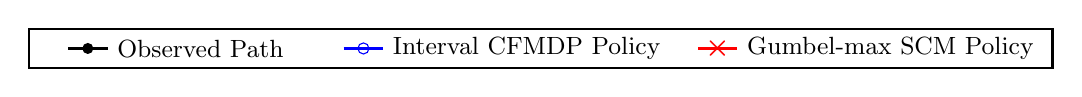
\begin{tikzpicture}[scale=1.0, every node/.style={scale=1.0}]
            \draw[thick, black] (-3, -0.25) rectangle (10, 0.25);
            %
            \draw[black, line width=1pt] (-2.5, 0.0) -- (-2,0.0);
            \fill[black] (-2.25,0.0) circle (2pt); %
            \node[right] at (-2,0.0) {\small Observed Path};
            
            %
            \draw[blue, line width=1pt] (1.0,0.0) -- (1.5,0.0);
            \node[draw=blue, circle, minimum size=4pt, inner sep=0pt] at (1.25,0.0) {}; %
            \node[right] at (1.5,0.0) {\small Interval CFMDP Policy};
            
            %
            \draw[red, line width=1pt] (5.5,0) -- (6,0);
            \node[red] at (5.75,0) {$\boldsymbol{\times}$}; %
            \node[right] at (6,0) {\small Gumbel-max SCM Policy};
        \end{tikzpicture}
    }\\
    %
    \subfigure[\footnotesize Lowest cumulative reward: Interval CFMDP ($312$), Gumbel-max SCM ($312$)]{%
        \resizebox{0.76\columnwidth}{!}{
             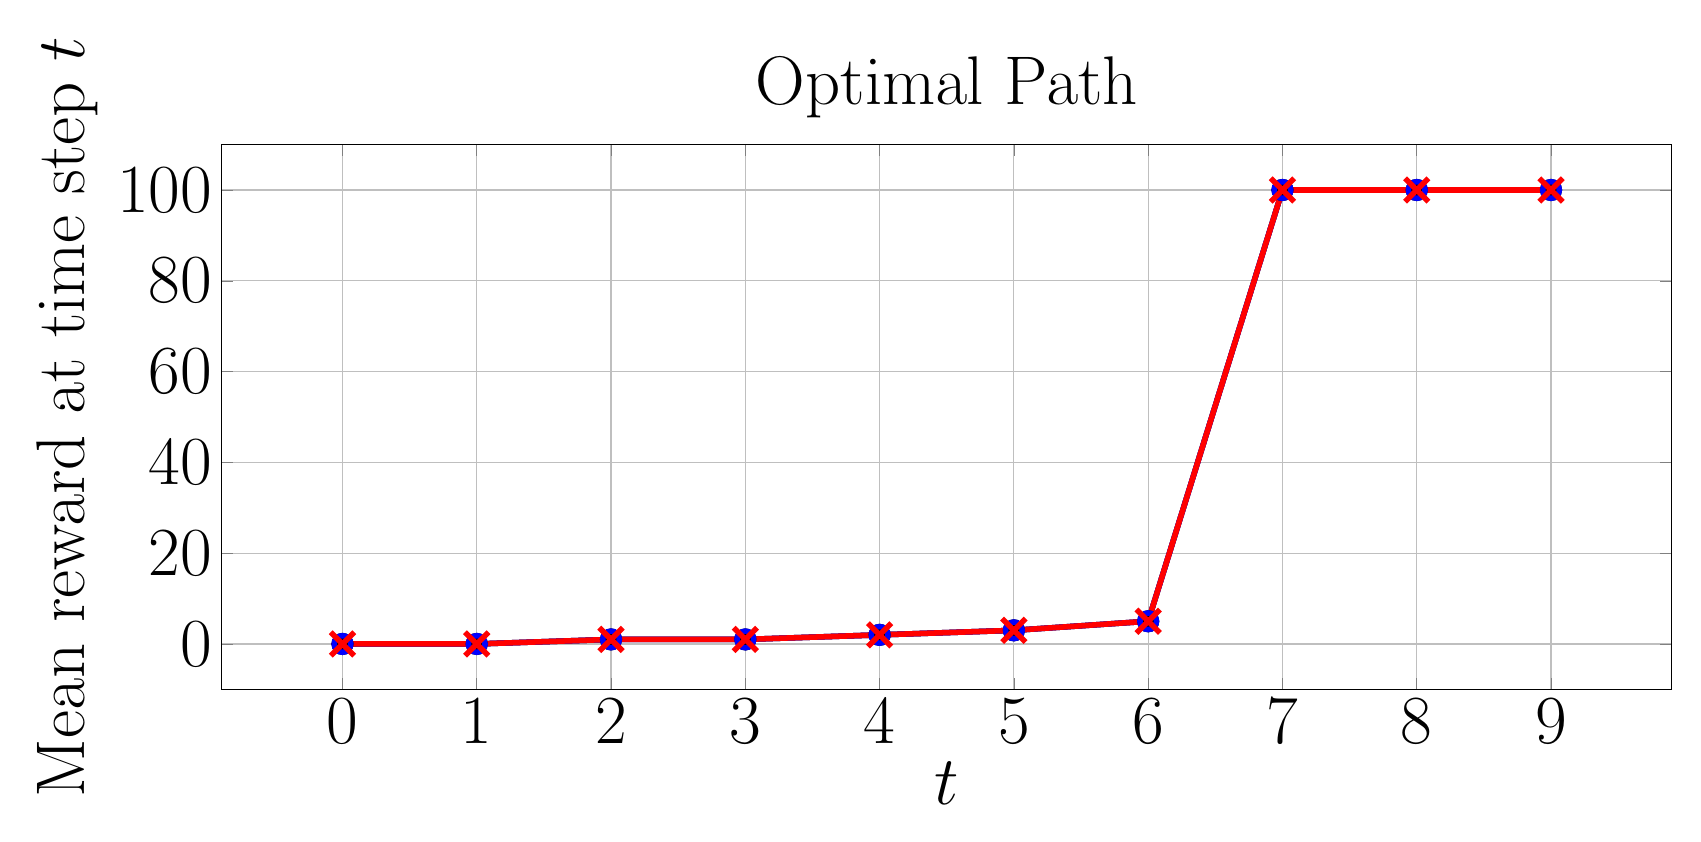
\begin{tikzpicture}
                \begin{axis}[
                    xlabel={$t$},
                    ylabel={Mean reward at time step $t$},
                    title={Optimal Path},
                    grid=both,
                    width=20cm, height=8.5cm,
                    every axis/.style={font=\Huge},
                    %
                ]
                \addplot[
                    color=black, %
                    mark=*, %
                    line width=2pt,
                    mark size=3pt,
                    error bars/.cd,
                    y dir=both, %
                    y explicit, %
                    error bar style={line width=1pt,solid},
                    error mark options={line width=1pt,mark size=4pt,rotate=90}
                ]
                coordinates {
                    (0, 0.0)  +- (0, 0.0)
                    (1, 0.0)  +- (0, 0.0) 
                    (2, 1.0)  +- (0, 0.0) 
                    (3, 1.0)  +- (0, 0.0)
                    (4, 2.0)  +- (0, 0.0)
                    (5, 3.0) +- (0, 0.0)
                    (6, 5.0) +- (0, 0.0)
                    (7, 100.0) +- (0, 0.0)
                    (8, 100.0) +- (0, 0.0)
                    (9, 100.0) +- (0, 0.0)
                };
                %
                \addplot[
                    color=blue, %
                    mark=o, %
                    line width=2pt,
                    mark size=3pt,
                    error bars/.cd,
                    y dir=both, %
                    y explicit, %
                    error bar style={line width=1pt,solid},
                    error mark options={line width=1pt,mark size=4pt,rotate=90}
                ]
                 coordinates {
                    (0, 0.0)  +- (0, 0.0)
                    (1, 0.0)  +- (0, 0.0) 
                    (2, 1.0)  +- (0, 0.0) 
                    (3, 1.0)  +- (0, 0.0)
                    (4, 2.0)  +- (0, 0.0)
                    (5, 3.0) +- (0, 0.0)
                    (6, 5.0) +- (0, 0.0)
                    (7, 100.0) +- (0, 0.0)
                    (8, 100.0) +- (0, 0.0)
                    (9, 100.0) +- (0, 0.0)
                };
                %
                \addplot[
                    color=red, %
                    mark=x, %
                    line width=2pt,
                    mark size=6pt,
                    error bars/.cd,
                    y dir=both, %
                    y explicit, %
                    error bar style={line width=1pt,solid},
                    error mark options={line width=1pt,mark size=4pt,rotate=90}
                ]
                coordinates {
                    (0, 0.0)  +- (0, 0.0)
                    (1, 0.0)  +- (0, 0.0) 
                    (2, 1.0)  +- (0, 0.0) 
                    (3, 1.0)  +- (0, 0.0)
                    (4, 2.0)  +- (0, 0.0)
                    (5, 3.0) +- (0, 0.0)
                    (6, 5.0) +- (0, 0.0)
                    (7, 100.0) +- (0, 0.0)
                    (8, 100.0) +- (0, 0.0)
                    (9, 100.0) +- (0, 0.0)
                };
                \end{axis}
            \end{tikzpicture}
         }
    }
    \hspace{1cm}
    \subfigure[\footnotesize Lowest cumulative reward: Interval CFMDP ($19$), Gumbel-max SCM ($-88$)]{%
         \resizebox{0.76\columnwidth}{!}{
            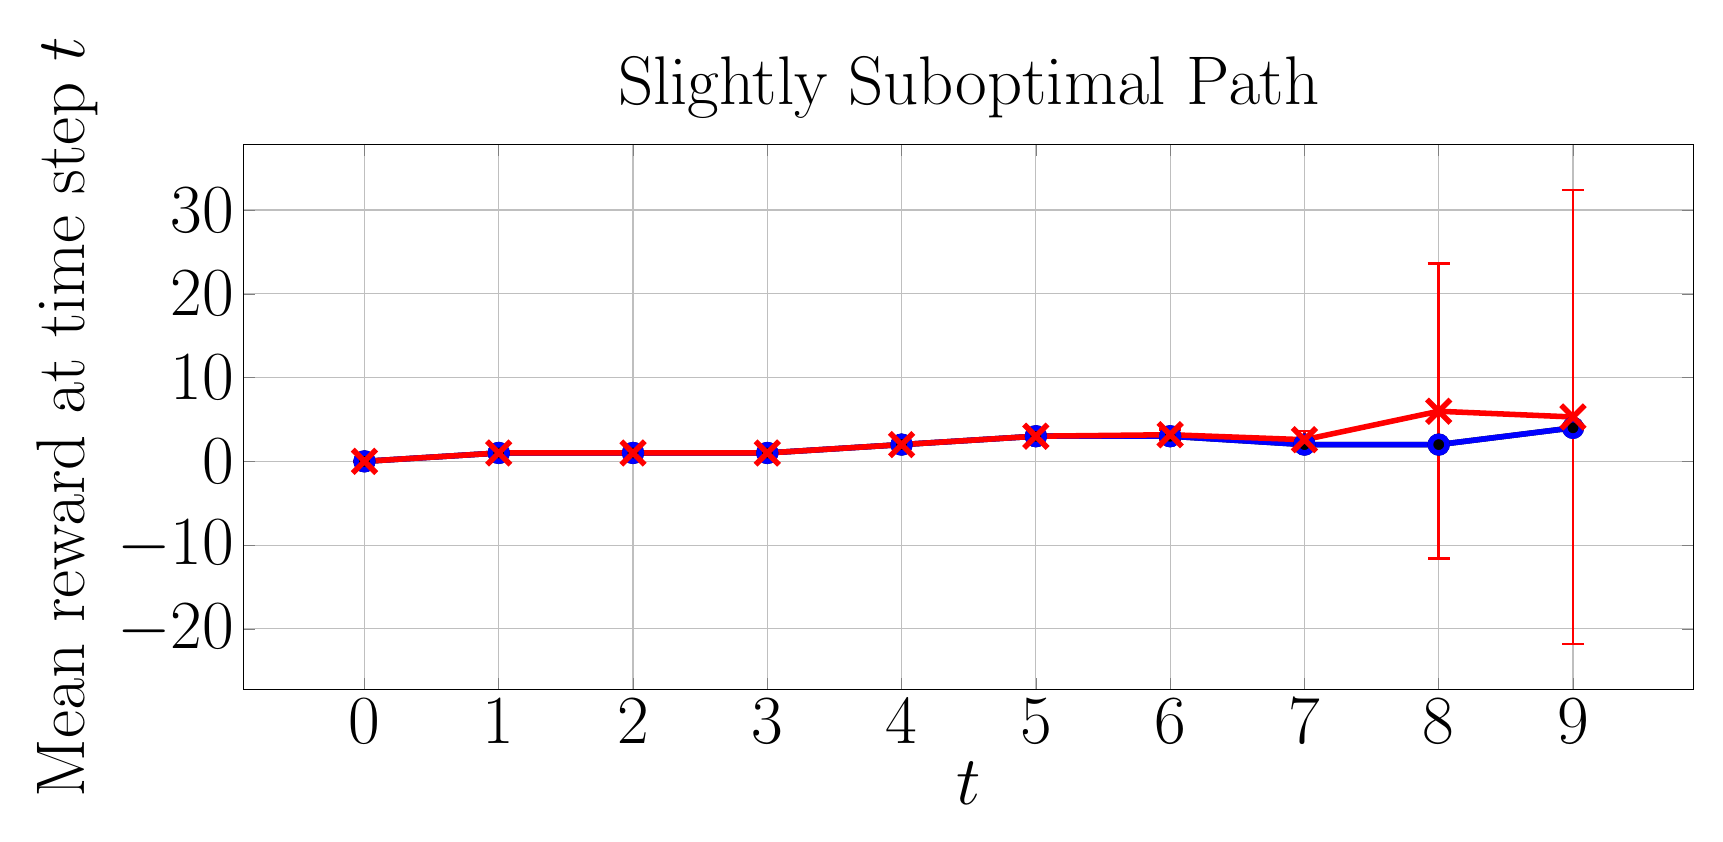
\begin{tikzpicture}
                \begin{axis}[
                    xlabel={$t$},
                    ylabel={Mean reward at time step $t$},
                    title={Slightly Suboptimal Path},
                    grid=both,
                    width=20cm, height=8.5cm,
                    every axis/.style={font=\Huge},
                    %
                ]
                \addplot[
                    color=black, %
                    mark=*, %
                    line width=2pt,
                    mark size=3pt,
                    error bars/.cd,
                    y dir=both, %
                    y explicit, %
                    error bar style={line width=1pt,solid},
                    error mark options={line width=1pt,mark size=4pt,rotate=90}
                ]
              coordinates {
                    (0, 0.0)  +- (0, 0.0)
                    (1, 1.0)  +- (0, 0.0) 
                    (2, 1.0)  +- (0, 0.0) 
                    (3, 1.0)  +- (0, 0.0)
                    (4, 2.0)  +- (0, 0.0)
                    (5, 3.0) +- (0, 0.0)
                    (6, 3.0) +- (0, 0.0)
                    (7, 2.0) +- (0, 0.0)
                    (8, 2.0) +- (0, 0.0)
                    (9, 4.0) +- (0, 0.0)
                };
                %
                \addplot[
                    color=blue, %
                    mark=o, %
                    line width=2pt,
                    mark size=3pt,
                    error bars/.cd,
                    y dir=both, %
                    y explicit, %
                    error bar style={line width=1pt,solid},
                    error mark options={line width=1pt,mark size=4pt,rotate=90}
                ]
              coordinates {
                    (0, 0.0)  +- (0, 0.0)
                    (1, 1.0)  +- (0, 0.0) 
                    (2, 1.0)  +- (0, 0.0) 
                    (3, 1.0)  +- (0, 0.0)
                    (4, 2.0)  +- (0, 0.0)
                    (5, 3.0) +- (0, 0.0)
                    (6, 3.0) +- (0, 0.0)
                    (7, 2.0) +- (0, 0.0)
                    (8, 2.0) +- (0, 0.0)
                    (9, 4.0) +- (0, 0.0)
                };
                %
                \addplot[
                    color=red, %
                    mark=x, %
                    line width=2pt,
                    mark size=6pt,
                    error bars/.cd,
                    y dir=both, %
                    y explicit, %
                    error bar style={line width=1pt,solid},
                    error mark options={line width=1pt,mark size=4pt,rotate=90}
                ]
                coordinates {
                    (0, 0.0)  +- (0, 0.0)
                    (1, 1.0)  +- (0, 0.0) 
                    (2, 1.0)  +- (0, 0.0) 
                    (3, 1.0)  +- (0, 0.0)
                    (4, 2.0)  += (0, 0.0)
                    (5, 3.0)  += (0, 0.0)
                    (6, 3.17847) += (0, 0.62606746) -= (0, 0.62606746)
                    (7, 2.5832885) += (0, 1.04598233) -= (0, 1.04598233)
                    (8, 5.978909) += (0, 17.60137623) -= (0, 17.60137623)
                    (9, 5.297059) += (0, 27.09227512) -= (0, 27.09227512)
                };
                \end{axis}
            \end{tikzpicture}
         }
    }\\[-1.5pt]
    \subfigure[\footnotesize Lowest cumulative reward: Interval CFMDP ($14$), Gumbel-max SCM ($-598$)]{%
         \resizebox{0.76\columnwidth}{!}{
             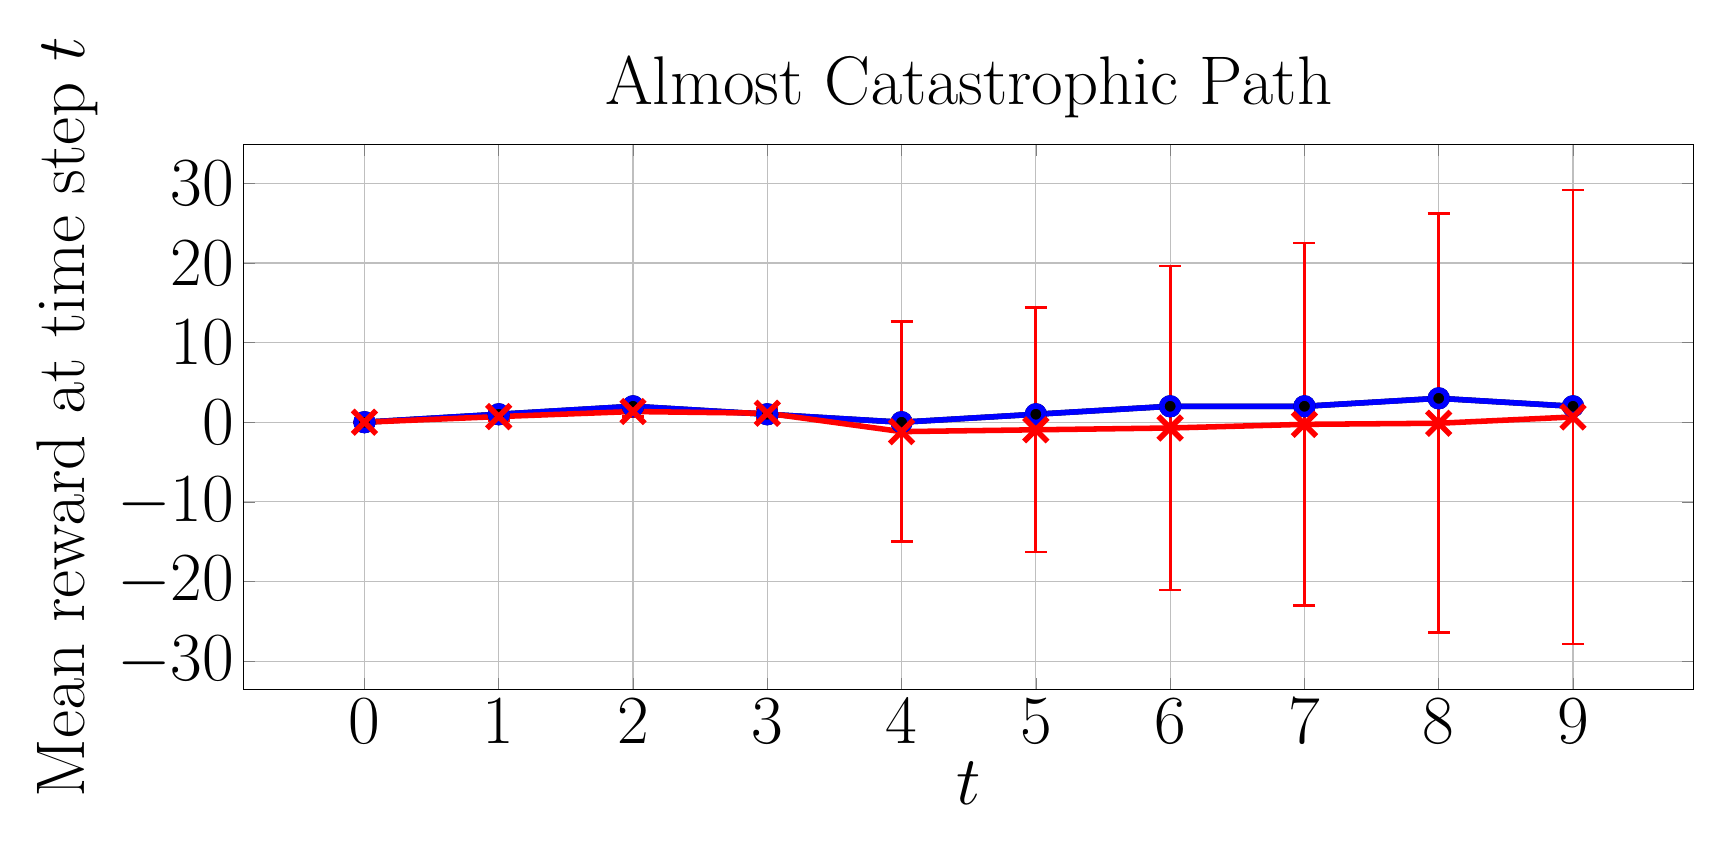
\begin{tikzpicture}
                \begin{axis}[
                    xlabel={$t$},
                    ylabel={Mean reward at time step $t$},
                    title={Almost Catastrophic Path},
                    grid=both,
                    width=20cm, height=8.5cm,
                    every axis/.style={font=\Huge},
                    %
                ]
                \addplot[
                    color=black, %
                    mark=*, %
                    line width=2pt,
                    mark size=3pt,
                    error bars/.cd,
                    y dir=both, %
                    y explicit, %
                    error bar style={line width=1pt,solid},
                    error mark options={line width=1pt,mark size=4pt,rotate=90}
                ]
                coordinates {
                    (0, 0.0)  +- (0, 0.0)
                    (1, 1.0)  +- (0, 0.0) 
                    (2, 2.0)  +- (0, 0.0) 
                    (3, 1.0)  +- (0, 0.0)
                    (4, 0.0)  +- (0, 0.0)
                    (5, 1.0) +- (0, 0.0)
                    (6, 2.0) +- (0, 0.0)
                    (7, 2.0) +- (0, 0.0)
                    (8, 3.0) +- (0, 0.0)
                    (9, 2.0) +- (0, 0.0)
                };
                %
                \addplot[
                    color=blue, %
                    mark=o, %
                    line width=2pt,
                    mark size=3pt,
                    error bars/.cd,
                    y dir=both, %
                    y explicit, %
                    error bar style={line width=1pt,solid},
                    error mark options={line width=1pt,mark size=4pt,rotate=90}
                ]
                coordinates {
                    (0, 0.0)  +- (0, 0.0)
                    (1, 1.0)  +- (0, 0.0) 
                    (2, 2.0)  +- (0, 0.0) 
                    (3, 1.0)  +- (0, 0.0)
                    (4, 0.0)  +- (0, 0.0)
                    (5, 1.0) +- (0, 0.0)
                    (6, 2.0) +- (0, 0.0)
                    (7, 2.0) +- (0, 0.0)
                    (8, 3.0) +- (0, 0.0)
                    (9, 2.0) +- (0, 0.0)
                };
                %
                \addplot[
                    color=red, %
                    mark=x, %
                    line width=2pt,
                    mark size=6pt,
                    error bars/.cd,
                    y dir=both, %
                    y explicit, %
                    error bar style={line width=1pt,solid},
                    error mark options={line width=1pt,mark size=4pt,rotate=90}
                ]
                coordinates {
                    (0, 0.0)  +- (0, 0.0)
                    (1, 0.7065655)  +- (0, 0.4553358) 
                    (2, 1.341673)  +- (0, 0.67091621) 
                    (3, 1.122926)  +- (0, 0.61281824)
                    (4, -1.1821935)  +- (0, 13.82444042)
                    (5, -0.952399)  +- (0, 15.35195457)
                    (6, -0.72672) +- (0, 20.33508414)
                    (7, -0.268983) +- (0, 22.77861454)
                    (8, -0.1310835) +- (0, 26.31013314)
                    (9, 0.65806) +- (0, 28.50670214)
                };
                %
            %
            %
            %
            %
            %
            %
            %
            %
            %
            %
            %
            %
            %
            %
            %
            %
            %
            %
                \end{axis}
            \end{tikzpicture}
         }
    }
    \hspace{1cm}
    \subfigure[\footnotesize Lowest cumulative reward: Interval CFMDP ($-698$), Gumbel-max SCM ($-698$)]{%
         \resizebox{0.76\columnwidth}{!}{
            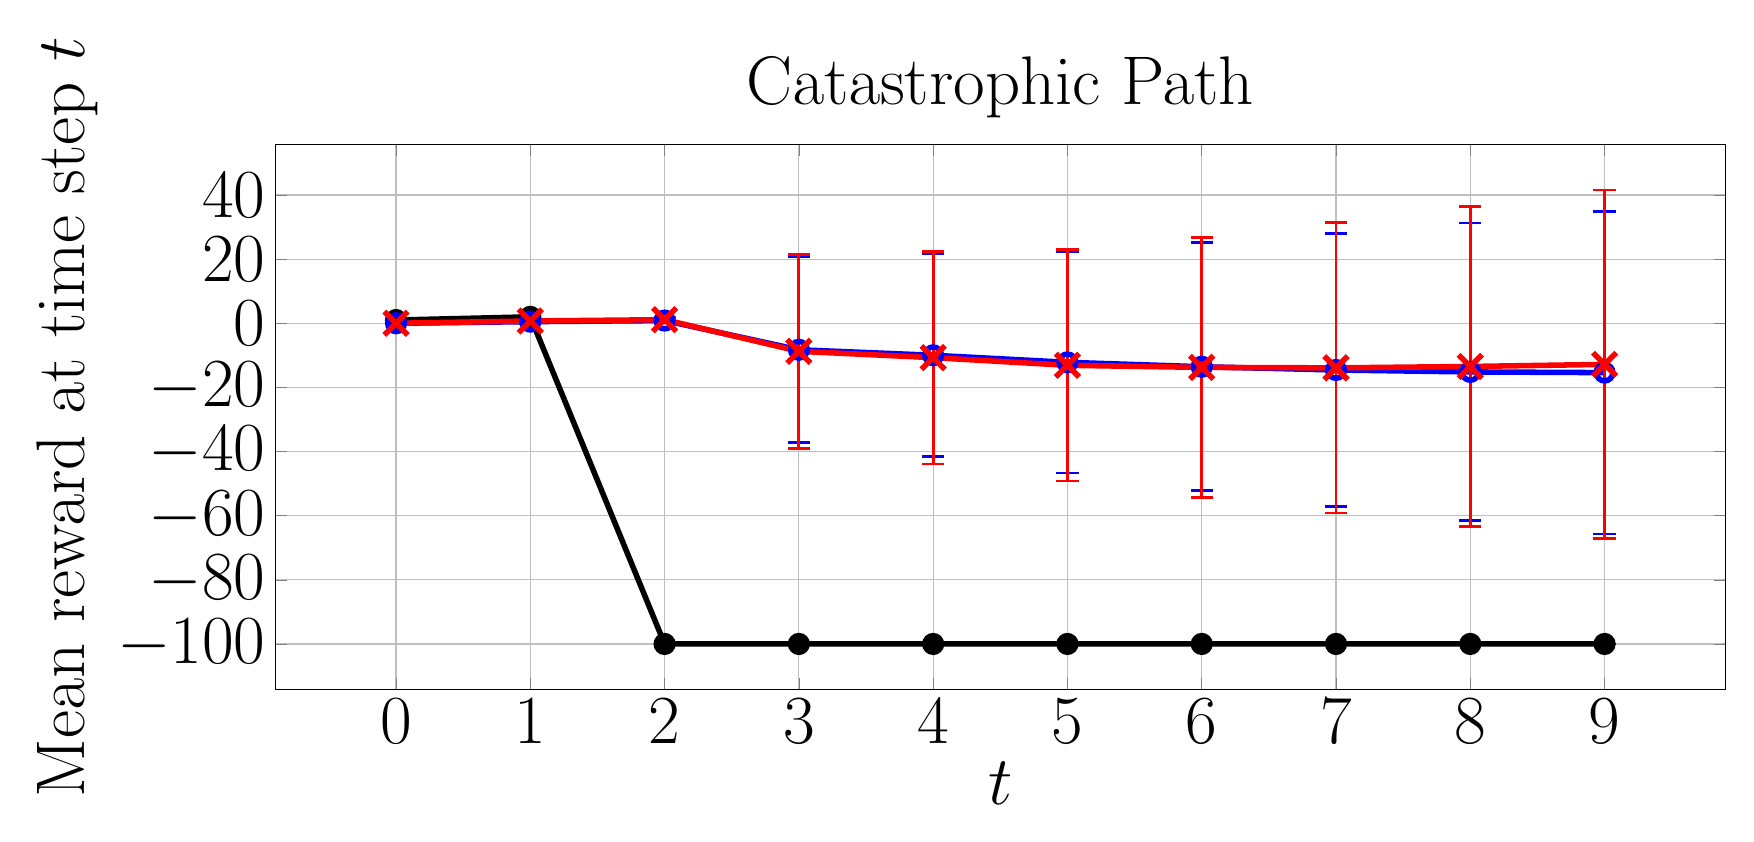
\begin{tikzpicture}
                \begin{axis}[
                    xlabel={$t$},
                    ylabel={Mean reward at time step $t$},
                    title={Catastrophic Path},
                    grid=both,
                    width=20cm, height=8.5cm,
                    every axis/.style={font=\Huge},
                    %
                ]
                \addplot[
                    color=black, %
                    mark=*, %
                    line width=2pt,
                    mark size=3pt,
                    error bars/.cd,
                    y dir=both, %
                    y explicit, %
                    error bar style={line width=1pt,solid},
                    error mark options={line width=1pt,mark size=4pt,rotate=90}
                ]
                coordinates {
                    (0, 1.0)  +- (0, 0.0)
                    (1, 2.0)  +- (0, 0.0) 
                    (2, -100.0)  +- (0, 0.0) 
                    (3, -100.0)  +- (0, 0.0)
                    (4, -100.0)  +- (0, 0.0)
                    (5, -100.0) +- (0, 0.0)
                    (6, -100.0) +- (0, 0.0)
                    (7, -100.0) +- (0, 0.0)
                    (8, -100.0) +- (0, 0.0)
                    (9, -100.0) +- (0, 0.0)
                };
                %
                \addplot[
                    color=blue, %
                    mark=o, %
                    line width=2pt,
                    mark size=3pt,
                    error bars/.cd,
                    y dir=both, %
                    y explicit, %
                    error bar style={line width=1pt,solid},
                    error mark options={line width=1pt,mark size=4pt,rotate=90}
                ]
                coordinates {
                    (0, 0.0)  +- (0, 0.0)
                    (1, 0.504814)  +- (0, 0.49997682) 
                    (2, 0.8439835)  +- (0, 0.76831917) 
                    (3, -8.2709165)  +- (0, 28.93656754)
                    (4, -9.981082)  +- (0, 31.66825363)
                    (5, -12.1776325) +- (0, 34.53463233)
                    (6, -13.556076) +- (0, 38.62845372)
                    (7, -14.574418) +- (0, 42.49603359)
                    (8, -15.1757075) +- (0, 46.41913968)
                    (9, -15.3900395) +- (0, 50.33563368)
                };
                %
                \addplot[
                    color=red, %
                    mark=x, %
                    line width=2pt,
                    mark size=6pt,
                    error bars/.cd,
                    y dir=both, %
                    y explicit, %
                    error bar style={line width=1pt,solid},
                    error mark options={line width=1pt,mark size=4pt,rotate=90}
                ]
                coordinates {
                    (0, 0.0)  +- (0, 0.0)
                    (1, 0.701873)  +- (0, 0.45743556) 
                    (2, 1.1227805)  +- (0, 0.73433129) 
                    (3, -8.7503255)  +- (0, 30.30257976)
                    (4, -10.722092)  +- (0, 33.17618589)
                    (5, -13.10721)  +- (0, 36.0648089)
                    (6, -13.7631645) +- (0, 40.56553451)
                    (7, -13.909043) +- (0, 45.23829402)
                    (8, -13.472517) +- (0, 49.96270296)
                    (9, -12.8278835) +- (0, 54.38618735)
                };
                %
            %
            %
            %
            %
            %
            %
            %
            %
            %
            %
            %
            %
            %
            %
            %
            %
            %
            %
                \end{axis}
            \end{tikzpicture}
         }
    }
    \caption{Average instant reward of CF paths induced by policies on GridWorld $p=0.4$.}
    \label{fig: reward p=0.4}
\end{figure*}

\subsection{Experimental Setup}
To compare policy performance, we measure the average rewards of counterfactual paths induced by our policy and the Gumbel-max policy by uniformly sampling $200$ counterfactual MDPs from the ICFMDP and generating $10,000$ counterfactual paths over each sampled CFMDP. \jl{Since the interval CFMDP depends on the observed path, we select $4$  paths of varying optimality to evaluate how the observed path impacts the performance of both policies: an optimal path, a slightly suboptimal path that could reach the optimal reward with a few changes, a catastrophic path that enters a catastrophic, terminal state with low reward, and an almost catastrophic path that was close to entering a catastrophic state.} When measuring the average probability bound widths and execution time needed to generate the ICFMDPs, we averaged over $20$ randomly generated observed paths
\footnote{Further training details are provided in Appendix \ref{app: training details}, and the code is provided at \href{https://github.com/ddv-lab/robust-cf-inference-in-MDPs}{https://github.com/ddv-lab/robust-cf-inference-in-MDPs}
%
%
.}.

\subsection{GridWorld}
\jl{The GridWorld MDP is a $4 \times 4$ grid where an agent must navigate from the top-left corner to the goal state in the bottom-right corner, avoiding a dangerous terminal state in the centre. At each time step, the agent can move up, down, left, or right, but there is a small probability (controlled by hyper-parameter $p$) of moving in an unintended direction. As the agent nears the goal, the reward for each state increases, culminating in a reward of $+100$ for reaching the goal. Entering the dangerous state results in a penalty of $-100$. We use two versions of GridWorld: a less stochastic version with $p=0.9$ (i.e., $90$\% chance of moving in the chosen direction) and a more stochastic version with $p=0.4$.}

\paragraph{GridWorld ($p=0.9$)}
When $p=0.9$, the counterfactual probability bounds are typically narrow (see Table \ref{tab:nonzero_probs} for average measurements). Consequently, as shown in Figure \ref{fig: reward p=0.9}, both policies are nearly identical and perform similarly well across the optimal, slightly suboptimal, and catastrophic paths.
%
However, for the almost catastrophic path, the interval CFMDP path is more conservative and follows the observed path more closely (as this is where the probability bounds are narrowest), which typically requires one additional step to reach the goal state than the Gumbel-max SCM policy.
%

\paragraph{GridWorld ($p=0.4$)}
\jl{When $p=0.4$, the GridWorld environment becomes more uncertain, increasing the risk of entering the dangerous state even if correct actions are chosen. Thus, as shown in Figure \ref{fig: reward p=0.4}, the interval CFMDP policy adopts a more conservative approach, avoiding deviation from the observed policy if it cannot guarantee higher counterfactual rewards (see the slightly suboptimal and almost catastrophic paths), whereas the Gumbel-max SCM is inconsistent: it can yield higher rewards, but also much lower rewards, reflected in the wide error bars.} For the catastrophic path, both policies must deviate from the observed path to achieve a higher reward and, in this case, perform similarly.
%
%
%
%
\subsection{Sepsis}
The Sepsis MDP \citep{oberst2019counterfactual} simulates trajectories of Sepsis patients. Each state consists of four vital signs (heart rate, blood pressure, oxygen concentration, and glucose levels), categorised as low, normal, or high.
and three treatments that can be toggled on/off at each time step (8 actions in total). Unlike \citet{oberst2019counterfactual}, we scale rewards based on the number of out-of-range vital signs, between $-1000$ (patient dies) and $1000$ (patient discharged). \jl{Like the GridWorld $p=0.4$ experiment, the Sepsis MDP is highly uncertain, as many states are equally likely to lead to optimal and poor outcomes. Thus, as shown in Figure \ref{fig: reward sepsis}, both policies follow the observed optimal and almost catastrophic paths to guarantee rewards are no worse than the observation.} However, improving the catastrophic path requires deviating from the observation. Here, the Gumbel-max SCM policy, on average, performs better than the interval CFMDP policy. But, since both policies have lower bounds clipped at $-1000$, neither policy reliably improves over the observation. In contrast, for the slightly suboptimal path, the interval CFMDP policy performs significantly better, shown by its higher lower bounds. 
Moreover, in these two cases, the worst-case counterfactual path generated by the interval CFMDP policy is better than that of the Gumbel-max SCM policy,
indicating its greater robustness.
%
\begin{figure*}
    \centering
     \resizebox{0.6\textwidth}{!}{
        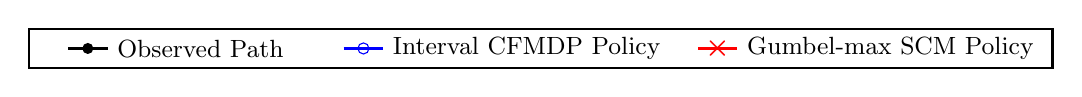
\begin{tikzpicture}[scale=1.0, every node/.style={scale=1.0}]
            \draw[thick, black] (-3, -0.25) rectangle (10, 0.25);
            %
            \draw[black, line width=1pt] (-2.5, 0.0) -- (-2,0.0);
            \fill[black] (-2.25,0.0) circle (2pt); %
            \node[right] at (-2,0.0) {\small Observed Path};
            
            %
            \draw[blue, line width=1pt] (1.0,0.0) -- (1.5,0.0);
            \node[draw=blue, circle, minimum size=4pt, inner sep=0pt] at (1.25,0.0) {}; %
            \node[right] at (1.5,0.0) {\small Interval CFMDP Policy};
            
            %
            \draw[red, line width=1pt] (5.5,0) -- (6,0);
            \node[red] at (5.75,0) {$\boldsymbol{\times}$}; %
            \node[right] at (6,0) {\small Gumbel-max SCM Policy};
        \end{tikzpicture}
    }\\
    \subfigure[\footnotesize Lowest cumulative reward: Interval CFMDP ($8000$), Gumbel-max SCM ($8000$)]{%
         \resizebox{0.76\columnwidth}{!}{
             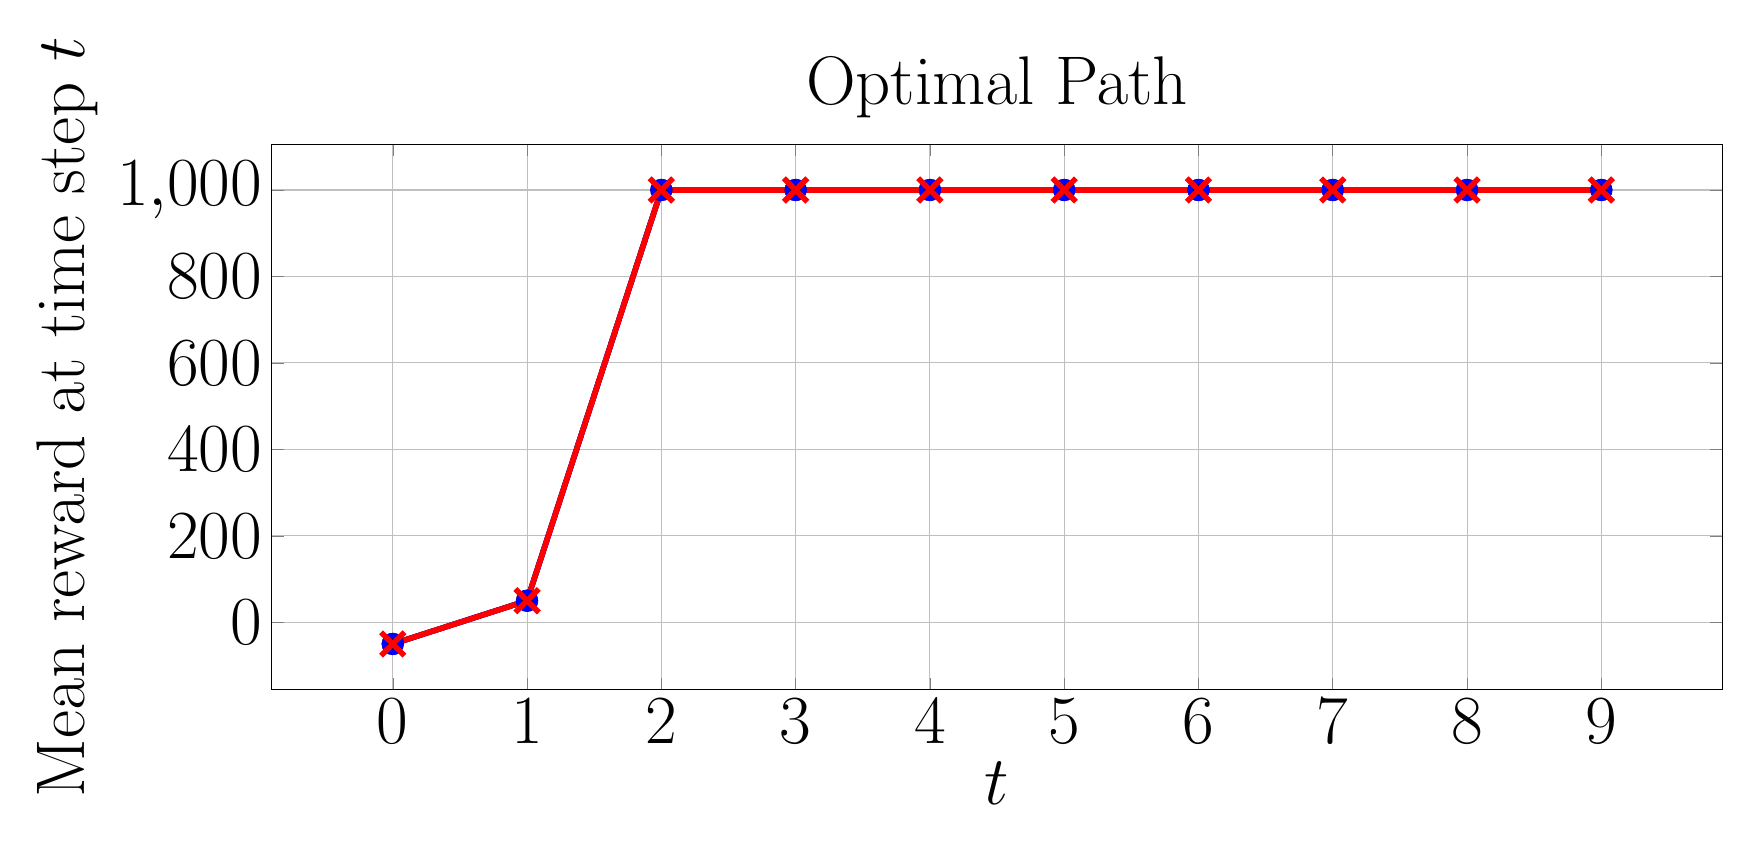
\begin{tikzpicture}
                \begin{axis}[
                    xlabel={$t$},
                    ylabel={Mean reward at time step $t$},
                    title={Optimal Path},
                    grid=both,
                    width=20cm, height=8.5cm,
                    every axis/.style={font=\Huge},
                    %
                ]
                \addplot[
                    color=black, %
                    mark=*, %
                    line width=2pt,
                    mark size=3pt,
                ]
                coordinates {
                    (0, -50.0)
                    (1, 50.0)
                    (2, 1000.0)
                    (3, 1000.0)
                    (4, 1000.0)
                    (5, 1000.0)
                    (6, 1000.0)
                    (7, 1000.0)
                    (8, 1000.0)
                    (9, 1000.0)
                };
                %
                \addplot[
                    color=blue, %
                    mark=o, %
                    line width=2pt,
                    mark size=3pt,
                    error bars/.cd,
                    y dir=both, %
                    y explicit, %
                    error bar style={line width=1pt,solid},
                    error mark options={line width=1pt,mark size=4pt,rotate=90}
                ]
                coordinates {
                    (0, -50.0)  +- (0, 0.0)
                    (1, 50.0)  +- (0, 0.0) 
                    (2, 1000.0)  +- (0, 0.0) 
                    (3, 1000.0)  +- (0, 0.0)
                    (4, 1000.0)  +- (0, 0.0)
                    (5, 1000.0) +- (0, 0.0)
                    (6, 1000.0) +- (0, 0.0)
                    (7, 1000.0) +- (0, 0.0)
                    (8, 1000.0) +- (0, 0.0)
                    (9, 1000.0) +- (0, 0.0)
                };
                %
                \addplot[
                    color=red, %
                    mark=x, %
                    line width=2pt,
                    mark size=6pt,
                    error bars/.cd,
                    y dir=both, %
                    y explicit, %
                    error bar style={line width=1pt,solid},
                    error mark options={line width=1pt,mark size=4pt,rotate=90}
                ]
                coordinates {
                    (0, -50.0)  +- (0, 0.0)
                    (1, 50.0)  +- (0, 0.0) 
                    (2, 1000.0)  +- (0, 0.0) 
                    (3, 1000.0)  +- (0, 0.0)
                    (4, 1000.0)  +- (0, 0.0)
                    (5, 1000.0) +- (0, 0.0)
                    (6, 1000.0) +- (0, 0.0)
                    (7, 1000.0) +- (0, 0.0)
                    (8, 1000.0) +- (0, 0.0)
                    (9, 1000.0) +- (0, 0.0)
                };
                %
                \end{axis}
            \end{tikzpicture}
         }
    }
    \hspace{1cm}
    \subfigure[\footnotesize Lowest cumulative reward: Interval CFMDP ($-5980$), Gumbel-max SCM ($-8000$)]{%
         \resizebox{0.76\columnwidth}{!}{
            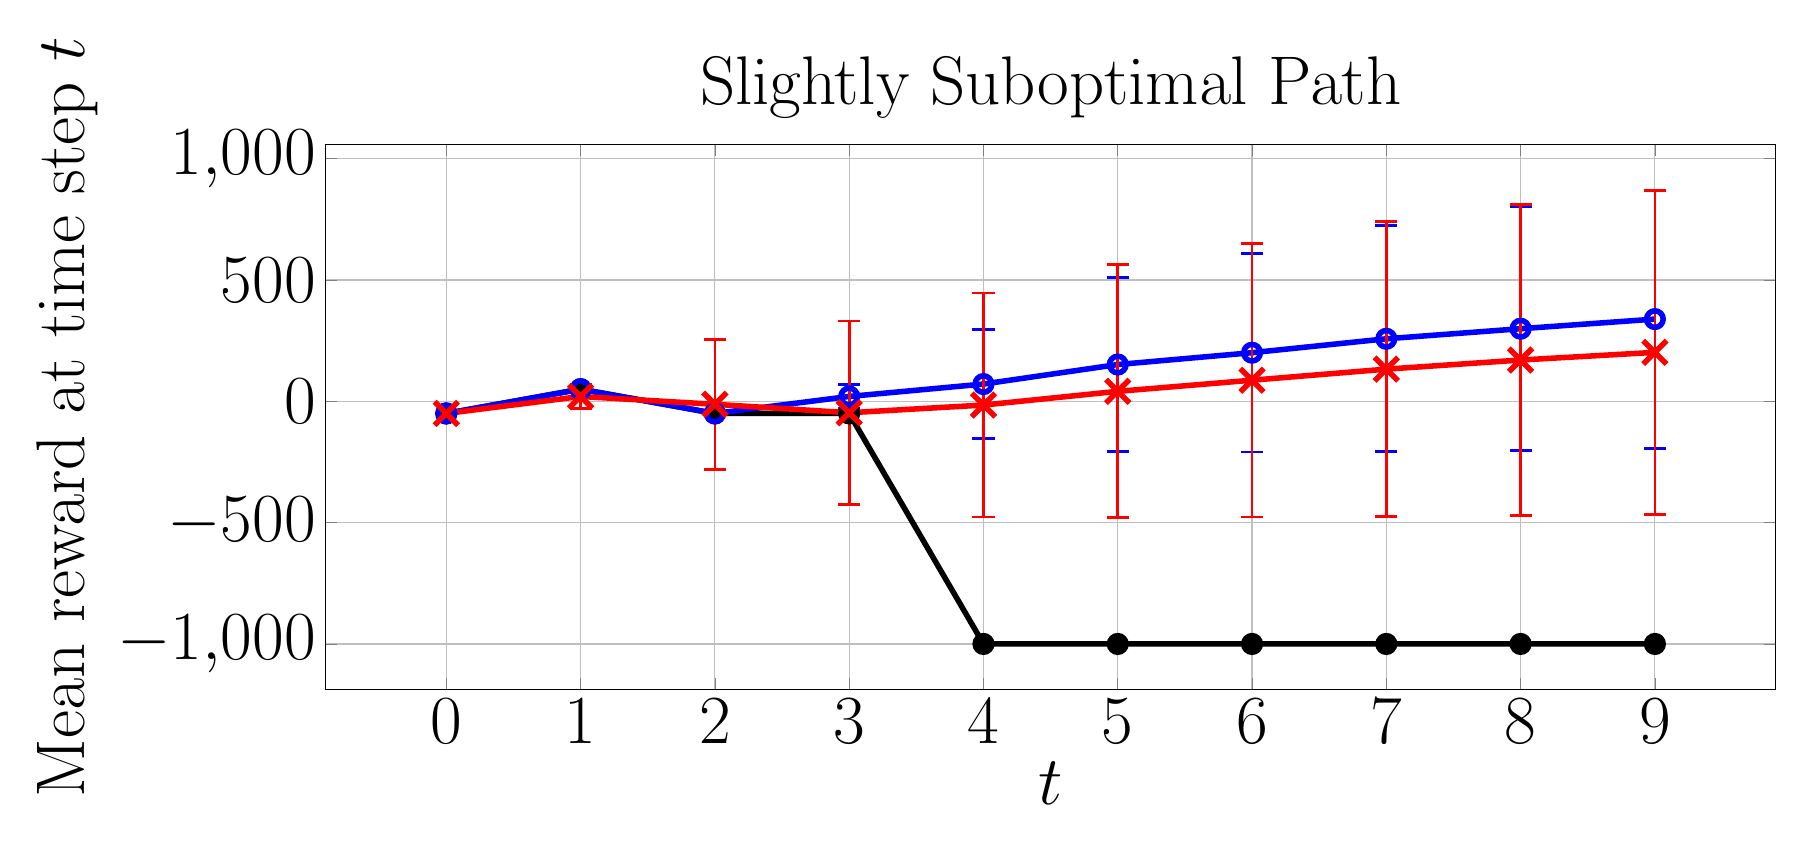
\begin{tikzpicture}
                \begin{axis}[
                    xlabel={$t$},
                    ylabel={Mean reward at time step $t$},
                    title={Slightly Suboptimal Path},
                    grid=both,
                    width=20cm, height=8.5cm,
                    every axis/.style={font=\Huge},
                    %
                ]
               \addplot[
                    color=black, %
                    mark=*, %
                    line width=2pt,
                    mark size=3pt,
                ]
                coordinates {
                    (0, -50.0)
                    (1, 50.0)
                    (2, -50.0)
                    (3, -50.0)
                    (4, -1000.0)
                    (5, -1000.0)
                    (6, -1000.0)
                    (7, -1000.0)
                    (8, -1000.0)
                    (9, -1000.0)
                };
                %
                \addplot[
                    color=blue, %
                    mark=o, %
                    line width=2pt,
                    mark size=3pt,
                    error bars/.cd,
                    y dir=both, %
                    y explicit, %
                    error bar style={line width=1pt,solid},
                    error mark options={line width=1pt,mark size=4pt,rotate=90}
                ]
                coordinates {
                    (0, -50.0)  +- (0, 0.0)
                    (1, 50.0)  +- (0, 0.0) 
                    (2, -50.0)  +- (0, 0.0) 
                    (3, 20.0631)  +- (0, 49.97539413)
                    (4, 71.206585)  +- (0, 226.02033693)
                    (5, 151.60797) +- (0, 359.23292559)
                    (6, 200.40593) +- (0, 408.86185176)
                    (7, 257.77948) +- (0, 466.10372804)
                    (8, 299.237465) +- (0, 501.82579506)
                    (9, 338.9129) +- (0, 532.06124996)
                };
                %
                \addplot[
                    color=red, %
                    mark=x, %
                    line width=2pt,
                    mark size=6pt,
                    error bars/.cd,
                    y dir=both, %
                    y explicit, %
                    error bar style={line width=1pt,solid},
                    error mark options={line width=1pt,mark size=4pt,rotate=90}
                ]
                coordinates {
                    (0, -50.0)  +- (0, 0.0)
                    (1, 20.00736)  +- (0, 49.99786741) 
                    (2, -12.282865)  +- (0, 267.598755) 
                    (3, -47.125995)  +- (0, 378.41755832)
                    (4, -15.381965)  +- (0, 461.77616558)
                    (5, 41.15459) +- (0, 521.53189262)
                    (6, 87.01595) +- (0, 564.22243126 )
                    (7, 132.62376) +- (0, 607.31338037)
                    (8, 170.168145) +- (0, 641.48013693)
                    (9, 201.813135) +- (0, 667.29441777)
                };
                %
                %
                %
                %
                %
                %
                %
                %
                %
                %
                %
                %
                %
                %
                %
                %
                %
                %
                %
                \end{axis}
            \end{tikzpicture}
         }
    }\\[-1.5pt]
    \subfigure[\footnotesize Lowest cumulative reward: Interval CFMDP ($100$), Gumbel-max SCM ($100$)]{%
         \resizebox{0.76\columnwidth}{!}{
             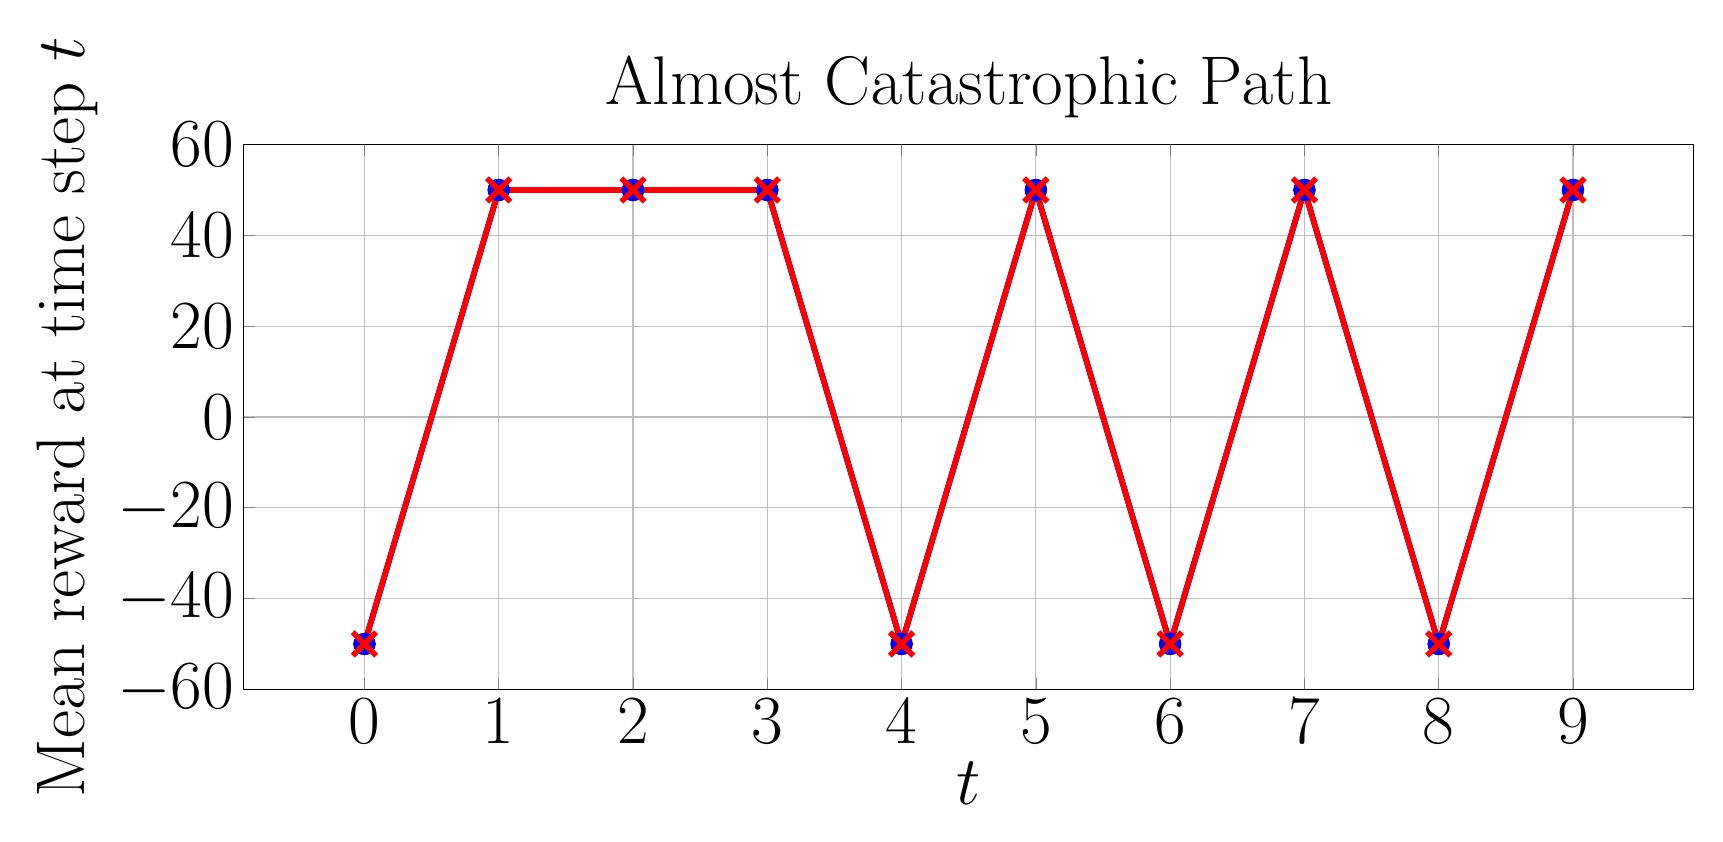
\begin{tikzpicture}
                \begin{axis}[
                    xlabel={$t$},
                    ylabel={Mean reward at time step $t$},
                    title={Almost Catastrophic Path},
                    grid=both,
                    every axis/.style={font=\Huge},
                    width=20cm, height=8.5cm,
                    %
                ]
               \addplot[
                    color=black, %
                    mark=*, %
                    line width=2pt,
                    mark size=3pt,
                ]
                coordinates {
                    (0, -50.0)
                    (1, 50.0)
                    (2, 50.0)
                    (3, 50.0)
                    (4, -50.0)
                    (5, 50.0)
                    (6, -50.0)
                    (7, 50.0)
                    (8, -50.0)
                    (9, 50.0)
                };
                %
                %
                \addplot[
                    color=blue, %
                    mark=o, %
                    line width=2pt,
                    mark size=3pt,
                    error bars/.cd,
                    y dir=both, %
                    y explicit, %
                    error bar style={line width=1pt,solid},
                    error mark options={line width=1pt,mark size=4pt,rotate=90}
                ]
                coordinates {
                    (0, -50.0)  +- (0, 0.0)
                    (1, 50.0)  +- (0, 0.0) 
                    (2, 50.0)  +- (0, 0.0) 
                    (3, 50.0)  +- (0, 0.0)
                    (4, -50.0)  +- (0, 0.0)
                    (5, 50.0) +- (0, 0.0)
                    (6, -50.0) +- (0, 0.0)
                    (7, 50.0) +- (0, 0.0)
                    (8, -50.0) +- (0, 0.0)
                    (9, 50.0) +- (0, 0.0)
                };
                %
                \addplot[
                    color=red, %
                    mark=x, %
                    line width=2pt,
                    mark size=6pt,
                    error bars/.cd,
                    y dir=both, %
                    y explicit, %
                    error bar style={line width=1pt,solid},
                    error mark options={line width=1pt,mark size=4pt,rotate=90}
                ]
                coordinates {
                    (0, -50.0)  +- (0, 0.0)
                    (1, 50.0)  +- (0, 0.0) 
                    (2, 50.0)  +- (0, 0.0) 
                    (3, 50.0)  +- (0, 0.0)
                    (4, -50.0)  +- (0, 0.0)
                    (5, 50.0) +- (0, 0.0)
                    (6, -50.0) +- (0, 0.0)
                    (7, 50.0) +- (0, 0.0)
                    (8, -50.0) +- (0, 0.0)
                    (9, 50.0) +- (0, 0.0)
                };
                %
                %
                %
                %
                %
                %
                %
                %
                %
                %
                %
                %
                %
                %
                %
                %
                %
                %
                %
                \end{axis}
            \end{tikzpicture}
         }
    }
    \hspace{1cm}
    \subfigure[\footnotesize Lowest cumulative reward: Interval CFMDP ($-7150$), Gumbel-max SCM ($-9050$)]{%
         \resizebox{0.76\columnwidth}{!}{
            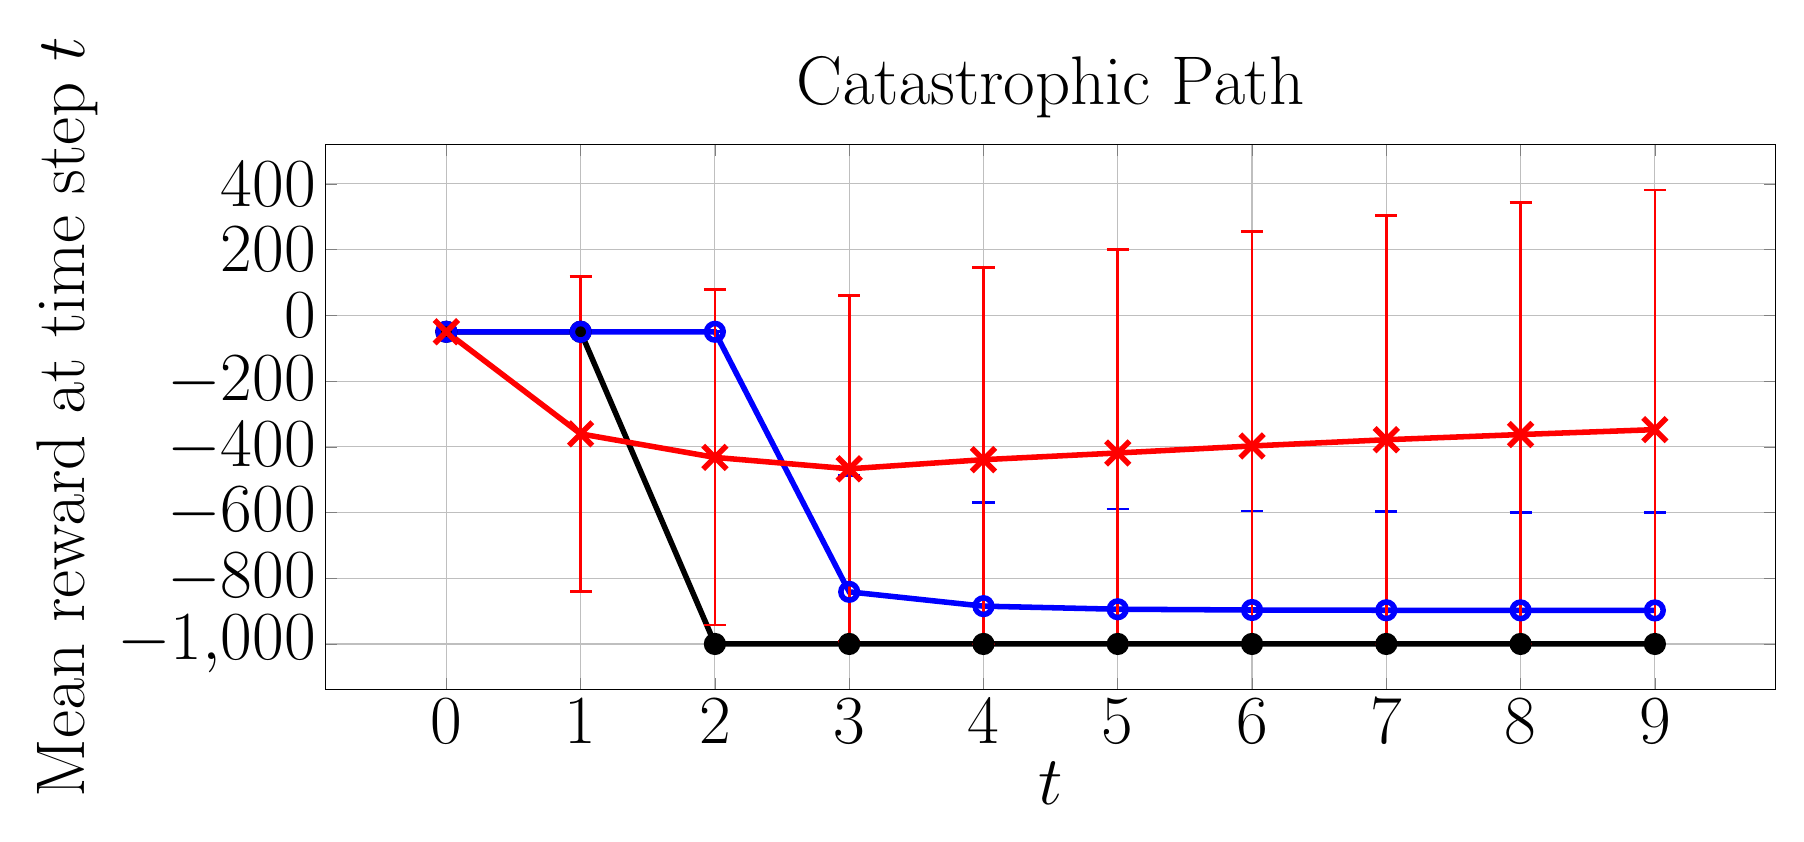
\begin{tikzpicture}
                \begin{axis}[
                    xlabel={$t$},
                    ylabel={Mean reward at time step $t$},
                    title={Catastrophic Path},
                    grid=both,
                    width=20cm, height=8.5cm,
                    every axis/.style={font=\Huge},
                    %
                ]
               \addplot[
                    color=black, %
                    mark=*, %
                    line width=2pt,
                    mark size=3pt,
                ]
                coordinates {
                    (0, -50.0)
                    (1, -50.0)
                    (2, -1000.0)
                    (3, -1000.0)
                    (4, -1000.0)
                    (5, -1000.0)
                    (6, -1000.0)
                    (7, -1000.0)
                    (8, -1000.0)
                    (9, -1000.0)
                };
                %
                %
                \addplot[
                    color=blue, %
                    mark=o, %
                    line width=2pt,
                    mark size=3pt,
                    error bars/.cd,
                    y dir=both, %
                    y explicit, %
                    error bar style={line width=1pt,solid},
                    error mark options={line width=1pt,mark size=4pt,rotate=90}
                ]
                coordinates {
                    (0, -50.0)  +- (0, 0.0)
                    (1, -50.0)  +- (0, 0.0) 
                    (2, -50.0)  +- (0, 0.0) 
                    (3, -841.440725)  += (0, 354.24605512) -= (0, 158.559275)
                    (4, -884.98225)  += (0, 315.37519669) -= (0, 115.01775)
                    (5, -894.330425) += (0, 304.88572805) -= (0, 105.669575)
                    (6, -896.696175) += (0, 301.19954514) -= (0, 103.303825)
                    (7, -897.4635) += (0, 299.61791279) -= (0, 102.5365)
                    (8, -897.77595) += (0, 298.80392585) -= (0, 102.22405)
                    (9, -897.942975) += (0, 298.32920557) -= (0, 102.057025)
                };
                %
                \addplot[
                    color=red, %
                    mark=x, %
                    line width=2pt,
                    mark size=6pt,
                    error bars/.cd,
                    y dir=both, %
                    y explicit, %
                    error bar style={line width=1pt,solid},
                    error mark options={line width=1pt,mark size=4pt,rotate=90}
                ]
            coordinates {
                    (0, -50.0)  +- (0, 0.0)
                    (1, -360.675265)  +- (0, 479.39812699) 
                    (2, -432.27629)  +- (0, 510.38620897) 
                    (3, -467.029545)  += (0, 526.36009628) -= (0, 526.36009628)
                    (4, -439.17429)  += (0, 583.96638919) -= (0, 560.82571)
                    (5, -418.82704) += (0, 618.43027478) -= (0, 581.17296)
                    (6, -397.464895) += (0, 652.67322574) -= (0, 602.535105)
                    (7, -378.49052) += (0, 682.85407033) -= (0, 621.50948)
                    (8, -362.654195) += (0, 707.01412023) -= (0, 637.345805)
                    (9, -347.737935) += (0, 729.29076479) -= (0, 652.262065)
                };
                %
                %
                %
                %
                %
                %
                %
                %
                %
                %
                %
                %
                %
                %
                %
                %
                %
                %
                %
                \end{axis}
            \end{tikzpicture}
         }
    }
    \caption{Average instant reward of CF paths induced by policies on Sepsis.}
    \label{fig: reward sepsis}
\end{figure*}

%
%
%
\subsection{Interval CFMDP Bounds}
%
%
Table \ref{tab:nonzero_probs} presents the mean counterfactual probability bound widths (excluding transitions where the upper bound is $0$) for each MDP, averaged over 20 observed paths. We compare the bounds under counterfactual stability (CS) and monotonicity (M) assumptions, CS alone, and no assumptions. This shows that the assumptions marginally reduce the bound widths, indicating the assumptions tighten the bounds without excluding too many causal models, as intended.
\renewcommand{\arraystretch}{1}

\begin{table}
\centering
\caption{Mean width of counterfactual probability bounds}
\resizebox{0.8\columnwidth}{!}{%
\begin{tabular}{|c|c|c|c|}
\hline
\multirow{2}{*}{\textbf{Environment}} & \multicolumn{3}{c|}{\textbf{Assumptions}} \\ \cline{2-4}
 & \textbf{CS + M} & \textbf{CS} & \textbf{None\tablefootnote{\jl{Equivalent to \citet{li2024probabilities}'s bounds (see Section \ref{sec: equivalence with Li}).}}} \\ \hline
\textbf{GridWorld} ($p=0.9$) & 0.0817 & 0.0977 & 0.100 \\ \hline
\textbf{GridWorld} ($p=0.4$) & 0.552  & 0.638  & 0.646 \\ \hline
\textbf{Sepsis} & 0.138 & 0.140 & 0.140 \\ \hline
\end{tabular}
}
\label{tab:nonzero_probs}
\end{table}


\subsection{Execution Times}
Table \ref{tab: times} compares the average time needed to generate the interval CFMDP vs.\ the Gumbel-max SCM CFMDP for 20 observations.
The GridWorld algorithms were run single-threaded, while the Sepsis experiments were run in parallel.
Generating the interval CFMDP is significantly faster as it uses exact analytical bounds, whereas the Gumbel-max CFMDP requires sampling from the Gumbel distribution to estimate counterfactual transition probabilities. \jl{Since constructing the counterfactual MDP models is the main bottleneck in both approaches, ours is more efficient overall and suitable for larger MDPs.}
\begin{table}
\centering
\caption{Mean execution time to generate CFMDPs}
\resizebox{0.99\columnwidth}{!}{%
\begin{tabular}{|c|c|c|}
\hline
\multirow{2}{*}{\textbf{Environment}} & \multicolumn{2}{c|}{\textbf{Mean Execution Time (s)}} \\ \cline{2-3} 
                                      & \textbf{Interval CFMDP} & \textbf{Gumbel-max CFMDP} \\ \hline
\textbf{GridWorld ($p=0.9$) }                  & 0.261                   & 56.1                      \\ \hline
\textbf{GridWorld ($p=0.4$)  }                 & 0.336                   & 54.5                      \\ \hline
\textbf{Sepsis}                                 & 688                     & 2940                      \\ \hline
\end{tabular}%
}
\label{tab: times}
\end{table}


% We find that character networks and relationships differ significantly between fictional and nonfictional works along a variety of axes.

\paragraph{Network size.}

The mean node and edge counts are significantly larger for nonfiction networks ($p\approx0$ for both). The distributions of these values have thicker right tails for nonfiction networks, and there appears to be a subtype of nonfiction network which is much larger than the average ($\sim$130 nodes and edges instead of $\sim$43 nodes and edges) that does not exist for fictional texts (Figure --).

However, the average number of nodes and edges in nonfiction networks are negatively correlated with decade (nodes -- Pearson's R: -0.52, $p < 0.05$, edges -- Pearson's R: -0.50, $p < 0.05$) and the average number of edges is negatively correlated with decade in fiction networks (Pearson's R: -0.68, $p < 5\times10^{-3}$). This indicates that the size of nonfiction networks are shrinking on average with time, and that the connectivity of fiction networks is decreasing. Examining these trends in detail, we see that the average number of nodes and edges in nonfiction networks fell specifically from the 1820s to the 1950s, but began increasing again in the 1960s (Figure --). Similar, but smaller, trends exist for the node and edge counts for fiction networks, although the average size of these networks begins increasing about a decade later, in the 1970s.

\paragraph{Community structure.}

Differences in several network metrics provide evidence that fiction networks tend to be more interconnected and clustered and focus less on a single character than nonfiction networks. However, if we examine trends in these metrics over time, we find evidence that fictional networks became less connected by some metrics from the 1800s to the 1990s whereas nonfictional networks become more connected by others.

We find that most fiction and nonfiction networks have a single component (Figure ---). However, the distribution of component counts for nonfiction networks has a longer and thicker right tail, demonstrating that a greater proportion of these networks have multiple components. This leads to the mean number of components in nonfiction networks being significantly larger than in fiction networks ($p\approx0$). However, there is a positive correlation between the average number of components and decade for fiction networks (Pearson's R: 0.65, $p < 5\times10^{-3}$); the average number of components increases from 1.35 in the 1800s to 2.97 in the 1990s, suggesting that fiction networks may be becoming less connected over time.

We also look at the average betweenness centrality and eigenvector centrality of the networks. The mean of both values is significantly higher for fiction networks ($p < 1\times10^{-251}$ and $p < 1\times10^{-170}$ respectively), demonstrating that fictional networks are more connected than nonfiction networks. Specifically, these results show that on average nodes serve more frequently as a bridge between other nodes and are more likely to be connected to many other significant nodes in fictional networks. The distribution of both these properties for nonfiction graphs is very right skewed (Figure ---). This means that a small proportion of nonfiction networks are more highly clustered, but the majority are not. The average betweenness centrality of nonfiction networks is positively correlated with decade (Pearson's R: 0.48, $p < 0.05$), meaning characters are on average more likely to serve as important social links in more recent nonfictional works.


The average degree of nodes in a network also indicates how closely connected the networks are. From this metric, we again find evidence that fiction networks are more densely connected; the mean average degree is significantly larger for fiction networks than nonfiction ($p\approx0$) and the distribution of average degree for fiction networks has a greater spread (Figure --). Despite this, the means are relatively similar: 2.13 for nonfiction and 2.66 for fiction. Interestingly, over time the average degree of these networks is growing closer; there is a positive correlation between decade and this metric for nonfiction networks (Pearson's R: 0.54, $p < 0.05$) and a negative correlation between this metric and decade for fiction (Pearson's R: -0.48, $p < 0.05$). However, although they are significant, the changes in these values are small (Figure --).

Another way of measuring network clustering is transitivity, which counts the proportion of possible triangles that are closed in a graph. Intuitively, this metric measures the probability that two characters have a relationship with each other if they both have a relationship with the same third figure. Again, the mean transitivity is significantly higher for fiction networks ($p\approx0$, 0.25 $>$ 0.13).

\begin{itemize}
    \item Community structure
    \begin{itemize}
        \item A manual observation of the networks show that many bear a resemblance to a star graph
        \item To study how similar our networks are to star graphs overall, we look at the edit distance from each graph to a star graph. Specifically, we erase all edges that are not connected to the node with the max degree ($|E|-max\_degree$) and then create an edge from all nodes not already connected to the node of max degree ($|V|-1-max\_degree$): $edit\_distance = |V| + |E| -2(max\_degree) - 1$. We then normalize this value by the number of nodes in the graph in order to compare across graphs of different sizes.
        \item Networks from both fiction and nonfiction texts both require about one edge edit per node on average to create star graphs. However, the mean normalized edit distance from networks to star graphs is significantly higher for fictional networks (1.09 to 0.93, $p < 1\times10^{-111}$) and, observing the distributions, we see that many more nonfiction networks are already star graphs or are very close to star graphs (have a normalized edit distance of 0 or nearly 0). This suggest that there exists a kind of nonfiction text that focuses on only one character and their relations to others, giving very little detail about other relationships between characters. In contrast, this kind of network structure is much less common in fictional texts
        \item If we look at the change in this edit distance by decade, we see that, although there is a negative correlation between decade and star edit distance for fictional texts (Pearson's R: -0.52, $p < 0.05$), only very small changes in the average star edit distance occur by decade
        \item We next look at how closely nodes tend to cluster together. The transitivity of a graph measures what proportion of possible triangles in a graph are closed; that is, if one character has a relationship with two others, how likely is it that they are also related.
        \item Again, we find that the average transitivity is significantly greater for fiction networks ($p=0$). This again suggests that fictional networks are more tightly clustered than nonfiction networks. Examining the distributions, we find that transitivity is much more evenly distributed for fiction networks; they appear to vary more along this axis. In contrast, the distribution for nonfiction networks is very right skewed; this may be because so many nonfiction networks resemble star graphs, where none of the triangles are closed.
        \item However, the transitivity of nonfiction networks is significantly correlated with decade (Pearson's R: 0.70, $p < 1\times10^{-3}$), suggesting that these networks are becoming increasingly clustered with time. However, the changes are again small
        \item We find increasing evidence that fictional networks focus more on the relationships among a community rather than the relations of one character to the world
    \end{itemize}
    \item Literary metrics
    \begin{itemize}
        \item We then compare the difference between these metrics using two literary metrics defined by Mark Algee-Hewitt in 2017 \cite{algee2017distributed}.
        \item Specifically, we look at protagonism, which he defines to measure ``the tendency of the [text] to concentrate the function of the protagonist in a single character,'' and mediatedness, which he defines as ``the relative importance of bridging characters.'' For a more in depth description of these metrics please see \citet{algee2017distributed}.
        \item Interestingly, we find that both the mean protagonism and mediatedness are significantly lower for nonfiction texts ($p<1\times10^{-6}$, $p=0$). The distribution of protagonism values for nonfiction networks is much more evenly spread, suggesting that these texts differ more along this front. Similarly, although both mediatedness distributions are right skewed, that for nonfiction texts has a thicker tail. Overall, these results suggests that on average, nonfiction texts tend to concentrate more on a single character and make more use of a single bridging character (maybe again related to similarity to star graphs), but that nonfiction works also differ more than fiction works on how much they tend to focus on a single character.
        \item There are no significant correlations between protagonism and decade, but there are signficiant negative correlations between mediatedness and decade for both fiction and nonfiction networks (Fiction -- Pearson's R: -0.60, $p < 5\times10^{-3}$, Nonfiction -- Pearson's R: -0.53, $p < 0.05$), demonstrating that both kinds of texts are relying less on single mediating characters on average over time.
    \end{itemize}
    \item Relationship types
    \begin{itemize}
        \item We use our relationship labels to further study what kinds of relationships exist in these networks
        \item First, we look at the affinity of the relationships depicted in these networks.
        \item We find that fiction networks are more likely to have polarized relationships than nonfiction networks; the average proportion of positive ($p < 1\times10^{-11}$) and negative ($p < 1\times10^{-59}$) edges is significantly higher in fiction networks. Conversely, the average proportion of neutral edges is significantly higher in nonfiction networks ($p < 1\times10^{-90}$). Thus, we find that the relationships in fiction networks are overall more likely to be associated with a particular emotion, although these differences may be small. Interestingly, by looking at the distributions we see that a higher proportion of nonfiction networks have entirely positive or entirely negative edges; fiction networks more frequently contain a mix of affinities.
        \item Average proportion of positive edges is negatively correlated with decade for fiction (Pearson's R: -0.61, $p < 1\times10^{-2}$), meaning that whereas the average proportion of neutral edges is increasing (Pearson's R: 0.87, $p < 1\times10^{-6}$). The average prop positive edges drops by about 8.4\%, from 73.99\% to 65.63\%, whereas average prop neutral goes up by about 9.45\%, from 10.83\% to 20.28\%. Say something interesting about analysis here
        \item The kinds of relationships also differ between fictional and nonfiction networks. 
    \end{itemize}
\end{itemize}
% \section{\queso{} comparison}


%





% %
% We integrate the \queso{} optimizer into our algorithm as an oracle
% and impose a one second time out for each call.
% %
% We note that \queso{} does not follow the given timeout strictly
% and often takes longer to run and return the result (around $4/5$ seconds per call).

% To evaluate the algorithm,
% we run it with \queso{} and compute the final circuit
% and the overall execution time, excluding time for file I/O (\secref{impl}).
% %
% Then, we execute default \queso{} on the whole circuit for the same total runtime
% and compare the quality of circuits produced.
% %
% For this experiment,
% we filter benchmarks based on their sizes and
% opt for benchmarks whose sizes are less than ten thousand gates.
% %
% This size limitation arises from file I/O overheads which make restrict our ability
% to run larger circuits within reasonable times.

% \figref{comp-queso} shows the results of the evaluation for seven benchmarks
% coming from four families of algorithms.
% %
% The ``QS'' column denotes \queso{} and the ``S'' column represents the \coam{} algorithm
% using \queso{} as the oracle.
% %
% In all cases, the \coam{} approach generates smaller circuits than the baseline \queso{}.
% %
% Similar to the case with \quartz{} (\secref{quartz}),
% we observe that the gap between the \coam{} approach and default \queso{} increases
% with circuit size.
% %
% Foe example,
% in the grover family,
% the ratio of optimization rate between \coam{} and \queso{}
% increases from $1.14$x for grover\_n7 to $1.4$x in grover\_n9.
% %
% For the circuit vqe\_n12,
% which is the largest circuit on the table,
% the final circuit size is $0.78$ times smaller compared to \queso{},
% which demonstrates the scalability of the \coam{} approach.
% %
% On average,
% the algorithm's circuits are $0.92$x smaller than those generated by \queso{}
% and the algorithm makes $1.27$x as many optimizations per second.
% %

\begin{figure*}
  \centering
  \begin{tabular}{rccccccccc}
 &  & \multicolumn{3}{c}{Output Size and Improvement} &  \multicolumn{3}{c}{Optimization Rate (gates/sec)} & &  \\ \cmidrule(lr){3-5} \cmidrule(lr){6-8}
  Benchmark & Input Size & QS & S & QS/S & QS & S & S/QS  & Time (s) & QS Time (s) \\ 

\midrule
 ham15-med       &   1061 & \textbf{855} (-19\%) & 859 (-19\%)             & 1.0x  & 20.6  &  24.67 & 1.2x    &   8 &   10 \\
 ham15-high      &   4365 & 3715 (-15\%)         & \textbf{3373} (-23\%)   & 1.1x  & 12.5  &  44.64 & 3.57x   &  22 &   52 \\
 hhl\_n7         &   5319 & 4323 (-19\%)         & \textbf{3878} (-27\%)   & 1.11x & 76.62 & 134.64 & 1.76x   &  10 &   13 \\
 hhl\_n9         &  63392 & 62896 (-1\%)         & \textbf{47714} (-25\%)  & 1.32x &  3.31 & 119.7  & 36.16x  & 130 &  150 \\
 gf2\^{}16\_mult &   2694 & 2694 (0\%)           & 2694 (0\%)              & 1.0x  &  0    &   0    & 1.0x    &   8 &   38 \\
 gf2\^{}32\_mult &   7553 & 6527 (-14\%)         & \textbf{3429} (-55\%)   & 1.9x  &  5.97 &  29.93 & 5.01x   & 137 &  172 \\
 grover\_n7      &   2479 & 2293 (-8\%)          & \textbf{2227} (-10\%)   & 1.03x & 15.5  &  26.46 & 1.71x   &   9 &   12 \\
 grover\_n9      &   8968 & 8936 (0\%)           & \textbf{8092} (-10\%)   & 1.1x  &  0.8  &  30.77 & 38.46x  &  28 &   40 \\
 grover\_n11     &  27136 & 27078 (0\%)          & \textbf{24493} (-10\%)  & 1.11x &  0.52 &  33.64 & 64.69x  &  78 &  111 \\
 grover\_n15     & 180497 & 180215 (0\%)         & \textbf{162909} (-10\%) & 1.11x &  0.06 &  30.13 & 502.17x & 583 & 4720 \\
 qft\_n48        &   4626 & 3870 (-16\%)         & 3870 (-16\%)            & 1.0x  & 29.08 &  50.28 & 1.73x   &  15 &   26 \\
 qft\_n64        &   7402 & 5510 (-26\%)         & 5510 (-26\%)            & 1.0x  & 55.65 &  59.76 & 1.07x   &  31 &   34 \\
 qft\_n80        &  10690 & 7150 (-33\%)         & 7150 (-33\%)            & 1.0x  & 49.17 &  75.68 & 1.54x   &  46 &   72 \\
 qft\_n96        &  14490 & 8790 (-39\%)         & 8790 (-39\%)            & 1.0x  & 45.6  &  85.43 & 1.87x   &  66 &  125 \\
 qpe\_n8         &   2040 & \textbf{1984} (-3\%) & 2040 (0\%)              & 0.97x &  6.22 &   0    & 0.0x    &   4 &    9 \\
 qpe\_n10        &   8476 & \textbf{8230} (-3\%) & 8476 (0\%)              & 0.97x &  2.56 &   0    & 0.0x    &  17 &   96 \\
 vqe\_n12        &  11022 & 6402 (-42\%)         & \textbf{3615} (-67\%)   & 1.77x & 73.33 & 198.8  & 2.71x   &  37 &   63 \\
 vqe\_n16        &  22374 & 13442 (-40\%)        & \textbf{8031} (-64\%)   & 1.67x & 69.24 & 163.11 & 2.36x   &  87 &  129 \\
 vqe\_n20        &  38462 & 23810 (-38\%)        & \textbf{14911} (-61\%)  & 1.6x  & 86.7  & 141.59 & 1.63x   & 166 &  169 \\
 vqe\_n24        &  59798 & 38018 (-36\%)        & \textbf{24767} (-59\%)  & 1.54x & 56.57 & 110.56 & 1.95x   & 316 &  385 \\
\midrule
\textbf{geomean} & & & & 1.18 & &  & 5.15 & & 
\end{tabular}
  \caption{The figure compares the performance of $\coamt{\quartzt{0.06}}$ against standard \queso{}.
  The label ``S'' represents $\coamt{\quartzt{0.06}}$ and the label ``QS'' represents \queso{}.
  %
  The figure compares the circuit sizes (lower is better) and the optimization rates (higher is better) of both approaches.
  %
  The optimization rate measures the number of optimizations performed per second of execution.
  %
  The figure also shows the improvement factor $QS/S$ for circuit size and $S/QS$ for optimization rate,
  quantifying the improvement achieved by \coam{}.
  %
  The Time column takes the time it takes to run both of them.
  %
  \queso{} sometimes runs longer because its timeout functionality is not very precise.
  %
  }
  \label{fig:comp-low-queso}
\end{figure*}



In this section,
we compare the circuit quality by the \coam{} algorithm with configurations \coamwith{\quartzt{0.06}}
and \coamwith{\quartzt{0.6}} against the standard \queso{} optimizer.
%
Our methodology is the same,
for each configuration we take the running time,
and then execute \queso{} with the same running time.
%

We note that even though \queso{} implements a timeout facility,
it does not adhere to it.
%
We observed that the tool takes an unpredictable amount of time
taking as much as $200$x the given timeout.
%
To address this,
we changed the code in \queso{}, making it check timeouts more eagerly.
%
Though our changes reduced the unpredictability,
there is some difference in the running time with \queso{} running
longer than our algorithm.
%
We note that our algorithm never runs for a larger time.
%

\figref{comp-low-queso} compares the configuration \coamwith{\quartzt{0.06}}
with \queso{}, when given the same timeout.
%
We observe that in three cases \queso{} generates a better quality circuit,
but it also takes more time.
%
In twelve cases, our algorithm generates better quality circuits,
and these cases correspond to larger sized circuits,
showcasing the scalability benefits of our approach.
%
On average, our algorithm generates smaller circuits by a factor of $1.18$x
and its average optimization rate is $5$x compared to \queso{}.
%

\figref{comp-med-queso} similarly compares the configuration  \coamwith{\quartzt{0.06}}.




\begin{figure*}
  \centering
  \begin{tabular}{rccccccccc}
 &  & \multicolumn{3}{c}{Output Size and Improvement} &  \multicolumn{3}{c}{Optimization Rate (gates/sec)} & &  \\ \cmidrule(lr){3-5} \cmidrule(lr){6-8}
  Benchmark & Input Size & QS & S & QS/S & QS & S & S/QS  & Time (s) & QS Time (s) \\ 

\midrule
 ham15-med       &   1061 & \textbf{821} (-23\%)  & 859 (-19\%)             & 0.96x & 2.42 &  2.08 & 0.86x  &    97 &    99 \\
 ham15-high      &   4365 & 3373 (-23\%)          & \textbf{3363} (-23\%)   & 1.0x  & 2.57 &  2.61 & 1.02x  &   383 &   386 \\
 hhl\_n7         &   5319 & 3793 (-28\%)          & \textbf{3581} (-33\%)   & 1.06x & 1.22 &  1.4  & 1.15x  &  1242 &  1253 \\
 hhl\_n9         &  63392 & 52689 (-17\%)         & \textbf{45442} (-28\%)  & 1.16x & 0.99 &  1.66 & 1.68x  & 10803 & 10824 \\
 gf2\^{}16\_mult &   2694 & 2694 (0\%)            & \textbf{2691} (0\%)     & 1.0x  & 0    &  0.01 & 1.0x   &   284 &   291 \\
 gf2\^{}32\_mult &   7553 & 7553 (0\%)            & \textbf{3429} (-55\%)   & 2.2x  & 0    & 10.84 & 1.0x   &   380 &   387 \\
 grover\_n7      &   2479 & 2234 (-10\%)          & \textbf{2227} (-10\%)   & 1.0x  & 1.06 &  1.1  & 1.04x  &   229 &   232 \\
 grover\_n9      &   8968 & 8254 (-8\%)           & \textbf{8091} (-10\%)   & 1.02x & 0.85 &  1.04 & 1.22x  &   839 &   843 \\
 grover\_n11     &  27136 & 27078 (0\%)           & \textbf{24464} (-10\%)  & 1.11x & 0.02 &  0.99 & 49.5x  &  2712 &  2727 \\
 grover\_n15     & 180497 & 180215 (0\%)          & \textbf{162909} (-10\%) & 1.11x & 0.01 &  1.63 & 163.0x & 10800 & 21921 \\
 qft\_n48        &   4626 & \textbf{3333} (-28\%) & 3524 (-24\%)            & 0.95x & 0.58 &  0.5  & 0.86x  &  2217 &  2228 \\
 qft\_n64        &   7402 & \textbf{4811} (-35\%) & 5036 (-32\%)            & 0.96x & 0.78 &  0.71 & 0.91x  &  3329 &  3341 \\
 qft\_n80        &  10690 & \textbf{6314} (-41\%) & 6546 (-39\%)            & 0.96x & 1.02 &  0.97 & 0.95x  &  4272 &  4282 \\
 qft\_n96        &  14490 & \textbf{7947} (-45\%) & 8042 (-44\%)            & 0.99x & 1.24 &  1.23 & 0.99x  &  5236 &  5278 \\
 qpe\_n8         &   2040 & \textbf{1956} (-4\%)  & 2035 (0\%)              & 0.96x & 0.08 &  0.02 & 0.25x  &   241 &  1058 \\
 qpe\_n10        &   8476 & \textbf{8155} (-4\%)  & 8474 (0\%)              & 0.96x & 0.36 &  0    & 0.0x   &   879 &   886 \\
 vqe\_n12        &  11022 & 5982 (-46\%)          & \textbf{3572} (-68\%)   & 1.67x & 8.08 & 12.02 & 1.49x  &   619 &   624 \\
 vqe\_n16        &  22374 & 13442 (-40\%)         & \textbf{7949} (-64\%)   & 1.69x & 6.75 & 11.23 & 1.66x  &  1284 &  1323 \\
 vqe\_n20        &  38462 & 23810 (-38\%)         & \textbf{14858} (-61\%)  & 1.6x  & 7.04 & 11.79 & 1.67x  &  2002 &  2080 \\
 vqe\_n24        &  59798 & 59798 (0\%)           & \textbf{24668} (-59\%)  & 2.42x & 0    & 10.72 & 1.0x   &  3277 &  3419 \\
\midrule
\textbf{geomean} & & & & 1.18 & &  & 2.92 & & 
\end{tabular}
  \caption{The figure compares the performance of $\coamt{\quartzt{0.6}}$ against standard \queso{}.
  The label ``S'' represents $\coamt{\quartzt{0.06}}$ and the label ``QS'' represents \queso{}.
  %
  The figure compares the circuit sizes (lower is better) and the optimization rates (higher is better) of both approaches.
  %
  The optimization rate measures the number of optimizations performed per second of execution.
  %
  The figure also shows the improvement factor $QS/S$ for circuit size and $S/QS$ for optimization rate,
  quantifying the improvement achieved by \coam{}.
  %
  The Time column takes the time it takes to run both of them.
  %
  \queso{} sometimes runs longer because its timeout functionality is not very precise.
  %
  }
  \label{fig:comp-med-queso}
\end{figure*}

\section{Related Work}
\putsec{related}{Related Work}

\noindent \textbf{Efficient Radiance Field Rendering.}
%
The introduction of Neural Radiance Fields (NeRF)~\cite{mil:sri20} has
generated significant interest in efficient 3D scene representation and
rendering for radiance fields.
%
Over the past years, there has been a large amount of research aimed at
accelerating NeRFs through algorithmic or software
optimizations~\cite{mul:eva22,fri:yu22,che:fun23,sun:sun22}, and the
development of hardware
accelerators~\cite{lee:cho23,li:li23,son:wen23,mub:kan23,fen:liu24}.
%
The state-of-the-art method, 3D Gaussian splatting~\cite{ker:kop23}, has
further fueled interest in accelerating radiance field
rendering~\cite{rad:ste24,lee:lee24,nie:stu24,lee:rho24,ham:mel24} as it
employs rasterization primitives that can be rendered much faster than NeRFs.
%
However, previous research focused on software graphics rendering on
programmable cores or building dedicated hardware accelerators. In contrast,
\name{} investigates the potential of efficient radiance field rendering while
utilizing fixed-function units in graphics hardware.
%
To our knowledge, this is the first work that assesses the performance
implications of rendering Gaussian-based radiance fields on the hardware
graphics pipeline with software and hardware optimizations.

%%%%%%%%%%%%%%%%%%%%%%%%%%%%%%%%%%%%%%%%%%%%%%%%%%%%%%%%%%%%%%%%%%%%%%%%%%
\myparagraph{Enhancing Graphics Rendering Hardware.}
%
The performance advantage of executing graphics rendering on either
programmable shader cores or fixed-function units varies depending on the
rendering methods and hardware designs.
%
Previous studies have explored the performance implication of graphics hardware
design by developing simulation infrastructures for graphics
workloads~\cite{bar:gon06,gub:aam19,tin:sax23,arn:par13}.
%
Additionally, several studies have aimed to improve the performance of
special-purpose hardware such as ray tracing units in graphics
hardware~\cite{cho:now23,liu:cha21} and proposed hardware accelerators for
graphics applications~\cite{lu:hua17,ram:gri09}.
%
In contrast to these works, which primarily evaluate traditional graphics
workloads, our work focuses on improving the performance of volume rendering
workloads, such as Gaussian splatting, which require blending a huge number of
fragments per pixel.

%%%%%%%%%%%%%%%%%%%%%%%%%%%%%%%%%%%%%%%%%%%%%%%%%%%%%%%%%%%%%%%%%%%%%%%%%%
%
In the context of multi-sample anti-aliasing, prior work proposed reducing the
amount of redundant shading by merging fragments from adjacent triangles in a
mesh at the quad granularity~\cite{fat:bou10}.
%
While both our work and quad-fragment merging (QFM)~\cite{fat:bou10} aim to
reduce operations by merging quads, our proposed technique differs from QFM in
many aspects.
%
Our method aims to blend \emph{overlapping primitives} along the depth
direction and applies to quads from any primitive. In contrast, QFM merges quad
fragments from small (e.g., pixel-sized) triangles that \emph{share} an edge
(i.e., \emph{connected}, \emph{non-overlapping} triangles).
%
As such, QFM is not applicable to the scenes consisting of a number of
unconnected transparent triangles, such as those in 3D Gaussian splatting.
%
In addition, our method computes the \emph{exact} color for each pixel by
offloading blending operations from ROPs to shader units, whereas QFM
\emph{approximates} pixel colors by using the color from one triangle when
multiple triangles are merged into a single quad.


\section{Conclusion}
\section{Conclusion}
In this work, we propose a simple yet effective approach, called SMILE, for graph few-shot learning with fewer tasks. Specifically, we introduce a novel dual-level mixup strategy, including within-task and across-task mixup, for enriching the diversity of nodes within each task and the diversity of tasks. Also, we incorporate the degree-based prior information to learn expressive node embeddings. Theoretically, we prove that SMILE effectively enhances the model's generalization performance. Empirically, we conduct extensive experiments on multiple benchmarks and the results suggest that SMILE significantly outperforms other baselines, including both in-domain and cross-domain few-shot settings.
% \begin{abstract}

% \end{abstract}

\bibliographystyle{plain}


% \bibliography{references}

\bibliography{Ref_QCS_Ding,local}

\iffull
\clearpage
\appendix
\subsection{Lloyd-Max Algorithm}
\label{subsec:Lloyd-Max}
For a given quantization bitwidth $B$ and an operand $\bm{X}$, the Lloyd-Max algorithm finds $2^B$ quantization levels $\{\hat{x}_i\}_{i=1}^{2^B}$ such that quantizing $\bm{X}$ by rounding each scalar in $\bm{X}$ to the nearest quantization level minimizes the quantization MSE. 

The algorithm starts with an initial guess of quantization levels and then iteratively computes quantization thresholds $\{\tau_i\}_{i=1}^{2^B-1}$ and updates quantization levels $\{\hat{x}_i\}_{i=1}^{2^B}$. Specifically, at iteration $n$, thresholds are set to the midpoints of the previous iteration's levels:
\begin{align*}
    \tau_i^{(n)}=\frac{\hat{x}_i^{(n-1)}+\hat{x}_{i+1}^{(n-1)}}2 \text{ for } i=1\ldots 2^B-1
\end{align*}
Subsequently, the quantization levels are re-computed as conditional means of the data regions defined by the new thresholds:
\begin{align*}
    \hat{x}_i^{(n)}=\mathbb{E}\left[ \bm{X} \big| \bm{X}\in [\tau_{i-1}^{(n)},\tau_i^{(n)}] \right] \text{ for } i=1\ldots 2^B
\end{align*}
where to satisfy boundary conditions we have $\tau_0=-\infty$ and $\tau_{2^B}=\infty$. The algorithm iterates the above steps until convergence.

Figure \ref{fig:lm_quant} compares the quantization levels of a $7$-bit floating point (E3M3) quantizer (left) to a $7$-bit Lloyd-Max quantizer (right) when quantizing a layer of weights from the GPT3-126M model at a per-tensor granularity. As shown, the Lloyd-Max quantizer achieves substantially lower quantization MSE. Further, Table \ref{tab:FP7_vs_LM7} shows the superior perplexity achieved by Lloyd-Max quantizers for bitwidths of $7$, $6$ and $5$. The difference between the quantizers is clear at 5 bits, where per-tensor FP quantization incurs a drastic and unacceptable increase in perplexity, while Lloyd-Max quantization incurs a much smaller increase. Nevertheless, we note that even the optimal Lloyd-Max quantizer incurs a notable ($\sim 1.5$) increase in perplexity due to the coarse granularity of quantization. 

\begin{figure}[h]
  \centering
  \includegraphics[width=0.7\linewidth]{sections/figures/LM7_FP7.pdf}
  \caption{\small Quantization levels and the corresponding quantization MSE of Floating Point (left) vs Lloyd-Max (right) Quantizers for a layer of weights in the GPT3-126M model.}
  \label{fig:lm_quant}
\end{figure}

\begin{table}[h]\scriptsize
\begin{center}
\caption{\label{tab:FP7_vs_LM7} \small Comparing perplexity (lower is better) achieved by floating point quantizers and Lloyd-Max quantizers on a GPT3-126M model for the Wikitext-103 dataset.}
\begin{tabular}{c|cc|c}
\hline
 \multirow{2}{*}{\textbf{Bitwidth}} & \multicolumn{2}{|c|}{\textbf{Floating-Point Quantizer}} & \textbf{Lloyd-Max Quantizer} \\
 & Best Format & Wikitext-103 Perplexity & Wikitext-103 Perplexity \\
\hline
7 & E3M3 & 18.32 & 18.27 \\
6 & E3M2 & 19.07 & 18.51 \\
5 & E4M0 & 43.89 & 19.71 \\
\hline
\end{tabular}
\end{center}
\end{table}

\subsection{Proof of Local Optimality of LO-BCQ}
\label{subsec:lobcq_opt_proof}
For a given block $\bm{b}_j$, the quantization MSE during LO-BCQ can be empirically evaluated as $\frac{1}{L_b}\lVert \bm{b}_j- \bm{\hat{b}}_j\rVert^2_2$ where $\bm{\hat{b}}_j$ is computed from equation (\ref{eq:clustered_quantization_definition}) as $C_{f(\bm{b}_j)}(\bm{b}_j)$. Further, for a given block cluster $\mathcal{B}_i$, we compute the quantization MSE as $\frac{1}{|\mathcal{B}_{i}|}\sum_{\bm{b} \in \mathcal{B}_{i}} \frac{1}{L_b}\lVert \bm{b}- C_i^{(n)}(\bm{b})\rVert^2_2$. Therefore, at the end of iteration $n$, we evaluate the overall quantization MSE $J^{(n)}$ for a given operand $\bm{X}$ composed of $N_c$ block clusters as:
\begin{align*}
    \label{eq:mse_iter_n}
    J^{(n)} = \frac{1}{N_c} \sum_{i=1}^{N_c} \frac{1}{|\mathcal{B}_{i}^{(n)}|}\sum_{\bm{v} \in \mathcal{B}_{i}^{(n)}} \frac{1}{L_b}\lVert \bm{b}- B_i^{(n)}(\bm{b})\rVert^2_2
\end{align*}

At the end of iteration $n$, the codebooks are updated from $\mathcal{C}^{(n-1)}$ to $\mathcal{C}^{(n)}$. However, the mapping of a given vector $\bm{b}_j$ to quantizers $\mathcal{C}^{(n)}$ remains as  $f^{(n)}(\bm{b}_j)$. At the next iteration, during the vector clustering step, $f^{(n+1)}(\bm{b}_j)$ finds new mapping of $\bm{b}_j$ to updated codebooks $\mathcal{C}^{(n)}$ such that the quantization MSE over the candidate codebooks is minimized. Therefore, we obtain the following result for $\bm{b}_j$:
\begin{align*}
\frac{1}{L_b}\lVert \bm{b}_j - C_{f^{(n+1)}(\bm{b}_j)}^{(n)}(\bm{b}_j)\rVert^2_2 \le \frac{1}{L_b}\lVert \bm{b}_j - C_{f^{(n)}(\bm{b}_j)}^{(n)}(\bm{b}_j)\rVert^2_2
\end{align*}

That is, quantizing $\bm{b}_j$ at the end of the block clustering step of iteration $n+1$ results in lower quantization MSE compared to quantizing at the end of iteration $n$. Since this is true for all $\bm{b} \in \bm{X}$, we assert the following:
\begin{equation}
\begin{split}
\label{eq:mse_ineq_1}
    \tilde{J}^{(n+1)} &= \frac{1}{N_c} \sum_{i=1}^{N_c} \frac{1}{|\mathcal{B}_{i}^{(n+1)}|}\sum_{\bm{b} \in \mathcal{B}_{i}^{(n+1)}} \frac{1}{L_b}\lVert \bm{b} - C_i^{(n)}(b)\rVert^2_2 \le J^{(n)}
\end{split}
\end{equation}
where $\tilde{J}^{(n+1)}$ is the the quantization MSE after the vector clustering step at iteration $n+1$.

Next, during the codebook update step (\ref{eq:quantizers_update}) at iteration $n+1$, the per-cluster codebooks $\mathcal{C}^{(n)}$ are updated to $\mathcal{C}^{(n+1)}$ by invoking the Lloyd-Max algorithm \citep{Lloyd}. We know that for any given value distribution, the Lloyd-Max algorithm minimizes the quantization MSE. Therefore, for a given vector cluster $\mathcal{B}_i$ we obtain the following result:

\begin{equation}
    \frac{1}{|\mathcal{B}_{i}^{(n+1)}|}\sum_{\bm{b} \in \mathcal{B}_{i}^{(n+1)}} \frac{1}{L_b}\lVert \bm{b}- C_i^{(n+1)}(\bm{b})\rVert^2_2 \le \frac{1}{|\mathcal{B}_{i}^{(n+1)}|}\sum_{\bm{b} \in \mathcal{B}_{i}^{(n+1)}} \frac{1}{L_b}\lVert \bm{b}- C_i^{(n)}(\bm{b})\rVert^2_2
\end{equation}

The above equation states that quantizing the given block cluster $\mathcal{B}_i$ after updating the associated codebook from $C_i^{(n)}$ to $C_i^{(n+1)}$ results in lower quantization MSE. Since this is true for all the block clusters, we derive the following result: 
\begin{equation}
\begin{split}
\label{eq:mse_ineq_2}
     J^{(n+1)} &= \frac{1}{N_c} \sum_{i=1}^{N_c} \frac{1}{|\mathcal{B}_{i}^{(n+1)}|}\sum_{\bm{b} \in \mathcal{B}_{i}^{(n+1)}} \frac{1}{L_b}\lVert \bm{b}- C_i^{(n+1)}(\bm{b})\rVert^2_2  \le \tilde{J}^{(n+1)}   
\end{split}
\end{equation}

Following (\ref{eq:mse_ineq_1}) and (\ref{eq:mse_ineq_2}), we find that the quantization MSE is non-increasing for each iteration, that is, $J^{(1)} \ge J^{(2)} \ge J^{(3)} \ge \ldots \ge J^{(M)}$ where $M$ is the maximum number of iterations. 
%Therefore, we can say that if the algorithm converges, then it must be that it has converged to a local minimum. 
\hfill $\blacksquare$


\begin{figure}
    \begin{center}
    \includegraphics[width=0.5\textwidth]{sections//figures/mse_vs_iter.pdf}
    \end{center}
    \caption{\small NMSE vs iterations during LO-BCQ compared to other block quantization proposals}
    \label{fig:nmse_vs_iter}
\end{figure}

Figure \ref{fig:nmse_vs_iter} shows the empirical convergence of LO-BCQ across several block lengths and number of codebooks. Also, the MSE achieved by LO-BCQ is compared to baselines such as MXFP and VSQ. As shown, LO-BCQ converges to a lower MSE than the baselines. Further, we achieve better convergence for larger number of codebooks ($N_c$) and for a smaller block length ($L_b$), both of which increase the bitwidth of BCQ (see Eq \ref{eq:bitwidth_bcq}).


\subsection{Additional Accuracy Results}
%Table \ref{tab:lobcq_config} lists the various LOBCQ configurations and their corresponding bitwidths.
\begin{table}
\setlength{\tabcolsep}{4.75pt}
\begin{center}
\caption{\label{tab:lobcq_config} Various LO-BCQ configurations and their bitwidths.}
\begin{tabular}{|c||c|c|c|c||c|c||c|} 
\hline
 & \multicolumn{4}{|c||}{$L_b=8$} & \multicolumn{2}{|c||}{$L_b=4$} & $L_b=2$ \\
 \hline
 \backslashbox{$L_A$\kern-1em}{\kern-1em$N_c$} & 2 & 4 & 8 & 16 & 2 & 4 & 2 \\
 \hline
 64 & 4.25 & 4.375 & 4.5 & 4.625 & 4.375 & 4.625 & 4.625\\
 \hline
 32 & 4.375 & 4.5 & 4.625& 4.75 & 4.5 & 4.75 & 4.75 \\
 \hline
 16 & 4.625 & 4.75& 4.875 & 5 & 4.75 & 5 & 5 \\
 \hline
\end{tabular}
\end{center}
\end{table}

%\subsection{Perplexity achieved by various LO-BCQ configurations on Wikitext-103 dataset}

\begin{table} \centering
\begin{tabular}{|c||c|c|c|c||c|c||c|} 
\hline
 $L_b \rightarrow$& \multicolumn{4}{c||}{8} & \multicolumn{2}{c||}{4} & 2\\
 \hline
 \backslashbox{$L_A$\kern-1em}{\kern-1em$N_c$} & 2 & 4 & 8 & 16 & 2 & 4 & 2  \\
 %$N_c \rightarrow$ & 2 & 4 & 8 & 16 & 2 & 4 & 2 \\
 \hline
 \hline
 \multicolumn{8}{c}{GPT3-1.3B (FP32 PPL = 9.98)} \\ 
 \hline
 \hline
 64 & 10.40 & 10.23 & 10.17 & 10.15 &  10.28 & 10.18 & 10.19 \\
 \hline
 32 & 10.25 & 10.20 & 10.15 & 10.12 &  10.23 & 10.17 & 10.17 \\
 \hline
 16 & 10.22 & 10.16 & 10.10 & 10.09 &  10.21 & 10.14 & 10.16 \\
 \hline
  \hline
 \multicolumn{8}{c}{GPT3-8B (FP32 PPL = 7.38)} \\ 
 \hline
 \hline
 64 & 7.61 & 7.52 & 7.48 &  7.47 &  7.55 &  7.49 & 7.50 \\
 \hline
 32 & 7.52 & 7.50 & 7.46 &  7.45 &  7.52 &  7.48 & 7.48  \\
 \hline
 16 & 7.51 & 7.48 & 7.44 &  7.44 &  7.51 &  7.49 & 7.47  \\
 \hline
\end{tabular}
\caption{\label{tab:ppl_gpt3_abalation} Wikitext-103 perplexity across GPT3-1.3B and 8B models.}
\end{table}

\begin{table} \centering
\begin{tabular}{|c||c|c|c|c||} 
\hline
 $L_b \rightarrow$& \multicolumn{4}{c||}{8}\\
 \hline
 \backslashbox{$L_A$\kern-1em}{\kern-1em$N_c$} & 2 & 4 & 8 & 16 \\
 %$N_c \rightarrow$ & 2 & 4 & 8 & 16 & 2 & 4 & 2 \\
 \hline
 \hline
 \multicolumn{5}{|c|}{Llama2-7B (FP32 PPL = 5.06)} \\ 
 \hline
 \hline
 64 & 5.31 & 5.26 & 5.19 & 5.18  \\
 \hline
 32 & 5.23 & 5.25 & 5.18 & 5.15  \\
 \hline
 16 & 5.23 & 5.19 & 5.16 & 5.14  \\
 \hline
 \multicolumn{5}{|c|}{Nemotron4-15B (FP32 PPL = 5.87)} \\ 
 \hline
 \hline
 64  & 6.3 & 6.20 & 6.13 & 6.08  \\
 \hline
 32  & 6.24 & 6.12 & 6.07 & 6.03  \\
 \hline
 16  & 6.12 & 6.14 & 6.04 & 6.02  \\
 \hline
 \multicolumn{5}{|c|}{Nemotron4-340B (FP32 PPL = 3.48)} \\ 
 \hline
 \hline
 64 & 3.67 & 3.62 & 3.60 & 3.59 \\
 \hline
 32 & 3.63 & 3.61 & 3.59 & 3.56 \\
 \hline
 16 & 3.61 & 3.58 & 3.57 & 3.55 \\
 \hline
\end{tabular}
\caption{\label{tab:ppl_llama7B_nemo15B} Wikitext-103 perplexity compared to FP32 baseline in Llama2-7B and Nemotron4-15B, 340B models}
\end{table}

%\subsection{Perplexity achieved by various LO-BCQ configurations on MMLU dataset}


\begin{table} \centering
\begin{tabular}{|c||c|c|c|c||c|c|c|c|} 
\hline
 $L_b \rightarrow$& \multicolumn{4}{c||}{8} & \multicolumn{4}{c||}{8}\\
 \hline
 \backslashbox{$L_A$\kern-1em}{\kern-1em$N_c$} & 2 & 4 & 8 & 16 & 2 & 4 & 8 & 16  \\
 %$N_c \rightarrow$ & 2 & 4 & 8 & 16 & 2 & 4 & 2 \\
 \hline
 \hline
 \multicolumn{5}{|c|}{Llama2-7B (FP32 Accuracy = 45.8\%)} & \multicolumn{4}{|c|}{Llama2-70B (FP32 Accuracy = 69.12\%)} \\ 
 \hline
 \hline
 64 & 43.9 & 43.4 & 43.9 & 44.9 & 68.07 & 68.27 & 68.17 & 68.75 \\
 \hline
 32 & 44.5 & 43.8 & 44.9 & 44.5 & 68.37 & 68.51 & 68.35 & 68.27  \\
 \hline
 16 & 43.9 & 42.7 & 44.9 & 45 & 68.12 & 68.77 & 68.31 & 68.59  \\
 \hline
 \hline
 \multicolumn{5}{|c|}{GPT3-22B (FP32 Accuracy = 38.75\%)} & \multicolumn{4}{|c|}{Nemotron4-15B (FP32 Accuracy = 64.3\%)} \\ 
 \hline
 \hline
 64 & 36.71 & 38.85 & 38.13 & 38.92 & 63.17 & 62.36 & 63.72 & 64.09 \\
 \hline
 32 & 37.95 & 38.69 & 39.45 & 38.34 & 64.05 & 62.30 & 63.8 & 64.33  \\
 \hline
 16 & 38.88 & 38.80 & 38.31 & 38.92 & 63.22 & 63.51 & 63.93 & 64.43  \\
 \hline
\end{tabular}
\caption{\label{tab:mmlu_abalation} Accuracy on MMLU dataset across GPT3-22B, Llama2-7B, 70B and Nemotron4-15B models.}
\end{table}


%\subsection{Perplexity achieved by various LO-BCQ configurations on LM evaluation harness}

\begin{table} \centering
\begin{tabular}{|c||c|c|c|c||c|c|c|c|} 
\hline
 $L_b \rightarrow$& \multicolumn{4}{c||}{8} & \multicolumn{4}{c||}{8}\\
 \hline
 \backslashbox{$L_A$\kern-1em}{\kern-1em$N_c$} & 2 & 4 & 8 & 16 & 2 & 4 & 8 & 16  \\
 %$N_c \rightarrow$ & 2 & 4 & 8 & 16 & 2 & 4 & 2 \\
 \hline
 \hline
 \multicolumn{5}{|c|}{Race (FP32 Accuracy = 37.51\%)} & \multicolumn{4}{|c|}{Boolq (FP32 Accuracy = 64.62\%)} \\ 
 \hline
 \hline
 64 & 36.94 & 37.13 & 36.27 & 37.13 & 63.73 & 62.26 & 63.49 & 63.36 \\
 \hline
 32 & 37.03 & 36.36 & 36.08 & 37.03 & 62.54 & 63.51 & 63.49 & 63.55  \\
 \hline
 16 & 37.03 & 37.03 & 36.46 & 37.03 & 61.1 & 63.79 & 63.58 & 63.33  \\
 \hline
 \hline
 \multicolumn{5}{|c|}{Winogrande (FP32 Accuracy = 58.01\%)} & \multicolumn{4}{|c|}{Piqa (FP32 Accuracy = 74.21\%)} \\ 
 \hline
 \hline
 64 & 58.17 & 57.22 & 57.85 & 58.33 & 73.01 & 73.07 & 73.07 & 72.80 \\
 \hline
 32 & 59.12 & 58.09 & 57.85 & 58.41 & 73.01 & 73.94 & 72.74 & 73.18  \\
 \hline
 16 & 57.93 & 58.88 & 57.93 & 58.56 & 73.94 & 72.80 & 73.01 & 73.94  \\
 \hline
\end{tabular}
\caption{\label{tab:mmlu_abalation} Accuracy on LM evaluation harness tasks on GPT3-1.3B model.}
\end{table}

\begin{table} \centering
\begin{tabular}{|c||c|c|c|c||c|c|c|c|} 
\hline
 $L_b \rightarrow$& \multicolumn{4}{c||}{8} & \multicolumn{4}{c||}{8}\\
 \hline
 \backslashbox{$L_A$\kern-1em}{\kern-1em$N_c$} & 2 & 4 & 8 & 16 & 2 & 4 & 8 & 16  \\
 %$N_c \rightarrow$ & 2 & 4 & 8 & 16 & 2 & 4 & 2 \\
 \hline
 \hline
 \multicolumn{5}{|c|}{Race (FP32 Accuracy = 41.34\%)} & \multicolumn{4}{|c|}{Boolq (FP32 Accuracy = 68.32\%)} \\ 
 \hline
 \hline
 64 & 40.48 & 40.10 & 39.43 & 39.90 & 69.20 & 68.41 & 69.45 & 68.56 \\
 \hline
 32 & 39.52 & 39.52 & 40.77 & 39.62 & 68.32 & 67.43 & 68.17 & 69.30  \\
 \hline
 16 & 39.81 & 39.71 & 39.90 & 40.38 & 68.10 & 66.33 & 69.51 & 69.42  \\
 \hline
 \hline
 \multicolumn{5}{|c|}{Winogrande (FP32 Accuracy = 67.88\%)} & \multicolumn{4}{|c|}{Piqa (FP32 Accuracy = 78.78\%)} \\ 
 \hline
 \hline
 64 & 66.85 & 66.61 & 67.72 & 67.88 & 77.31 & 77.42 & 77.75 & 77.64 \\
 \hline
 32 & 67.25 & 67.72 & 67.72 & 67.00 & 77.31 & 77.04 & 77.80 & 77.37  \\
 \hline
 16 & 68.11 & 68.90 & 67.88 & 67.48 & 77.37 & 78.13 & 78.13 & 77.69  \\
 \hline
\end{tabular}
\caption{\label{tab:mmlu_abalation} Accuracy on LM evaluation harness tasks on GPT3-8B model.}
\end{table}

\begin{table} \centering
\begin{tabular}{|c||c|c|c|c||c|c|c|c|} 
\hline
 $L_b \rightarrow$& \multicolumn{4}{c||}{8} & \multicolumn{4}{c||}{8}\\
 \hline
 \backslashbox{$L_A$\kern-1em}{\kern-1em$N_c$} & 2 & 4 & 8 & 16 & 2 & 4 & 8 & 16  \\
 %$N_c \rightarrow$ & 2 & 4 & 8 & 16 & 2 & 4 & 2 \\
 \hline
 \hline
 \multicolumn{5}{|c|}{Race (FP32 Accuracy = 40.67\%)} & \multicolumn{4}{|c|}{Boolq (FP32 Accuracy = 76.54\%)} \\ 
 \hline
 \hline
 64 & 40.48 & 40.10 & 39.43 & 39.90 & 75.41 & 75.11 & 77.09 & 75.66 \\
 \hline
 32 & 39.52 & 39.52 & 40.77 & 39.62 & 76.02 & 76.02 & 75.96 & 75.35  \\
 \hline
 16 & 39.81 & 39.71 & 39.90 & 40.38 & 75.05 & 73.82 & 75.72 & 76.09  \\
 \hline
 \hline
 \multicolumn{5}{|c|}{Winogrande (FP32 Accuracy = 70.64\%)} & \multicolumn{4}{|c|}{Piqa (FP32 Accuracy = 79.16\%)} \\ 
 \hline
 \hline
 64 & 69.14 & 70.17 & 70.17 & 70.56 & 78.24 & 79.00 & 78.62 & 78.73 \\
 \hline
 32 & 70.96 & 69.69 & 71.27 & 69.30 & 78.56 & 79.49 & 79.16 & 78.89  \\
 \hline
 16 & 71.03 & 69.53 & 69.69 & 70.40 & 78.13 & 79.16 & 79.00 & 79.00  \\
 \hline
\end{tabular}
\caption{\label{tab:mmlu_abalation} Accuracy on LM evaluation harness tasks on GPT3-22B model.}
\end{table}

\begin{table} \centering
\begin{tabular}{|c||c|c|c|c||c|c|c|c|} 
\hline
 $L_b \rightarrow$& \multicolumn{4}{c||}{8} & \multicolumn{4}{c||}{8}\\
 \hline
 \backslashbox{$L_A$\kern-1em}{\kern-1em$N_c$} & 2 & 4 & 8 & 16 & 2 & 4 & 8 & 16  \\
 %$N_c \rightarrow$ & 2 & 4 & 8 & 16 & 2 & 4 & 2 \\
 \hline
 \hline
 \multicolumn{5}{|c|}{Race (FP32 Accuracy = 44.4\%)} & \multicolumn{4}{|c|}{Boolq (FP32 Accuracy = 79.29\%)} \\ 
 \hline
 \hline
 64 & 42.49 & 42.51 & 42.58 & 43.45 & 77.58 & 77.37 & 77.43 & 78.1 \\
 \hline
 32 & 43.35 & 42.49 & 43.64 & 43.73 & 77.86 & 75.32 & 77.28 & 77.86  \\
 \hline
 16 & 44.21 & 44.21 & 43.64 & 42.97 & 78.65 & 77 & 76.94 & 77.98  \\
 \hline
 \hline
 \multicolumn{5}{|c|}{Winogrande (FP32 Accuracy = 69.38\%)} & \multicolumn{4}{|c|}{Piqa (FP32 Accuracy = 78.07\%)} \\ 
 \hline
 \hline
 64 & 68.9 & 68.43 & 69.77 & 68.19 & 77.09 & 76.82 & 77.09 & 77.86 \\
 \hline
 32 & 69.38 & 68.51 & 68.82 & 68.90 & 78.07 & 76.71 & 78.07 & 77.86  \\
 \hline
 16 & 69.53 & 67.09 & 69.38 & 68.90 & 77.37 & 77.8 & 77.91 & 77.69  \\
 \hline
\end{tabular}
\caption{\label{tab:mmlu_abalation} Accuracy on LM evaluation harness tasks on Llama2-7B model.}
\end{table}

\begin{table} \centering
\begin{tabular}{|c||c|c|c|c||c|c|c|c|} 
\hline
 $L_b \rightarrow$& \multicolumn{4}{c||}{8} & \multicolumn{4}{c||}{8}\\
 \hline
 \backslashbox{$L_A$\kern-1em}{\kern-1em$N_c$} & 2 & 4 & 8 & 16 & 2 & 4 & 8 & 16  \\
 %$N_c \rightarrow$ & 2 & 4 & 8 & 16 & 2 & 4 & 2 \\
 \hline
 \hline
 \multicolumn{5}{|c|}{Race (FP32 Accuracy = 48.8\%)} & \multicolumn{4}{|c|}{Boolq (FP32 Accuracy = 85.23\%)} \\ 
 \hline
 \hline
 64 & 49.00 & 49.00 & 49.28 & 48.71 & 82.82 & 84.28 & 84.03 & 84.25 \\
 \hline
 32 & 49.57 & 48.52 & 48.33 & 49.28 & 83.85 & 84.46 & 84.31 & 84.93  \\
 \hline
 16 & 49.85 & 49.09 & 49.28 & 48.99 & 85.11 & 84.46 & 84.61 & 83.94  \\
 \hline
 \hline
 \multicolumn{5}{|c|}{Winogrande (FP32 Accuracy = 79.95\%)} & \multicolumn{4}{|c|}{Piqa (FP32 Accuracy = 81.56\%)} \\ 
 \hline
 \hline
 64 & 78.77 & 78.45 & 78.37 & 79.16 & 81.45 & 80.69 & 81.45 & 81.5 \\
 \hline
 32 & 78.45 & 79.01 & 78.69 & 80.66 & 81.56 & 80.58 & 81.18 & 81.34  \\
 \hline
 16 & 79.95 & 79.56 & 79.79 & 79.72 & 81.28 & 81.66 & 81.28 & 80.96  \\
 \hline
\end{tabular}
\caption{\label{tab:mmlu_abalation} Accuracy on LM evaluation harness tasks on Llama2-70B model.}
\end{table}

%\section{MSE Studies}
%\textcolor{red}{TODO}


\subsection{Number Formats and Quantization Method}
\label{subsec:numFormats_quantMethod}
\subsubsection{Integer Format}
An $n$-bit signed integer (INT) is typically represented with a 2s-complement format \citep{yao2022zeroquant,xiao2023smoothquant,dai2021vsq}, where the most significant bit denotes the sign.

\subsubsection{Floating Point Format}
An $n$-bit signed floating point (FP) number $x$ comprises of a 1-bit sign ($x_{\mathrm{sign}}$), $B_m$-bit mantissa ($x_{\mathrm{mant}}$) and $B_e$-bit exponent ($x_{\mathrm{exp}}$) such that $B_m+B_e=n-1$. The associated constant exponent bias ($E_{\mathrm{bias}}$) is computed as $(2^{{B_e}-1}-1)$. We denote this format as $E_{B_e}M_{B_m}$.  

\subsubsection{Quantization Scheme}
\label{subsec:quant_method}
A quantization scheme dictates how a given unquantized tensor is converted to its quantized representation. We consider FP formats for the purpose of illustration. Given an unquantized tensor $\bm{X}$ and an FP format $E_{B_e}M_{B_m}$, we first, we compute the quantization scale factor $s_X$ that maps the maximum absolute value of $\bm{X}$ to the maximum quantization level of the $E_{B_e}M_{B_m}$ format as follows:
\begin{align}
\label{eq:sf}
    s_X = \frac{\mathrm{max}(|\bm{X}|)}{\mathrm{max}(E_{B_e}M_{B_m})}
\end{align}
In the above equation, $|\cdot|$ denotes the absolute value function.

Next, we scale $\bm{X}$ by $s_X$ and quantize it to $\hat{\bm{X}}$ by rounding it to the nearest quantization level of $E_{B_e}M_{B_m}$ as:

\begin{align}
\label{eq:tensor_quant}
    \hat{\bm{X}} = \text{round-to-nearest}\left(\frac{\bm{X}}{s_X}, E_{B_e}M_{B_m}\right)
\end{align}

We perform dynamic max-scaled quantization \citep{wu2020integer}, where the scale factor $s$ for activations is dynamically computed during runtime.

\subsection{Vector Scaled Quantization}
\begin{wrapfigure}{r}{0.35\linewidth}
  \centering
  \includegraphics[width=\linewidth]{sections/figures/vsquant.jpg}
  \caption{\small Vectorwise decomposition for per-vector scaled quantization (VSQ \citep{dai2021vsq}).}
  \label{fig:vsquant}
\end{wrapfigure}
During VSQ \citep{dai2021vsq}, the operand tensors are decomposed into 1D vectors in a hardware friendly manner as shown in Figure \ref{fig:vsquant}. Since the decomposed tensors are used as operands in matrix multiplications during inference, it is beneficial to perform this decomposition along the reduction dimension of the multiplication. The vectorwise quantization is performed similar to tensorwise quantization described in Equations \ref{eq:sf} and \ref{eq:tensor_quant}, where a scale factor $s_v$ is required for each vector $\bm{v}$ that maps the maximum absolute value of that vector to the maximum quantization level. While smaller vector lengths can lead to larger accuracy gains, the associated memory and computational overheads due to the per-vector scale factors increases. To alleviate these overheads, VSQ \citep{dai2021vsq} proposed a second level quantization of the per-vector scale factors to unsigned integers, while MX \citep{rouhani2023shared} quantizes them to integer powers of 2 (denoted as $2^{INT}$).

\subsubsection{MX Format}
The MX format proposed in \citep{rouhani2023microscaling} introduces the concept of sub-block shifting. For every two scalar elements of $b$-bits each, there is a shared exponent bit. The value of this exponent bit is determined through an empirical analysis that targets minimizing quantization MSE. We note that the FP format $E_{1}M_{b}$ is strictly better than MX from an accuracy perspective since it allocates a dedicated exponent bit to each scalar as opposed to sharing it across two scalars. Therefore, we conservatively bound the accuracy of a $b+2$-bit signed MX format with that of a $E_{1}M_{b}$ format in our comparisons. For instance, we use E1M2 format as a proxy for MX4.

\begin{figure}
    \centering
    \includegraphics[width=1\linewidth]{sections//figures/BlockFormats.pdf}
    \caption{\small Comparing LO-BCQ to MX format.}
    \label{fig:block_formats}
\end{figure}

Figure \ref{fig:block_formats} compares our $4$-bit LO-BCQ block format to MX \citep{rouhani2023microscaling}. As shown, both LO-BCQ and MX decompose a given operand tensor into block arrays and each block array into blocks. Similar to MX, we find that per-block quantization ($L_b < L_A$) leads to better accuracy due to increased flexibility. While MX achieves this through per-block $1$-bit micro-scales, we associate a dedicated codebook to each block through a per-block codebook selector. Further, MX quantizes the per-block array scale-factor to E8M0 format without per-tensor scaling. In contrast during LO-BCQ, we find that per-tensor scaling combined with quantization of per-block array scale-factor to E4M3 format results in superior inference accuracy across models. 

\fi

\end{document}

